%10.连续函数的拓扑刻画
\documentclass[main.tex]{subfiles}                                              
\begin{document}
\section{引言}

本章的目的是开发工具，使设计师能够以自然和直观的方式对现有的 NURBS 曲线或曲面进行交互式的局部修改。NURBS 曲线或曲面由其控制点、权重和节点定义；修改其中任何一个都会改变曲线或曲面的形状。通常，设计师不希望处理这些概念；他们更愿意直接指定适用于曲线或曲面的约束和形状。在本章中，我们开发的工具将这些约束和形状规范转换为控制点位置或权重值的修改。具体而言，第 11.2 节和第 11.3 节基于指定点约束(即曲线或曲面要局部变化，以便通过给定点)；第 11.5 节处理多个点和导数约束，允许控制切线和曲率；第 11.4 节的方法允许设计师指定曲线或曲面在选定区域内应呈现的“形状”。这些几何直观的输入在第 11.2、11.4 和 11.5 节中转换为控制点重新定位，在第 11.3 节中转换为权重修改。控制点和权重对形状的影响在几何上是清晰和直观的。这在之前的图形中已经定性地展示过，例如图 3.7、3.23、4.4、4.6、4.11 和 4.12；本章量化了这种影响。尽管节点位置也会影响形状，但我们不知道这种影响的几何直观或数学简单的解释，因此我们不提供移动节点位置的技术。

本章的方法是局部的，因为 B-spline 的局部支持特性。然而，可以通过节点细化将要改变的曲线或表面区域的范围缩小，或通过节点移除将其范围扩大。交互性要求快速解决方案，这反过来意味着要么是简单的方程，要么是小的线性系统，或者是一个多阶段的解决方案，其中关键的交互阶段是快速的。第 11.2 节和第 11.3 节的方法简单且非常快速。第 11.4 节的形状算子需要将节点细化和节点移除作为前处理和后处理步骤。第 11.5 节中的技术需要将(通常较小的)矩阵反转作为前处理步骤。我们详细发展本章的数学，但仅提供可能的用户交互和算法组织的概要。用户界面和图形交互超出了本书的范围，而算法组织可以依赖于这些以及应用领域。

在“形状控制与修改”这一广泛类别下，许多有趣的话题被排除在本章之外——必须在某处划定界限。有关“修整”或“平滑”的文献正在不断增加。对于这些概念的定义并没有普遍的共识，但它们通常涉及几何连续性、拐点、凸性和曲率等属性。该领域的许多解决技术导致约束非线性最小化问题。因此，在交互速度下解决这些问题是困难的。我们建议读者参考 \(\mathrm{{Su}}\) 和 Liu [Su89] 以及 Hoschek 和 Lasser [Hosc93] 的书籍及其众多参考文献。Welch 和 Witkin [Welc92] 描述了一种表面设计方法，其中他们最小化表面上第一和第二基本形式的加权和的积分。这些形式测量表面的拉伸和弯曲 [DoCa76]。设计师不仅可以指定点和导数，还可以指定超限约束(例如，嵌入曲线)。他们的方法导致具有线性约束的二次目标函数的约束最小化。

一种称为自由形状变形(FFD)的技术可以用于粗略造型、变形和雕刻曲线和表面的集合(例如，可以形成一个封闭的物体)。几何体被认为嵌入在一个三维塑料环境中，该环境由三变量张量积贝塞尔或 B 样条函数定义(将 (u, v, w) 参数映射到 (x, y, z) 空间)。通过移动控制点来变形周围的塑料 \({\mathbf{P}}_{i,j,k}\) ，物体几何体继承这种变形。有关 FFD 的进一步阅读可以在 [Sede86; Coqu90, 91; Hsu92] 中找到。

B-spline 曲面(曲线)可以叠加形成一个新的曲面(曲线)。换句话说，如果一组曲面 \({\mathbf{S}}_{1},\ldots ,{\mathbf{S}}_{n}\) 都在相同的 \(u\) 和 \(v\) 节点向量上定义，则新曲面由相同的节点向量和控制点定义。

\[
{\mathbf{P}}_{i,j} = {\alpha }_{1}{\mathbf{P}}_{i,j}^{1} + \cdots  + {\alpha }_{n}{\mathbf{P}}_{i,j}^{n}
\]

其中 \(\left\{  {\alpha }_{k}\right\}\) 是标量， \(\left\{  {\mathbf{P}}_{i,j}^{k}\right\}\) 是定义 \({\mathbf{S}}_{k}\) 的控制点。Gordon 和 Coons 曲面的 NURBS 构造就是这种情况的例子(见方程 [10.33] 和 [10.43])。这表明可以使用“加法”或“修正”曲面或曲面补丁。可以使用小而简单的部分，然后将它们叠加形成一个新曲面或修改现有曲面的某个区域。边界条件易于控制。几位作者已经使用这些技术进行交互式曲面设计(见 [Fors88; Mats92; Welc92])。



\section{控制点重新定位}

设 \(\mathbf{C}\left( u\right)  = \mathop{\sum }\limits_{{i = 0}}^{n}{R}_{i,p}\left( u\right) {\mathbf{P}}_{i}\) 为一个有理或非有理的 B-spline 曲线。我们想要重新定位一个任意控制点 \({\mathbf{P}}_{k},0 \leq  k \leq  n\) 。用 \({\widehat{\mathbf{P}}}_{k}\) 表示新的、平移后的控制点，用 \(\mathbf{V} = {\widehat{\mathbf{P}}}_{k} - {\mathbf{P}}_{k}\) 表示平移向量。则新曲线 \(\widehat{\mathbf{C}}\left( u\right)\) 由下式给出:

\[
\widehat{\mathbf{C}}\left( u\right)  = {R}_{0,p}\left( u\right) {\mathbf{P}}_{0} + \cdots  + {R}_{k,p}\left( u\right) \left( {{\mathbf{P}}_{k} + \mathbf{V}}\right)  + \cdots  + {R}_{n,p}\left( u\right) {\mathbf{P}}_{n}
\]

\[
= \mathbf{C}\left( u\right)  + {R}_{k,p}\left( u\right) \mathbf{V} \tag{11.1}
\]

方程 (11.1) 表达了对所有曲线点 \(\mathbf{C}\left( u\right)\) 的功能性平移，其中 \(u \in  \left\lbrack  {{u}_{k},{u}_{k + p + 1}}\right)\) ；该区间外的所有曲线点不受影响。最大平移发生在函数 \({R}_{k,p}\left( u\right)\) 的最大值处。图 11.1 说明了这一点。

现在假设 \(\bar{u}\) 是一个固定的参数值，具有 \(\bar{u} \in  \left\lbrack  {{u}_{k},{u}_{k + p + 1}}\right)\) ，并且 \(\mathbf{P} =\)  \(\mathbf{C}\left( \bar{u}\right)\) 。如果我们想通过重新定位 \({\mathbf{P}}_{k}\) 在方向 \(\mathbf{V}\) 上移动 \(\mathbf{P}\) 的距离 \(d\) ，那么我们必须确定 \(\alpha\) ，使得

\[
{\widehat{\mathbf{P}}}_{k} = {\mathbf{P}}_{k} + \alpha \mathbf{V} \tag{11.2}
\]

影响所需的平移。设 \(\widehat{\mathbf{P}} = \widehat{\mathbf{C}}\left( \bar{u}\right)\) 。显然

\[
\left| {\widehat{\mathbf{P}} - \mathbf{P}}\right|  = d = \alpha \left| \mathbf{V}\right| {R}_{k,p}\left( \bar{u}\right)
\]

这将产生

\[
\alpha  = \frac{d}{\left| \mathbf{V}\right| {R}_{k,p}\left( \bar{u}\right) } \tag{11.3}
\]

\begin{center}
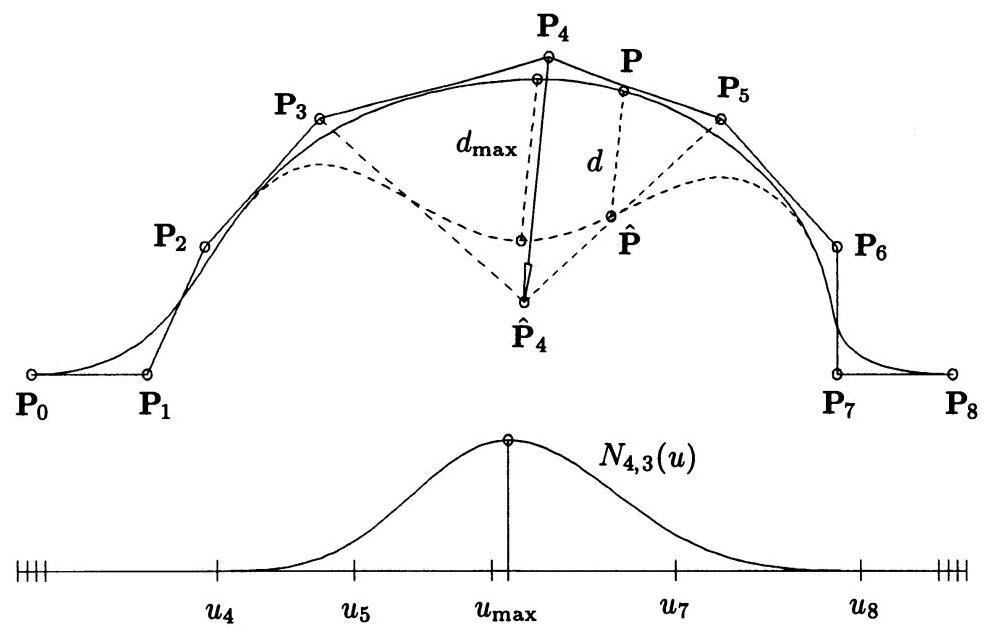
\includegraphics[max width=0.9\textwidth]{images/0193ba0d-ab19-7138-9798-cb281ce60de0_516_271_1401_990_633_0.jpg}
\end{center}
\hspace*{3em} 

图 11.1。通过重新定位 \({\mathbf{P}}_{4}\) 移动 \(\mathbf{P} = \mathbf{C}\left( {\bar{u} = 3/5}\right)\) ；相应的节点是 \({t}_{4} = {0.52}\) ，曲线的度数为三。

从用户界面的角度来看，控制点重新定位有两种广泛的方法，区别在于用户是选择控制多边形还是曲线。在第一种情况下，用户可能会指定一个向量方向和距离，然后选择控制多边形上的一个点。如果选择的点是一个现有的控制点，系统会简单地平移它并重新绘制曲线。如果不是，那么系统通过逆节点插入将该点变为控制点(见第5章，方程[5.19]-[5.21])，然后平移新的控制点并重新绘制曲线。在第二种情况下，设计师选择一个曲线点 \(\mathbf{P}\) (系统由此计算 \(\bar{u}\) )，然后选择要移动到的点 \(\widehat{\mathbf{P}}\) (系统由此计算 \(d\) 和 \(\mathbf{V}\) )。系统需要选择一个控制点 \({\mathbf{P}}_{k}\) 进行平移，以产生 \(\mathbf{P}\) 所需的移动。一般来说，最多有 \(p + 1\) 个候选者，但通常希望选择 \({\mathbf{P}}_{k}\) ，使得 \({R}_{k,p}\left( u\right)\) 成为其最大值最接近 \(\bar{u}\) 的基函数。一个通常相当接近(但不一定重合于)任意基函数最大值的参数值 \({R}_{i,p}\left( u\right)\) 被称为节点 \({t}_{i}\) ，其定义为(见[Ries73])。

\[
{t}_{i} = \frac{1}{p}\mathop{\sum }\limits_{{j = 1}}^{p}{u}_{i + j}\;i = 0,\ldots ,n \tag{11.4}
\]

注意， \({t}_{i}\) 是位于 \({R}_{i,p}\left( u\right)\) 非零域内的节点的平均值。对于交互式控制点重新定位，我们建议基于节点值选择 \(k\) ，而不是实际计算 \({R}_{i,p}\left( u\right)\) 的最大值；也就是说，选择 \(k\) 使得

\[
\left| {\bar{u} - {t}_{k}}\right|  = \mathop{\min }\limits_{i}\left| {\bar{u} - {t}_{i}}\right|  \tag{11.5}
\]

当然，这些节点可以作为起始值，通过牛顿迭代法来寻找最大值。

图 11.2 和 11.3 显示了两个控制点重新定位的情况，其中索引 \(k\) 是基于 \(\bar{u}\) 与节点的接近度选择的。注意，图 11.2 是令人愉悦的，而图 11.3 是不对称且不令人愉悦的。原因在于，在图 \({11.2}\bar{u}\) 中非常接近节点 \({t}_{k}\) (并且接近 \({R}_{k,p}\left( u\right)\) 的最大值)，因此曲线的平移在 \(\mathbf{C}\left( \bar{u}\right)\) 周围是相当对称的，并且在那里大致达到最大值。在图 11.3 中， \(\bar{u}\) 位于 \({t}_{k}\) 和 \({t}_{k + 1}\) 之间的中点(但选择了 \({t}_{k}\) )，因此最大平移发生在 \(\mathbf{C}\left( \bar{u}\right)\) 的左侧。对此困境有两种解决方案:

\begin{itemize}
\item 插入一个节点，以便将一个节点放置在 \(\bar{u}\) ；
\end{itemize}

\begin{itemize}
\item 重新定位 \({\mathbf{P}}_{k}\) 和 \({\mathbf{P}}_{k + 1}\) 。
\end{itemize}

让我们插入节点 \(\widehat{u}\) ，这迫使 \({t}_{k + 1}\) (新的 \(\left( {k + 1}\right)\) 阶节点)具有值 \(\bar{u}\) 。从方程 (11.4) 可以清楚地看出 \({u}_{k + 1} < \widehat{u} < {u}_{k + p + 1}\) ，因此

\[
\bar{u} = {t}_{k + 1} = \frac{1}{p}\left( {\widehat{u} + \mathop{\sum }\limits_{{j = 2}}^{p}{u}_{k + j}}\right)
\]

和

\[
\widehat{u} = p\bar{u} - \mathop{\sum }\limits_{{j = 2}}^{p}{u}_{k + j} \tag{11.6}
\]

\begin{center}
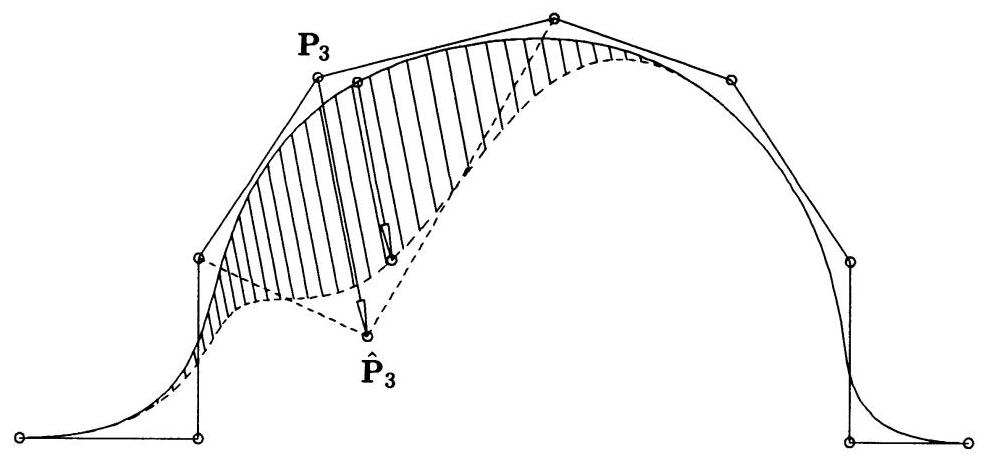
\includegraphics[max width=0.9\textwidth]{images/0193ba0d-ab19-7138-9798-cb281ce60de0_518_278_266_984_460_0.jpg}
\end{center}
\hspace*{3em} 

图 11.2。通过重新定位 \({\mathbf{P}}_{3}\) 移动 \(\mathbf{P} = \mathbf{C}\left( {\bar{u} = {0.37}}\right)\) ；相应的节点是 \({t}_{3} = {0.35}\) ，曲线的度数为三。注意曲线一段的平行平移。

图11.4显示了图11.3的曲线。将来自方程(11.6)的节点 \(\widehat{u}\) 插入，以强制 \(\bar{u}\) 成为第 \(\left( {k + 1}\right)\) 个节点。然后将得到的 \({\mathbf{Q}}_{k + 1}\) 移动以实现所需的曲线修改。请注意对称性和变化域的减小。我们提醒读者， \(\widehat{u}\) 可能已经是一个节点，插入它可能是不必要的。例如，设 \(\mathbf{C}\left( u\right)\) 为图11.5中的二次曲线。节点为 \({t}_{i} = \{ 0,1/8,3/8,5/8,7/8,1\}\) 。如果设计者选择了点，使得 \(\bar{u} = 1/2\) ，那么根据方程(11.6)有 \(\widehat{u} = 1/2\) 。如果插入 \(\widehat{u} = 1/2\) ，则 \(\bar{u}\) 成为节点 \({t}_{3}\) ，如果移动 \({\mathbf{Q}}_{3}\left( { = \mathbf{C}\left( {1/2}\right) }\right)\) ，则得到的曲线在 \(u = 1/2\) 处有一个尖点，如图11.5所示。

假设我们现在想要沿着 \(\mathbf{V}\) 移动 \(\mathbf{P} = \mathbf{C}\left( \bar{u}\right)\) 一个距离 \(d\) ，通过在 \(\mathbf{V}\) 方向上平移 \({\mathbf{P}}_{k}\) 和 \({\mathbf{P}}_{k + 1}\) (假设 \(\bar{u} \in  \left\lbrack  {{u}_{k + 1},{u}_{k + p + 1}}\right)\) )。设定

\begin{center}
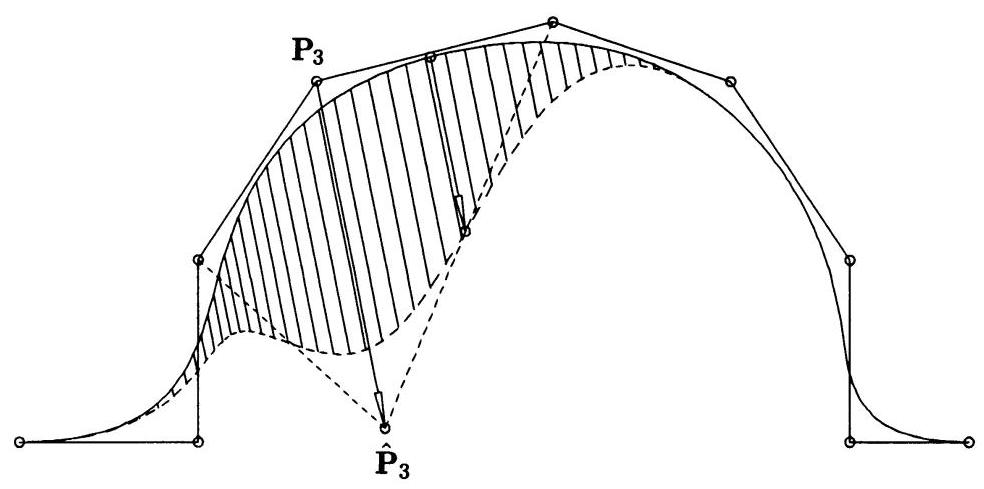
\includegraphics[max width=0.9\textwidth]{images/0193ba0d-ab19-7138-9798-cb281ce60de0_518_271_1548_984_489_0.jpg}
\end{center}
\hspace*{3em} 

图11.3。通过重新定位 \({\mathbf{P}}_{3}.\bar{u} = {0.43} = 1/2\left( {{t}_{3} + {t}_{4}}\right)\) 移动 \(\mathbf{P} = \mathbf{C}\left( \bar{u}\right)\) ；对应的节点是 \({t}_{3} = {0.35}\) ，曲线的度数为三。

\begin{center}
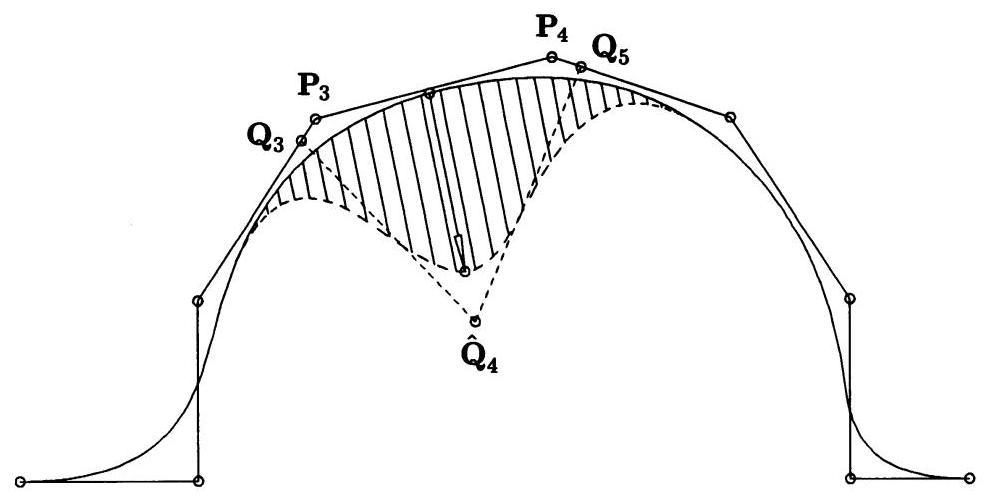
\includegraphics[max width=0.9\textwidth]{images/0193ba0d-ab19-7138-9798-cb281ce60de0_519_273_269_985_500_0.jpg}
\end{center}
\hspace*{3em} 

图11.4。通过节点插入获得的新控制点的重新定位；曲线的度数为三。

\(0 \leq  \gamma  \leq  1\) ，我们设定

\[
{\widehat{\mathbf{P}}}_{k} = {\mathbf{P}}_{k} + \left( {1 - \gamma }\right) \alpha \mathbf{V}
\]

\[
{\widehat{\mathbf{P}}}_{k + 1} = {\mathbf{P}}_{k + 1} + {\gamma \alpha }\mathbf{V} \tag{11.7}
\]

参数 \(\gamma\) 允许我们在一个线性尺度上变化 \({\mathbf{P}}_{k}\) 和 \({\mathbf{P}}_{k + 1}\) 之间的相对移动。设计者可以设定 \(\gamma\) ，或者一个好的默认值是

\[
\gamma  = \frac{\bar{u} - {t}_{k}}{{t}_{k + 1} - {t}_{k}} \tag{11.8}
\]

其中 \({t}_{k} \leq  \bar{u} \leq  {t}_{k + 1}\) 。根据平移不变性(P4.9)，我们有

\[
\left| {\widehat{\mathbf{P}} - \mathbf{P}}\right|  = d = \left| {\left( {1 - \gamma }\right) \alpha \mathbf{V}{R}_{k,p}\left( \bar{u}\right)  + {\gamma \alpha }\mathbf{V}{R}_{k + 1,p}\left( \bar{u}\right) }\right|
\]

这意味着

\[
\alpha  = \frac{d}{\left| \mathbf{V}\right| \left\lbrack  {\left( {1 - \gamma }\right) {R}_{k,p}\left( \bar{u}\right)  + \gamma {R}_{k + 1,p}\left( \bar{u}\right) }\right\rbrack  } \tag{11.9}
\]

\begin{center}
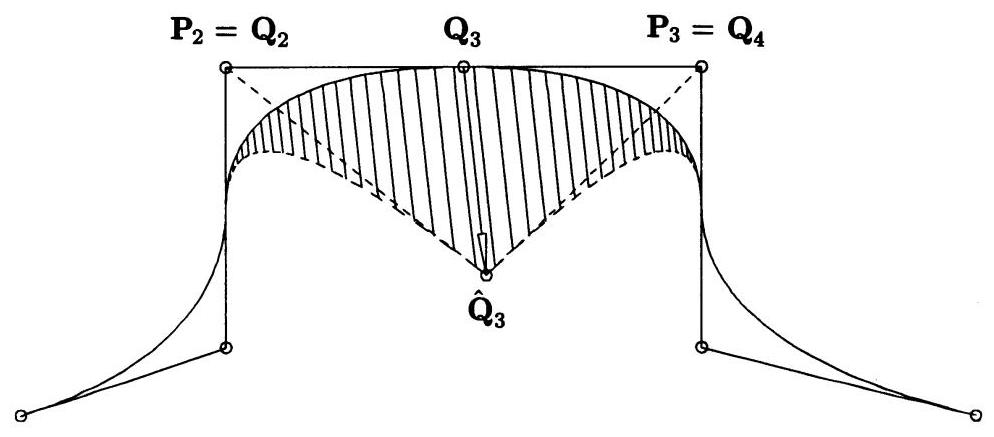
\includegraphics[max width=0.9\textwidth]{images/0193ba0d-ab19-7138-9798-cb281ce60de0_519_271_1620_994_437_0.jpg}
\end{center}
\hspace*{3em} 

图 11.5. 通过节点插入获得的新控制点的重新定位；曲线的度数为二。

图 11.6a 显示了图 11.3 的曲线。 \({\mathbf{P}}_{3}\) 和 \({\mathbf{P}}_{4}\) 都被移动了，使用了 \(\gamma  = {0.47}\) (由公式 [11.8] 计算的默认值)。显然，这种方法的缺点是变化的范围更广，即 \(\left\lbrack  {{u}_{k},{u}_{k + p + 2}}\right)\) 。在图 11.6b 中， \({\mathbf{P}}_{3}\) 和 \({\mathbf{P}}_{4}\) 被移动，使用了 \(\gamma  = 4/5\) 。

使用这些工具，可以轻松实现一个用户友好、互动式的图形界面，用于控制点的重新定位。注意，当 \({\mathbf{P}}_{k}\) 沿相同的向量方向反复平移时，公式 (11.3) 中的值 \({R}_{k,p}\left( \bar{u}\right)\) 不会改变(因此 \(\alpha\) 也不会改变)。此外，只有曲线中 \(\left\lbrack  {{u}_{k},{u}_{k + p + 1}}\right)\) 的图像部分需要在每次重新定位时进行图形更新。图 11.7 显示了一个控制点的增量重新定位。指定了一个增量 \({\Delta d}\) ，它固定了一个 \({\Delta \alpha }\) 。相关的控制点然后被平移一个增量 \({\Delta \alpha }\mathbf{V}\) ，并且在每次激活指定的图形输入时，相关的曲线段被重新绘制。

\begin{center}
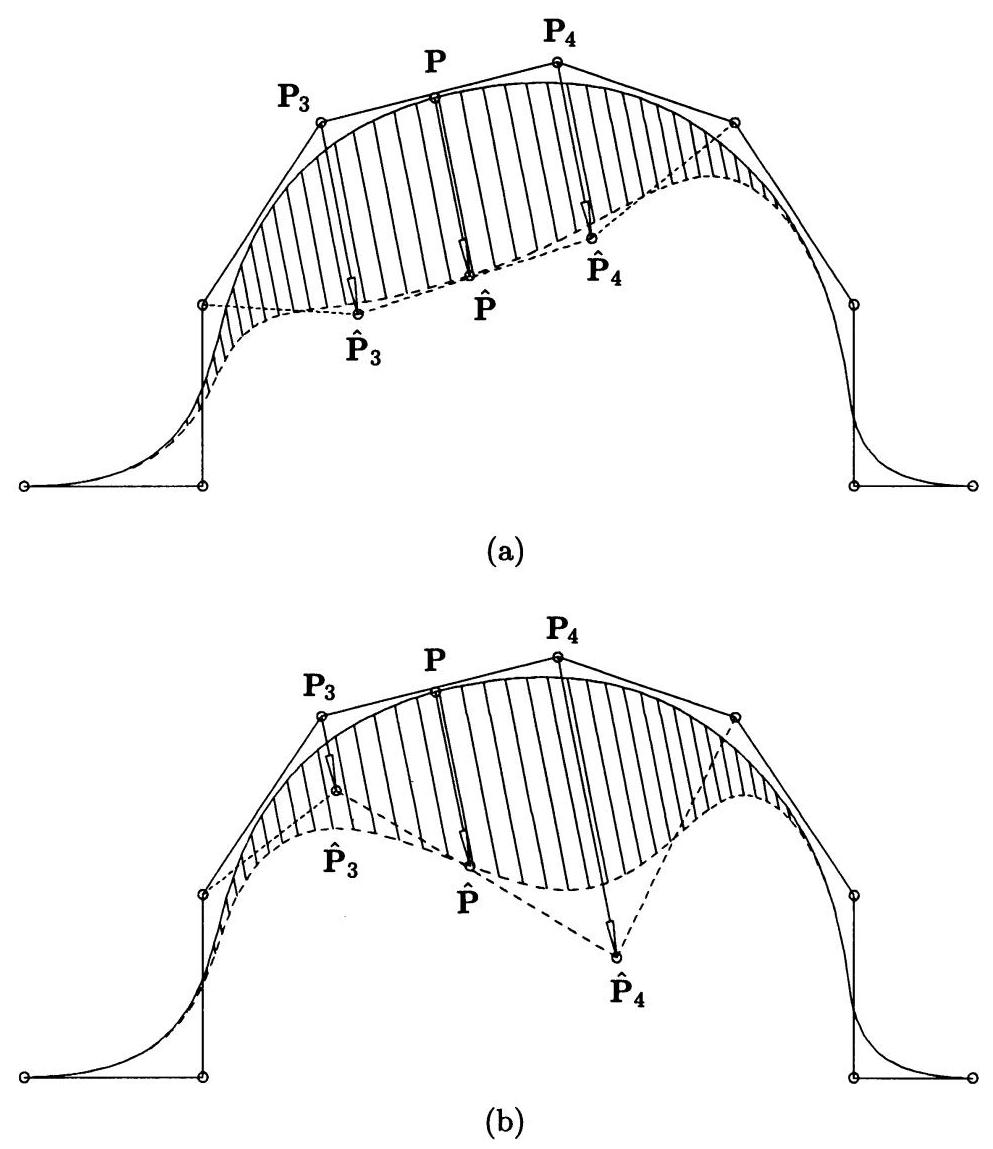
\includegraphics[max width=0.9\textwidth]{images/0193ba0d-ab19-7138-9798-cb281ce60de0_520_269_916_993_1149_0.jpg}
\end{center}
\hspace*{3em} 

图 11.6. 同时重新定位 \({\mathbf{P}}_{3}\) 和 \({\mathbf{P}}_{4};\bar{u} = {0.43}\) 。 (a) \(\gamma  = {0.47}\) (默认)；(b) \(\gamma  = 4/5\) 。

最后，设计师可以通过选择两个额外的曲线点 \({\mathbf{Q}}_{1}\) 和 \({\mathbf{Q}}_{2}\) 来轻松限制曲线应变化的域，这两个点确定参数 \({\bar{u}}_{1}\) 和 \({\bar{u}}_{2}\) ，满足 \({\bar{u}}_{1} < \bar{u} < {\bar{u}}_{2}\) 。如果 \({\bar{u}}_{1}\) 和 \({\bar{u}}_{2}\) 还不是节点，则每个节点插入一次。然后，如果必要的话，在区间 \(\left\lbrack  {{\bar{u}}_{1},\bar{u}}\right)\) 和 \(\left\lbrack  {\bar{u},{\bar{u}}_{2}}\right)\) 上插入额外的节点，以确保存在一个合适的控制点 \({\mathbf{P}}_{k}\) ，使得 \(\bar{u}\) 接近节点 \({t}_{k}\) 、 \({\bar{u}}_{1} \leq  {u}_{k}\) 和 \({u}_{k + p + 1} \leq  {\bar{u}}_{2}\) 。节点不应以大于一个的重数插入，因为这可能导致在移动控制点时出现不必要的不连续性。

这些技术可以轻松扩展到曲面。为完整性起见，我们陈述相关公式。设

\[
\mathbf{S}\left( {u,v}\right)  = \mathop{\sum }\limits_{{i = 0}}^{n}\mathop{\sum }\limits_{{j = 0}}^{m}{R}_{i,p;j,q}\left( {u,v}\right) {\mathbf{P}}_{i,j}
\]

为 NURBS 曲面，并假设 \(\mathbf{P} = \mathbf{S}\left( {\bar{u},\bar{v}}\right)\) 沿向量 \(\mathbf{V}\) 移动，距离 \(d\) ，通过重新定位控制点 \({\mathbf{P}}_{k,\ell }\) 。那么

\[
{\widehat{\mathbf{P}}}_{k,\ell } = {\mathbf{P}}_{k,\ell } + \alpha \mathbf{V} \tag{11.10}
\]

与

\[
\alpha  = \frac{d}{\left| \mathbf{V}\right| {R}_{k,\ell }\left( {\bar{u},\bar{v}}\right) } \tag{11.11}
\]

要么设计师选择 \(k\) 和 \(\ell\) ，要么系统根据 \(\bar{u}\) 和 \(\bar{v}\) 与 \(u\) 和 \(v\) 节点 \({s}_{i}\) 和 \({t}_{j}\) 的接近程度来选择它们，这些节点由

\[
{s}_{i} = \frac{1}{p}\mathop{\sum }\limits_{{r = 1}}^{p}{u}_{i + r}\;i = 0,\ldots ,n
\]

\[
{t}_{j} = \frac{1}{q}\mathop{\sum }\limits_{{r = 1}}^{q}{v}_{j + r}\;j = 0,\ldots ,m \tag{11.12}
\]

使用类似于公式 (11.6) 的公式，可以计算并插入一个 \(u\) 或 \(v\) 节点，或两者，以减少变化的域，并将 \(\bar{u}\) 和/或 \(\bar{v}\) 移动到节点位置。如果 \(0 \leq  \delta ,\gamma  \leq  1\) ，那么 \({\mathbf{P}}_{k,\ell },{\mathbf{P}}_{k + 1,\ell },{\mathbf{P}}_{k,\ell  + 1}\) 和 \({\mathbf{P}}_{k + 1,\ell  + 1}\) 可以同时沿着 \(\mathbf{V}\) 的方向移动。

\[
{\widehat{\mathbf{P}}}_{k,\ell } = {\mathbf{P}}_{k,\ell } + \left( {1 - \delta }\right) \left( {1 - \gamma }\right) \alpha \mathbf{V}
\]

\[
{\widehat{\mathbf{P}}}_{k + 1,\ell } = {\mathbf{P}}_{k + 1,\ell } + \delta \left( {1 - \gamma }\right) \alpha \mathbf{V}
\]

\[
{\widehat{\mathbf{P}}}_{k,\ell  + 1} = {\mathbf{P}}_{k,\ell  + 1} + \left( {1 - \delta }\right) {\gamma \alpha }\mathbf{V}
\]

\[
{\widehat{\mathbf{P}}}_{k + 1,\ell  + 1} = {\mathbf{P}}_{k + 1,\ell  + 1} + {\delta \gamma \alpha }\mathbf{V} \tag{11.13}
\]

(11.14)

\begin{center}
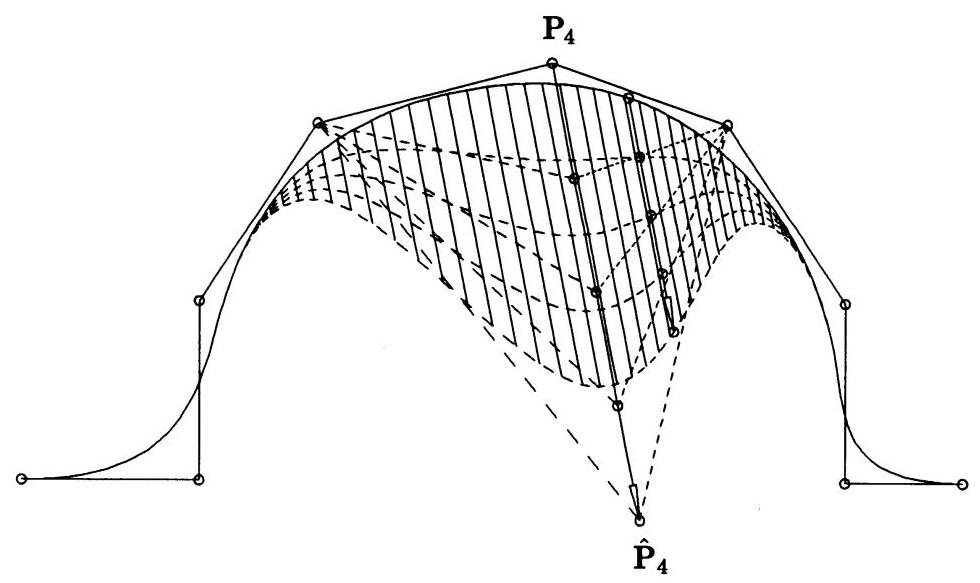
\includegraphics[max width=0.9\textwidth]{images/0193ba0d-ab19-7138-9798-cb281ce60de0_522_278_250_980_583_0.jpg}
\end{center}
\hspace*{3em} 

图 11.7。通过重新定位 \({\mathbf{P}}_{4};\bar{u} = 3/5\) 以相等的增量拉动曲线。

\begin{center}
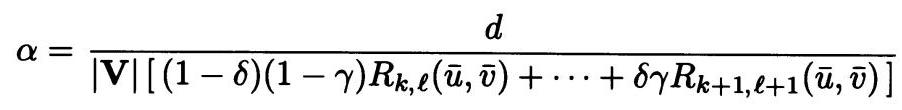
\includegraphics[max width=0.8\textwidth]{images/0193ba0d-ab19-7138-9798-cb281ce60de0_522_301_976_902_110_0.jpg}
\end{center}
\hspace*{3em} 

图 11.8a 和 11.8b 显示了一个控制点的转换，图 11.9a 和 11.9b 则说明了四个相邻控制点的同时移动。

\begin{center}
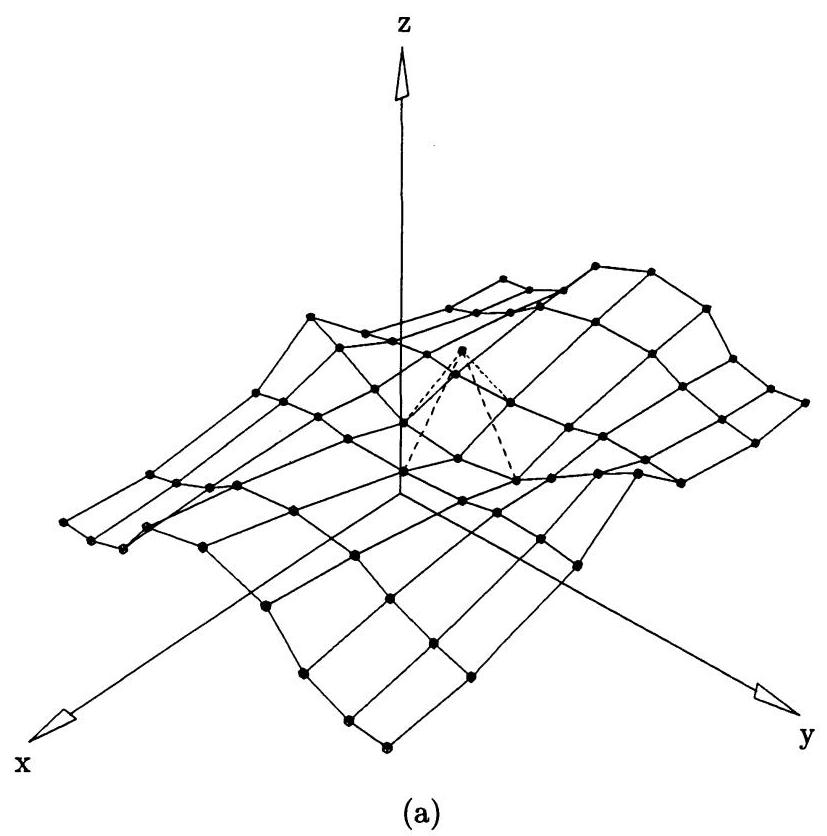
\includegraphics[max width=0.7\textwidth]{images/0193ba0d-ab19-7138-9798-cb281ce60de0_522_348_1252_827_836_0.jpg}
\end{center}
\hspace*{3em} 

图 11.8. 重新定位 \({\mathbf{P}}_{4,3}\) ，与 \(\bar{u} = \bar{v} = {0.55}\) 。 (a) 控制网；(b) 一个表面，其局部补丁沿控制点移动的方向平行移动。

\begin{center}
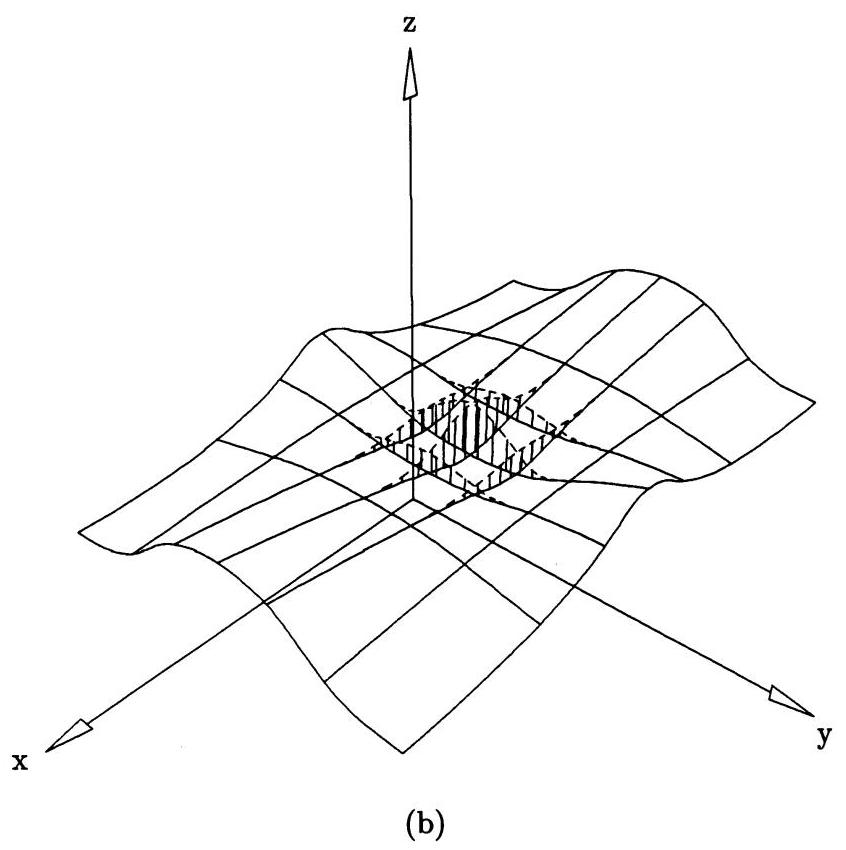
\includegraphics[max width=0.7\textwidth]{images/0193ba0d-ab19-7138-9798-cb281ce60de0_523_348_238_846_850_0.jpg}
\end{center}
\hspace*{3em} 

图 11.8. (续)。

类似于曲线情况，节点插入可以用来限制表面变化的矩形域，而逆节点插入可以用来在表面控制网的边缘指定位置获取额外的控制点。点 \({\mathbf{Q}}_{u}\) 在 \(u\) 方向上，由公式插入。

\[
\widehat{u} = {u}_{k + 1} + \alpha \left( {{u}_{k + p + 1} - {u}_{k + 1}}\right)  \tag{11.15}
\]

与

\[
\alpha  = \frac{{w}_{k,\ell }\left| {{\mathbf{Q}}_{u} - {\mathbf{P}}_{k,\ell }}\right| }{{w}_{k,\ell }\left| {{\mathbf{Q}}_{u} - {\mathbf{P}}_{k,\ell }}\right|  + {w}_{k + 1,\ell }\left| {{\mathbf{P}}_{k + 1,\ell } - {\mathbf{Q}}_{u}}\right| }
\]

(见 [Pieg89d])。同样， \({\mathbf{Q}}_{v}\) 由以下公式插入。

\[
\widehat{v} = {v}_{\ell  + 1} + \beta \left( {{v}_{\ell  + q + 1} - {v}_{\ell  + 1}}\right)  \tag{11.16}
\]

与

\[
\beta  = \frac{{w}_{k,\ell }\left| {{\mathbf{Q}}_{v} - {\mathbf{P}}_{k,\ell }}\right| }{{w}_{k,\ell }\left| {{\mathbf{Q}}_{v} - {\mathbf{P}}_{k,\ell }}\right|  + {w}_{k,\ell  + 1}\left| {{\mathbf{P}}_{k,\ell  + 1} - {\mathbf{Q}}_{v}}\right| }
\]



\section{权重修改}

在本节中，我们研究修改权重的效果，特别是对曲线的一个或两个相邻权重，以及对表面的一个权重。

\begin{center}
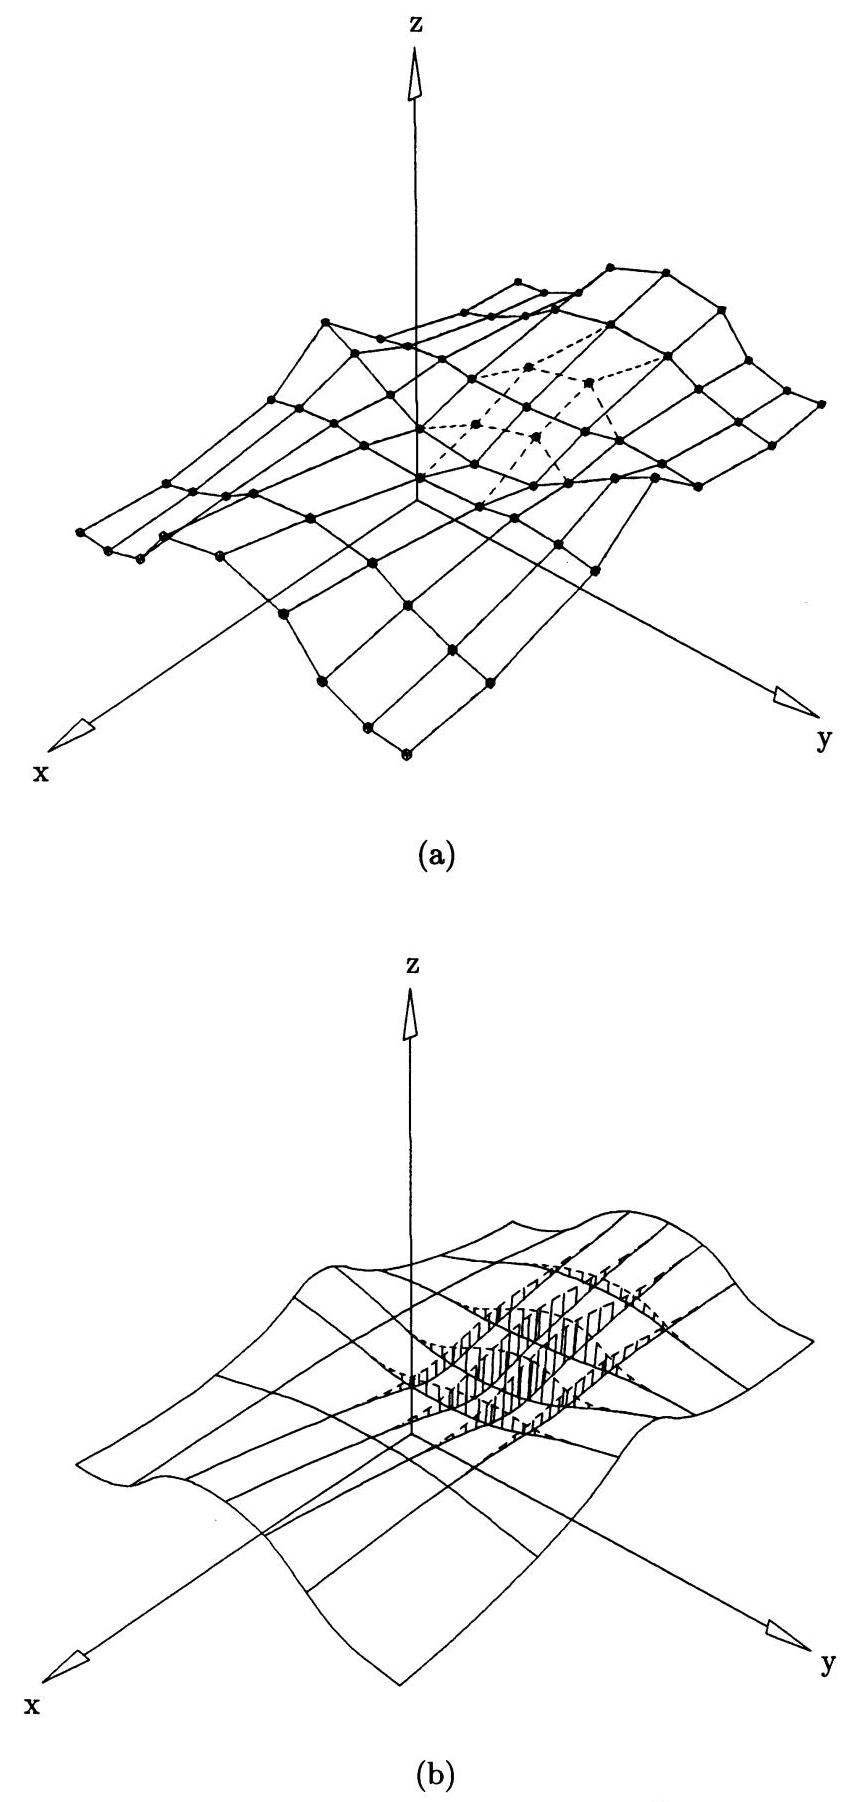
\includegraphics[max width=0.7\textwidth]{images/0193ba0d-ab19-7138-9798-cb281ce60de0_524_339_241_867_1802_0.jpg}
\end{center}
\hspace*{3em} 

图 11.9. 重新定位四个表面控制点 \({\mathbf{P}}_{4,3},{\mathbf{P}}_{5,3},{\mathbf{P}}_{4,4}\) 和 \({\mathbf{P}}_{5,4}\) ，与 \(\bar{u} = \bar{v} = 3/5\) 。 (a) 控制网；(b) 一个表面，其局部补丁沿控制点移动的方向平行移动。



\subsection{单曲线权重的修改}
让

\[
\mathbf{C}\left( u\right)  = \mathop{\sum }\limits_{{i = 0}}^{n}{R}_{i,p}\left( u\right) {\mathbf{P}}_{i} \tag{11.17}
\]

设为 NURBS 曲线，且 \(\bar{u}\) 为满足 \(\bar{u} \in  \left\lbrack  {{u}_{k},{u}_{k + p + 1}}\right)\) 的固定参数值。我们在第 4 章中指出，修改权重 \({w}_{k}\) 的值的效果是将点 \(\mathbf{C}\left( \bar{u}\right)\) 沿着由 \({\mathbf{P}}_{k}\) 和原始点 \(\mathbf{C}\left( \bar{u}\right)\) 定义的直线移动(见图 4.2、4.4 和 4.6)。因此，虽然控制点的重新定位对曲线有平移效果，但权重的修改具有透视效果，其中受影响域内的所有曲线点沿着与对应于被修改权重的控制点相交的直线被拉动(或推送)。在本节中，我们证明这一陈述，并建立权重的精确几何意义。

权重 \({w}_{k}\) 可以被视为方程 (11.17) 中的一个变量，因此我们可以对 \(\mathbf{C}\left( u\right)\) 关于 \({w}_{k}\) 进行微分。使用恒等式

\[
{R}_{k,p}\left( u\right)  = \frac{{N}_{k,p}\left( u\right) {w}_{k}}{\mathop{\sum }\limits_{{r = 0}}^{n}{N}_{r,p}\left( u\right) {w}_{r}}
\]

以及微分的商法则，我们得到

\[
\frac{\partial }{\partial {w}_{k}}\mathbf{C}\left( {u;{w}_{0},\ldots ,{w}_{n}}\right)  = \frac{\partial }{\partial {w}_{k}}\mathop{\sum }\limits_{{i = 0}}^{n}{R}_{i,p}\left( u\right) {\mathbf{P}}_{i}
\]

\[
= \mathop{\sum }\limits_{{i \neq  k}}\frac{-{N}_{i,p}\left( u\right) {w}_{i}{N}_{k,p}\left( u\right) }{{\left( \mathop{\sum }\limits_{{r = 0}}^{n}{N}_{r,p}\left( u\right) {w}_{r}\right) }^{2}}{\mathbf{P}}_{i}
\]

\[
+ \frac{{N}_{k,p}\left( u\right) \left( {\mathop{\sum }\limits_{{r = 0}}^{n}{N}_{r,p}\left( u\right) {w}_{r}}\right)  - {N}_{k,p}\left( u\right) {N}_{k,p}\left( u\right) {w}_{k}}{{\left( \mathop{\sum }\limits_{{r = 0}}^{n}{N}_{r,p}\left( u\right) {w}_{r}\right) }^{2}}{\mathbf{P}}_{k}
\]

\[
= \mathop{\sum }\limits_{{i \neq  k}}\frac{-{N}_{k,p}\left( u\right) }{\mathop{\sum }\limits_{{r = 0}}^{n}{N}_{r,p}\left( u\right) {w}_{r}}{R}_{i,p}\left( u\right) {\mathbf{P}}_{i}
\]

\[
+ \frac{{R}_{k,p}}{{w}_{k}}{\mathbf{P}}_{k} - \frac{{N}_{k,p}\left( u\right) {R}_{k,p}\left( u\right) }{\mathop{\sum }\limits_{{r = 0}}^{n}{N}_{r,p}\left( u\right) {w}_{r}}{\mathbf{P}}_{k}
\]

\[
= \frac{{R}_{k,p}\left( u\right) }{{w}_{k}}\left( {{\mathbf{P}}_{k} - \mathop{\sum }\limits_{{r = 0}}^{n}{R}_{r,p}\left( u\right) {\mathbf{P}}_{r}}\right)
\]

\[
= \frac{{R}_{k,p}\left( u\right) }{{w}_{k}}\left( {{\mathbf{P}}_{k} - \mathbf{C}\left( u\right) }\right)  = \alpha \left( {k,u}\right) \left( {{\mathbf{P}}_{k} - \mathbf{C}\left( u\right) }\right)  \tag{11.18}
\]

因此，关于 \({w}_{k}\) 的 \(\mathbf{C}\left( u\right)\) 的一阶导数是一个指向从 \(\mathbf{C}\left( u\right)\) 到 \({\mathbf{P}}_{k}\) 方向的向量。我们现在通过归纳法证明所有阶的导数具有这种形式。设 \({\alpha }^{\left( 1\right) } = \alpha \left( {k,u}\right)\) ，并假设 \(n\) 阶导数具有形式 \({\alpha }^{\left( n\right) }\left( {{\mathbf{P}}_{k} - \mathbf{C}\left( u\right) }\right)\) 。那么

\[
\frac{{\partial }^{n + 1}\mathbf{C}\left( u\right) }{\partial {w}_{k}^{n + 1}} = \frac{\partial \left\lbrack  {{\alpha }^{\left( n\right) }\left( {{\mathbf{P}}_{k} - \mathbf{C}\left( u\right) }\right) }\right\rbrack  }{\partial {w}_{k}}
\]

\[
= {\alpha }^{\left( n\right) }\left( {-{\alpha }^{\left( 1\right) }{\mathbf{P}}_{k} + {\alpha }^{\left( 1\right) }\mathbf{C}\left( u\right) }\right)  + \frac{\partial {\alpha }^{\left( n\right) }}{\partial {w}_{k}}\left( {{\mathbf{P}}_{k} - \mathbf{C}\left( u\right) }\right)
\]

\[
= \left( {\frac{\partial {\alpha }^{\left( n\right) }}{\partial {w}_{k}} - {\alpha }^{\left( 1\right) }{\alpha }^{\left( n\right) }}\right) \left( {{\mathbf{P}}_{k} - \mathbf{C}\left( u\right) }\right)  = {\alpha }^{\left( n + 1\right) }\left( {{\mathbf{P}}_{k} - \mathbf{C}\left( u\right) }\right)
\]

其中

\[
{\alpha }^{\left( n + 1\right) } = \frac{\partial {\alpha }^{\left( n\right) }}{\partial {w}_{k}} - {\alpha }^{\left( 1\right) }{\alpha }^{\left( n\right) }
\]

这完成了证明。

容易推导出一个递归公式来计算 \({\alpha }^{\left( n + 1\right) }\) ，从而获得高阶导数的公式

\[
\frac{{\partial }^{n + 1}\mathbf{C}\left( u\right) }{\partial {w}_{k}^{n + 1}} = {\alpha }^{\left( n + 1\right) }\left( {{\mathbf{P}}_{k} - \mathbf{C}\left( u\right) }\right) \;n = 1,2,\ldots ,\infty  \tag{11.19}
\]

具有

\[
{\alpha }^{\left( n + 1\right) } = \left( {-1}\right) \left( {n + 1}\right) {\alpha }^{\left( n\right) }{\alpha }^{\left( 1\right) } \tag{11.20}
\]

方程 (11.18)-(11.20) 证明了任意曲线点 \(\mathbf{C}\left( u\right)\) 随着 \({w}_{k}\) 值的增加而沿直线朝向 \({\mathbf{P}}_{k}\) 移动。

现在我们采取一种更几何的方法。从方程 (11.17) 的曲线开始，让 \({w}_{k}\) 变化， \(0 \leq  {w}_{k} < \infty\) 。将结果曲线的家族记为 \(\mathbf{C}\left( {u;{w}_{k}}\right)\) (见图 11.10)。假设 \(\bar{u} \in  \left\lbrack  {{u}_{k},{u}_{k + p + 1}}\right)\) ，并定义点

\[
\mathbf{R} = \mathbf{C}\left( {\bar{u};{w}_{k} = 0}\right)
\]

\[
\mathbf{M} = \mathbf{C}\left( {\bar{u};{w}_{k} = 1}\right)
\]

\[
\mathbf{P} = \mathbf{C}\left( {\bar{u};{w}_{k} \neq  0,1}\right)  \tag{11.21}
\]

注意到 \(\mathbf{R}\) 和 \(\mathbf{M}\) 是特定曲线上的点，但 \(\mathbf{P}\) 可以位于 \(\mathbf{R}\) 和 \({\mathbf{P}}_{k}\) 之间的任何位置，因为 \({w}_{k} \geq  0\) 。现在 \(\mathbf{M}\) 和 \(\mathbf{P}\) 可以表示为

\[
\mathbf{M} = \left( {1 - s}\right) \mathbf{R} + s{\mathbf{P}}_{k}
\]

\[
\mathbf{P} = \left( {1 - t}\right) \mathbf{R} + t{\mathbf{P}}_{k} \tag{11.22}
\]

\begin{center}
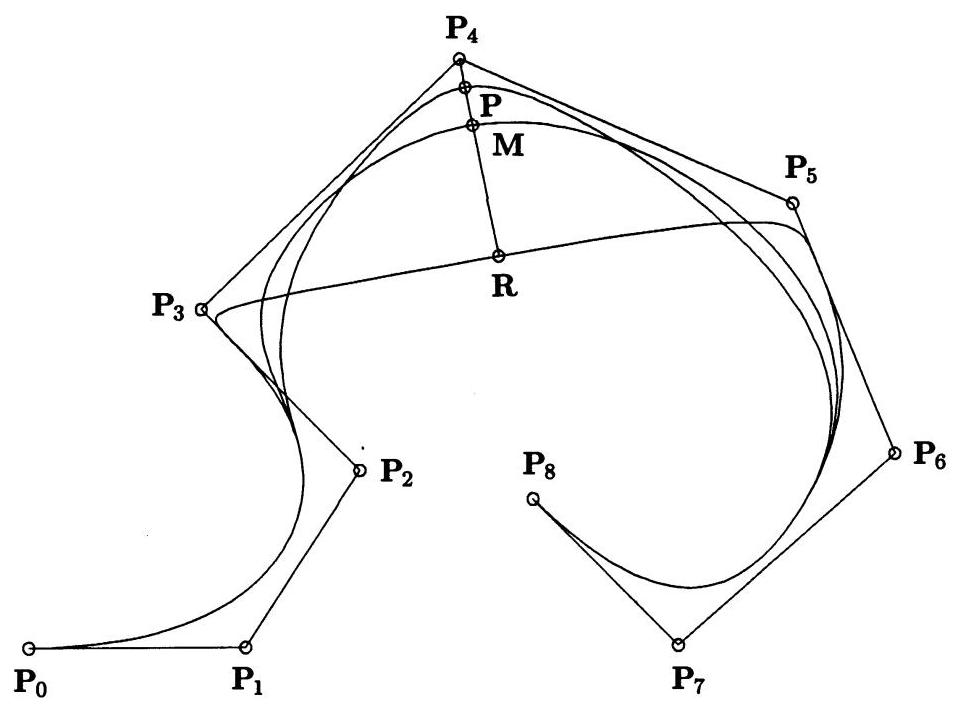
\includegraphics[max width=0.8\textwidth]{images/0193ba0d-ab19-7138-9798-cb281ce60de0_527_291_254_956_710_0.jpg}
\end{center}
\hspace*{3em} 

图 11.10. 权重的几何意义。

其中

\[
s = \frac{{N}_{k,p}\left( \bar{u}\right) }{\mathop{\sum }\limits_{{i \neq  k}}{N}_{i,p}\left( \bar{u}\right) {w}_{i} + {N}_{k,p}\left( \bar{u}\right) }
\]

\[
t = \frac{{N}_{k,p}\left( \bar{u}\right) {w}_{k}}{\mathop{\sum }\limits_{{i = 0}}^{n}{N}_{i,p}\left( \bar{u}\right) {w}_{i}} = {R}_{k,p}\left( \bar{u}\right)  \tag{11.23}
\]

为了推导这些方程，注意到

\[
\mathbf{R} = \frac{\mathop{\sum }\limits_{{i \neq  k}}{N}_{i,p}\left( \bar{u}\right) {w}_{i}{\mathbf{P}}_{i}}{\mathop{\sum }\limits_{{i \neq  k}}{N}_{i,p}\left( \bar{u}\right) {w}_{i}}\;{w}_{k} = 0
\]

因此我们有

\[
\mathbf{P} = \mathop{\sum }\limits_{{i = 0}}^{n}{R}_{i,p}\left( \bar{u}\right) {\mathbf{P}}_{i} = \mathop{\sum }\limits_{{i \neq  k}}{R}_{i,p}\left( \bar{u}\right) {\mathbf{P}}_{i} + {R}_{k,p}\left( \bar{u}\right) {\mathbf{P}}_{k}
\]

\[
= \frac{\mathop{\sum }\limits_{{i \neq  k}}{N}_{i,p}\left( \bar{u}\right) {w}_{i}{\mathbf{P}}_{i}}{\mathop{\sum }\limits_{{i = 0}}^{n}{N}_{i,p}\left( \bar{u}\right) {w}_{i}} + {R}_{k,p}\left( \bar{u}\right) {\mathbf{P}}_{k}
\]

\[
= \frac{\mathop{\sum }\limits_{{i \neq  k}}{N}_{i,p}\left( \bar{u}\right) {w}_{i}}{\mathop{\sum }\limits_{{i = 0}}^{n}{N}_{i,p}\left( \bar{u}\right) {w}_{i}}\mathbf{R} + {R}_{k,p}\left( \bar{u}\right) {\mathbf{P}}_{k}
\]

\[
= \left( {\frac{\mathop{\sum }\limits_{{i = 0}}^{n}{N}_{i,p}\left( \bar{u}\right) {w}_{i}}{\mathop{\sum }\limits_{{i = 0}}^{n}{N}_{i,p}\left( \bar{u}\right) {w}_{i}} - \frac{{N}_{k,p}\left( \bar{u}\right) {w}_{k}}{\mathop{\sum }\limits_{{i = 0}}^{n}{N}_{i,p}\left( \bar{u}\right) {w}_{i}}}\right) \mathbf{R} + {R}_{k,p}\left( \bar{u}\right) {\mathbf{P}}_{k}
\]

\[
= \left( {1 - {R}_{k,p}\left( \bar{u}\right) }\right) \mathbf{R} + {R}_{k,p}\left( \bar{u}\right) {\mathbf{P}}_{k} = \left( {1 - t}\right) \mathbf{R} + t{\mathbf{P}}_{k}
\]

其中 \(t = {R}_{k,p}\left( \bar{u}\right)\) 。最后，设定 \({w}_{k} = 1\) 得到

\[
\mathbf{M} = \frac{\mathop{\sum }\limits_{{i \neq  k}}{N}_{i,p}\left( \bar{u}\right) {w}_{i}{\mathbf{P}}_{i}}{\mathop{\sum }\limits_{{i \neq  k}}{N}_{i,p}\left( \bar{u}\right) {w}_{i} + {N}_{k,p}\left( \bar{u}\right) } + \frac{{N}_{k,p}\left( \bar{u}\right) }{\mathop{\sum }\limits_{{i \neq  k}}{N}_{i,p}\left( \bar{u}\right) {w}_{i} + {N}_{k,p}\left( \bar{u}\right) }{\mathbf{P}}_{k}
\]

\[
= \frac{\mathop{\sum }\limits_{{i \neq  k}}{N}_{i,p}\left( \bar{u}\right) {w}_{i}}{\mathop{\sum }\limits_{{i \neq  k}}{N}_{i,p}\left( \bar{u}\right) {w}_{i} + {N}_{k,p}\left( \bar{u}\right) }\mathbf{R} + \frac{{N}_{k,p}\left( \bar{u}\right) }{\mathop{\sum }\limits_{{i \neq  k}}{N}_{i,p}\left( \bar{u}\right) {w}_{i} + {N}_{k,p}\left( \bar{u}\right) }{\mathbf{P}}_{k}
\]

\[
= \frac{\mathop{\sum }\limits_{{i \neq  k}}{N}_{i,p}\left( \bar{u}\right) {w}_{i} + {N}_{k,p}\left( \bar{u}\right)  - {N}_{k,p}\left( \bar{u}\right) }{\mathop{\sum }\limits_{{i \neq  k}}{N}_{i,p}\left( \bar{u}\right) {w}_{i} + {N}_{k,p}\left( \bar{u}\right) }\mathbf{R} + \frac{{N}_{k,p}\left( \bar{u}\right) }{\mathop{\sum }\limits_{{i \neq  k}}{N}_{i,p}\left( \bar{u}\right) {w}_{i} + {N}_{k,p}\left( \bar{u}\right) }{\mathbf{P}}_{k}
\]

\[
= \left( {1 - s}\right) \mathbf{R} + s{\mathbf{P}}_{k}
\]

其中

\[
s = \frac{{N}_{k,p}\left( \bar{u}\right) }{\mathop{\sum }\limits_{{i \neq  k}}{N}_{i,p}\left( \bar{u}\right) {w}_{i} + {N}_{k,p}\left( \bar{u}\right) }
\]

从方程 (11.22) 和 (11.23) 我们得到

\[
{w}_{k} = \frac{\mathop{\sum }\limits_{{i \neq  k}}{N}_{i,p}\left( \bar{u}\right) {w}_{i}}{{N}_{k,p}\left( \bar{u}\right) }/\frac{\mathop{\sum }\limits_{{i \neq  k}}{N}_{i,p}\left( \bar{u}\right) {w}_{i}}{{N}_{k,p}\left( \bar{u}\right) {w}_{k}}
\]

\[
= \frac{1 - s}{\mathrm{\;s}}/\frac{1 - t}{t} = \frac{{\mathbf{P}}_{k}\mathbf{M}}{\mathbf{{RM}}}/\frac{{\mathbf{P}}_{k}\mathbf{P}}{\mathbf{{RP}}} \tag{11.24}
\]

方程 (11.24) 表示 \({w}_{k}\) 是四个点 \({\mathbf{P}}_{k},\mathbf{R},\mathbf{M}\) 和 \(\mathbf{P}\) 的交比，记作 \(\left( {{\mathbf{P}}_{k},\mathbf{R};\mathbf{M},\mathbf{P}}\right)\) (见 [Coxe74; Boeh94])。交比是射影几何中的一个基本量。关于 NURBS 曲线的形状修改，我们提到方程 (11.21)-(11.24) 的以下结果:

\begin{itemize}
\item 当 \({w}_{k}\) 增加(减少)时， \(t\) 增加(减少)，因此曲线被拉向(推离) \({\mathbf{P}}_{k}\) 。
\end{itemize}

\begin{itemize}
\item \(\mathbf{P}\) 沿着通过 \({\mathbf{P}}_{k}\) 的直线段移动；因此，修改 \({w}_{k}\) 会以可预测的方式改变曲线；
\end{itemize}

\begin{itemize}
\item 当 \(\mathbf{P}\) 接近 \({\mathbf{P}}_{k},t\) 时， \({w}_{k}\) 趋近于无穷大。
\end{itemize}

现在假设点 \(\mathbf{P} = \mathbf{C}\left( \bar{u}\right)\) 要被拉(推)向(远离) \({\mathbf{P}}_{k}\) 到一个新的位置 \(\widehat{\mathbf{P}}\) ，通过修改 \({w}_{k}\) 。设定 \(d = \mathbf{P}\widehat{\mathbf{P}} = \left| {\mathbf{P} - \widehat{\mathbf{P}}}\right|\) 。所需的新权重 \({\widehat{w}}_{k}\) 的推导如下:

\[
{\widehat{w}}_{k} = \frac{{\mathbf{P}}_{k}\mathbf{M} \cdot  \left( {\mathbf{{RP}} \pm  d}\right) }{\mathbf{{RM}} \cdot  \left( {{\mathbf{P}}_{k}\mathbf{P} \mp  d}\right) }
\]

\[
= \frac{{\mathbf{P}}_{k}\mathbf{M} \cdot  \mathbf{{RP}}}{\mathbf{{RM}} \cdot  {\mathbf{P}}_{k}\mathbf{P} \mp  d \cdot  \mathbf{{RM}}} \pm  \frac{d \cdot  {\mathbf{P}}_{k}\mathbf{M}}{\mathbf{{RM}} \cdot  \left( {{\mathbf{P}}_{k}\mathbf{P} \mp  d}\right) }
\]

使用

\[
{w}_{k} = \frac{{\mathbf{P}}_{k}\mathbf{M} \cdot  \mathbf{{RP}}}{\mathbf{{RM}} \cdot  {\mathbf{P}}_{k}\mathbf{P}}
\]

我们得到

\[
{\widehat{w}}_{k} = \frac{{w}_{k} \cdot  {\mathbf{P}}_{k}\mathbf{P}}{{\mathbf{P}}_{k}\mathbf{P} \mp  d} \pm  \frac{d \cdot  {\mathbf{P}}_{k}\mathbf{M}}{\mathbf{{RM}} \cdot  \left( {{\mathbf{P}}_{k}\mathbf{P} \mp  d}\right) }
\]

\[
= {w}_{k}\left( {\frac{{\mathbf{P}}_{k}\mathbf{P}}{{\mathbf{P}}_{k}\mathbf{P} \mp  d} \pm  \frac{d \cdot  {\mathbf{P}}_{k}\mathbf{P}}{\mathbf{{RP}} \cdot  \left( {{\mathbf{P}}_{k}\mathbf{P} \mp  d}\right) }}\right)
\]

\[
= {w}_{k}\left( \frac{{\mathbf{P}}_{k}\mathbf{P} \cdot  \left( {\mathbf{{RP}} \pm  d}\right) }{\mathbf{{RP}} \cdot  \left( {{\mathbf{P}}_{k}\mathbf{P} \mp  d}\right) }\right)  = {w}_{k}\left( \frac{\left( {1 - t}\right) \left( {\mathbf{{RP}} \pm  d}\right) }{t \cdot  \left( {{\mathbf{P}}_{k}\mathbf{P} \mp  d}\right) }\right)
\]

\[
= {w}_{k}\left( {\frac{\left( {1 - t}\right)  \cdot  \mathbf{{RP}} \mp  {td}}{t \cdot  {\mathbf{P}}_{k}\mathbf{P} \mp  {td}} \pm  \frac{d}{t \cdot  \left( {{\mathbf{P}}_{k}\mathbf{P} \mp  d}\right) }}\right)
\]

并且从方程 (11.24) 中我们得到

\[
{\widehat{w}}_{k} = {w}_{k}\left( {1 \pm  \frac{d}{{R}_{k,p}\left( \bar{u}\right) \left( {{\mathbf{P}}_{k}\mathbf{P} \mp  d}\right) }}\right)  \tag{11.25}
\]

当 \(\pm\) 或 \(\mp\) 出现时，拉操作时取上符号，推操作时取下符号 [Pieg89c]。

为了实现一个用户界面以修改一个曲线权重，设计者在曲线上选择一个点 \(\mathbf{P}\) 和控制多边形上的一个点。系统计算参数 \(\bar{u}\) 使得 \(\mathbf{P} = \mathbf{C}\left( \bar{u}\right)\) 。如果在控制多边形上选择的点还不是控制点，系统通过使用逆节点插入将其变为控制点。将控制点表示为 \({\mathbf{P}}_{k}\) 。然后系统通过 \(\mathbf{P}\) 和 \({\mathbf{P}}_{k}\) 画一条线。设计者在这条线上选择点 \(\widehat{\mathbf{P}}\) ，允许系统计算 \(d\) ，最后从方程 (11.25) 中得到 \({\widehat{w}}_{k}\) 。读者应注意到

\begin{itemize}
\item 两个用户选择确定 \(\bar{u}\) 和 \(k\) 。可能(但不太可能)出现 \(\bar{u} \notin  \left\lbrack  {{u}_{k},{u}_{k + p + 1}}\right)\) ；系统应捕捉到这一点并将其报告给用户作为无效选择；
\end{itemize}

\begin{itemize}
\item 在公式 (11.25) 中，值 \({R}_{k,p}\left( \bar{u}\right)\) 和 \({\mathbf{P}}_{k}\mathbf{P}\) 随着 \({w}_{k}\) 的每次修改而变化，即使 \(k\) 和 \(\bar{u}\) 保持不变；因此，如果希望进行交互式增量或连续的权重修改，最好保存原始的 \({R}_{k,p}\left( \bar{u}\right) ,{w}_{k}\) 和 \({\mathbf{P}}_{k}\mathbf{P}\) 值，并在每一步中使用它们来计算新的 \(d\) 和 \({\widehat{w}}_{k}\) 值；
\end{itemize}

\begin{itemize}
\item 如果我们固定权重变化 \(\Delta {w}_{k}\) ，并将距离 \(d\left( u\right)  =\)  \(\left| {\mathbf{C}\left( {u;{w}_{k}}\right)  - \mathbf{C}\left( {u;{\widehat{w}}_{k}}\right) }\right|\) 视为 \(u\) 的函数，则根据公式 (11.25)，可以得出 \(d\left( u\right)\) 在 \({R}_{k,p}\left( u\right)\) 的最大值处达到其最大值(图 11.11)；
\end{itemize}

\begin{itemize}
\item 从实际的角度来看，权重修改只能/应该用于对曲线进行小幅度的变化。对于拉动操作， \({\mathbf{P}}_{k}\) 显然是可能拉动长度的内置限制。这个限制可能非常严格，特别是在通过逆结点插入添加 \({\mathbf{P}}_{k}\) 的情况下。此外，即使是适度的推拉操作通常也需要对权重进行 substantial 的修改；而广泛变化的权重可能会导致非常糟糕的参数化，这往往会在后续造成意想不到的问题。图 11.11 和 11.12 显示了这样的例子。因此，在严肃的软件实现中，限制可允许的权重值范围可能是明智的；
\end{itemize}

\begin{center}
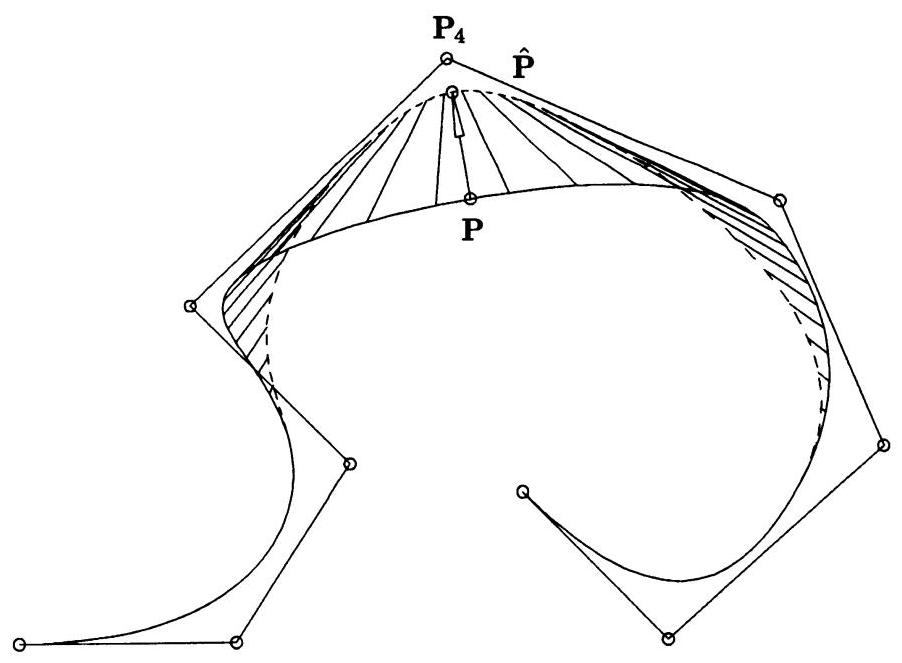
\includegraphics[max width=0.8\textwidth]{images/0193ba0d-ab19-7138-9798-cb281ce60de0_530_318_1327_902_663_0.jpg}
\end{center}
\hspace*{3em} 

图 11.11. 通过改变权重 \({w}_{4} = {0.2}\) ，将曲线在 \({t}_{4} = u = {0.52}\) 处拉动 \(d = {0.075}\) 的距离朝向 \({\mathbf{P}}_{4}\) ；计算出的新权重为 \({\widehat{w}}_{4} = {2.45}\) 。注意由于权重变化而产生的曲线段的透视变换。

\begin{itemize}
\item 与控制点重新定位的情况一样，结点插入可以在这里用于限制曲线变化的范围，使其位于两个用户指定的曲线点之间。
\end{itemize}

图 11.13 显示了增量拉动的一个例子。注意权重的指数变化。



\subsection{两个相邻曲线权重的修改}

现在我们考虑同时修改两个邻近曲线的权重， \({w}_{k}\) 和 \({w}_{k + 1}\) 。这样的修改会将曲线拉向(或推离)控制多边形的边 \({\mathbf{P}}_{k}{\mathbf{P}}_{k + 1}\) 。固定 \(\bar{u} \in  \left\lbrack  {{u}_{k + 1},{u}_{k + p + 1}}\right)\) ，设 \(\mathbf{P} =\)  \(\mathbf{C}\left( {\bar{u};{w}_{k},{w}_{k + 1}}\right)\) 并定义

\[
\mathbf{R} = \mathbf{C}\left( {\bar{u};{w}_{k} = {w}_{k + 1} = 0}\right)  \tag{11.26}
\]

(见图 11.14)。然后 \(\mathbf{P}\) 可以表示为

\[
\mathbf{P} = \left( {1 - {a}_{k} - {a}_{k + 1}}\right) \mathbf{R} + {a}_{k}{\mathbf{P}}_{k} + {a}_{k + 1}{\mathbf{P}}_{k + 1} \tag{11.27}
\]

权重修改 527

\begin{center}
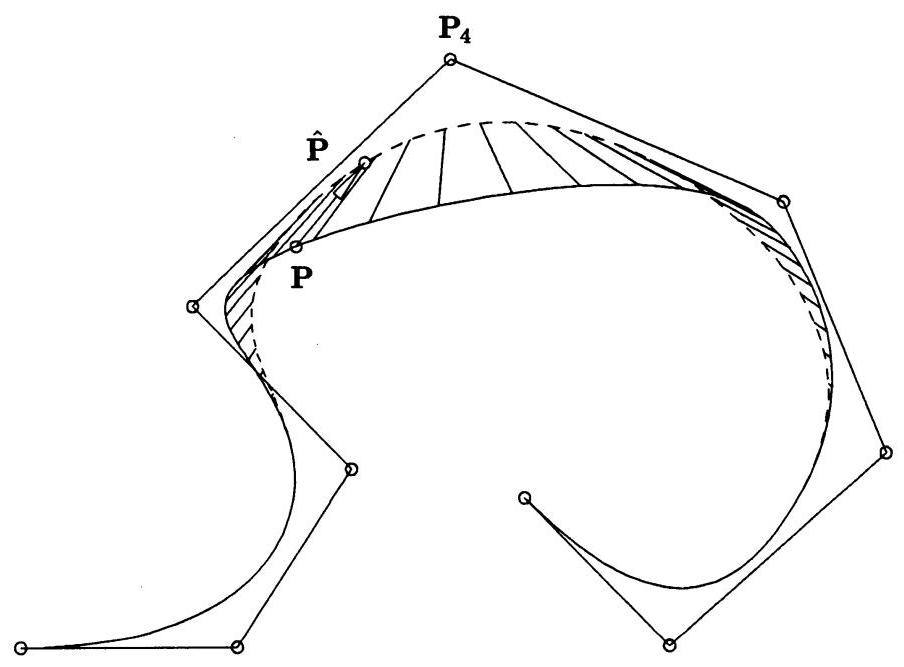
\includegraphics[max width=0.8\textwidth]{images/0193ba0d-ab19-7138-9798-cb281ce60de0_531_318_1360_904_667_0.jpg}
\end{center}
\hspace*{3em} 

图 11.12。通过改变权重 \({w}_{4} = {0.2}\) ，将曲线在 \(u = {0.46}\) 处拉向 \({\mathbf{P}}_{4}\) 的距离 \(d = {0.075}\) ；计算得到的新权重为 \({\widehat{w}}_{4} = {0.97}\) 。

\begin{center}
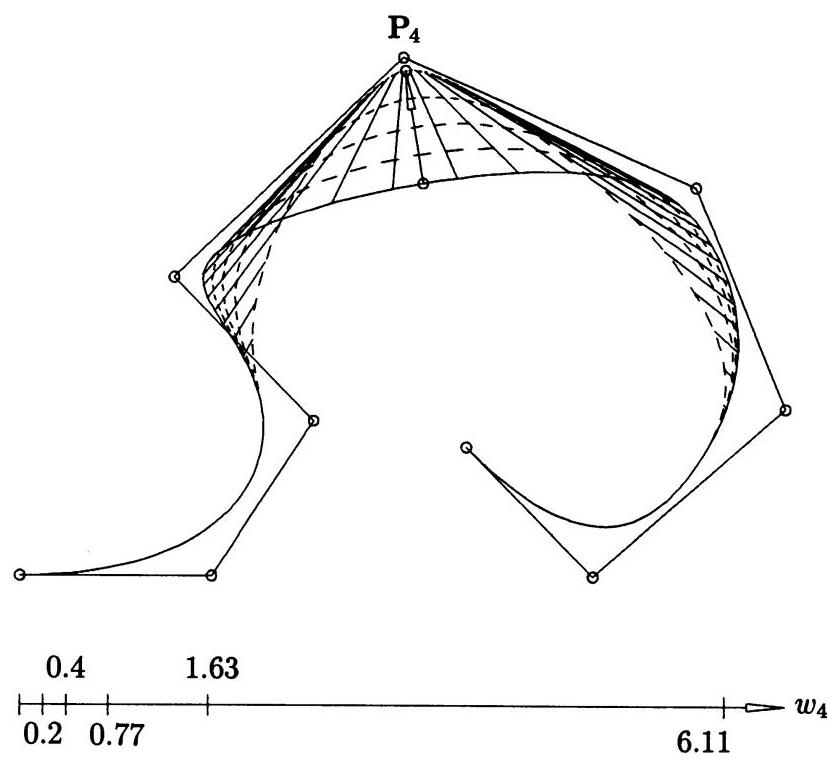
\includegraphics[max width=0.7\textwidth]{images/0193ba0d-ab19-7138-9798-cb281ce60de0_532_348_238_836_764_0.jpg}
\end{center}
\hspace*{3em} 

图 11.13。通过改变权重 \({w}_{4} = {0.2}\) ，以相等增量 \(\Delta  = {0.022}\) 将曲线在 \({t}_{4} = u = {0.52}\) 处拉向 \({\mathbf{P}}_{4}\) ；计算得到的新权重为 \({\widehat{w}}_{4} =\)  \(\{ {0.4},{0.77},{1.63},{6.11}\}\) 。

\begin{center}
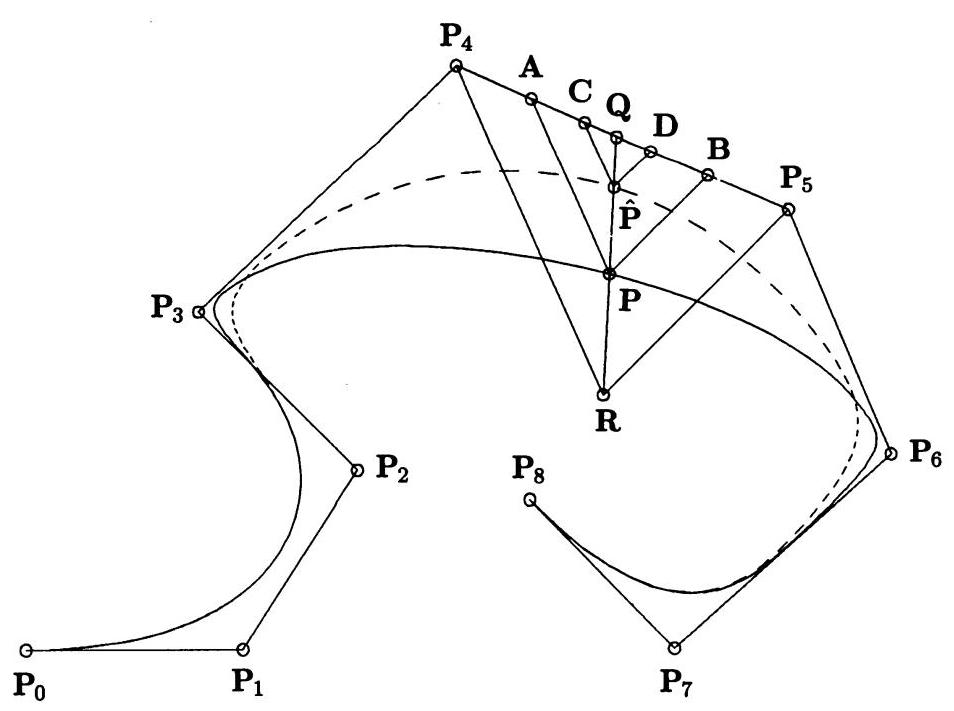
\includegraphics[max width=0.8\textwidth]{images/0193ba0d-ab19-7138-9798-cb281ce60de0_532_291_1321_954_711_0.jpg}
\end{center}
\hspace*{3em} 

图 11.14。通过同时改变 \({w}_{4}\) 和 \({w}_{5}\) ，同时向 \({\mathbf{P}}_{4}\) 和 \({\mathbf{P}}_{5}\) 拉动。

与

\[
{a}_{k} = \frac{{N}_{k,p}\left( \bar{u}\right) {w}_{k}}{\mathop{\sum }\limits_{{i = 0}}^{n}{N}_{i,p}\left( \bar{u}\right) {w}_{i}}\;{a}_{k + 1} = \frac{{N}_{k + 1,p}\left( \bar{u}\right) {w}_{k + 1}}{\mathop{\sum }\limits_{{i = 0}}^{n}{N}_{i,p}\left( \bar{u}\right) {w}_{i}} \tag{11.28}
\]

方程 (11.27) 表示 \(\mathbf{P}\) 位于重心坐标系 \(\left( {{\mathbf{{RP}}}_{k}{\mathbf{P}}_{k + 1}}\right)\) 的平面上(不熟悉重心坐标的读者应参考 Boehm 和 Prautzsch [Boeh94] 或 Farin [Fari93])。现在假设 \(\mathbf{P}\) 移动到一个新位置 \(\widehat{\mathbf{P}}\) 。我们必须确定新的权重 \({\widehat{w}}_{k}\) 和 \({\widehat{w}}_{k + 1}\) ，以导致所需的移动。根据方程 (11.27)， \(\widehat{\mathbf{P}}\) 可以表示为

\[
\widehat{\mathbf{P}} = \left( {1 - {\widehat{a}}_{k} - {\widehat{a}}_{k + 1}}\right) \mathbf{R} + {\widehat{a}}_{k}{\mathbf{P}}_{k} + {\widehat{a}}_{k + 1}{\mathbf{P}}_{k + 1} \tag{11.29}
\]

与

\[
{\widehat{a}}_{k} = \frac{{N}_{k,p}\left( \bar{u}\right) {\widehat{w}}_{k}}{d}\;{\widehat{a}}_{k + 1} = \frac{{N}_{k + 1,p}\left( \bar{u}\right) {\widehat{w}}_{k + 1}}{d}
\]

where

\[
d = \mathop{\sum }\limits_{{i \neq  k,k + 1}}{N}_{i,p}\left( \bar{u}\right) {w}_{i} + {N}_{k,p}\left( \bar{u}\right) {\widehat{w}}_{k} + {N}_{k + 1,p}\left( \bar{u}\right) {\widehat{w}}_{k + 1}
\]

如果 \({\widehat{w}}_{k}\) 和 \({\widehat{w}}_{k + 1}\) 表达为

\[
{\widehat{w}}_{k} = {\beta }_{k}{w}_{k}\;{\widehat{w}}_{k + 1} = {\beta }_{k + 1}{w}_{k + 1} \tag{11.30}
\]

那么经过一些操作可以得到

\[
{\beta }_{k} = \frac{1 - {a}_{k} - {a}_{k + 1}}{{a}_{k}}/\frac{1 - {\widehat{a}}_{k} - {\widehat{a}}_{k + 1}}{{\widehat{a}}_{k}}
\]

\[
{\beta }_{k + 1} = \frac{1 - {a}_{k} - {a}_{k + 1}}{{a}_{k + 1}}/\frac{1 - {\widehat{a}}_{k} - {\widehat{a}}_{k + 1}}{{\widehat{a}}_{k + 1}} \tag{11.31}
\]

方程 (11.27)-(11.31) 导致了一种简单的几何方法来求解未知数 \({\beta }_{k}\) 和 \({\beta }_{k + 1}\) ，从而从 \({w}_{k}\) 和 \({w}_{k + 1}\) 中获得 \({\widehat{w}}_{k}\) 和 \({\widehat{w}}_{k + 1}\) 。由于 \({a}_{k},{a}_{k + 1},{\widehat{a}}_{k}\) 和 \({\widehat{a}}_{k + 1}\) 是相对于 \(\mathbf{R},{\mathbf{P}}_{k}\) 和 \({\mathbf{P}}_{k + 1}\) 的重心坐标，它们可以通过(见图 11.14)表示。

\[
{a}_{k} = \frac{\left| \mathbf{B} - {\mathbf{P}}_{k + 1}\right| }{\left| {\mathbf{P}}_{k + 1} - {\mathbf{P}}_{k}\right| }\;{a}_{k + 1} = \frac{\left| \mathbf{A} - {\mathbf{P}}_{k}\right| }{\left| {\mathbf{P}}_{k + 1} - {\mathbf{P}}_{k}\right| }
\]

\[
{\widehat{a}}_{k} = \frac{\left| \mathbf{D} - {\mathbf{P}}_{k + 1}\right| }{\left| {\mathbf{P}}_{k + 1} - {\mathbf{P}}_{k}\right| }\;{\widehat{a}}_{k + 1} = \frac{\left| \mathbf{C} - {\mathbf{P}}_{k}\right| }{\left| {\mathbf{P}}_{k + 1} - {\mathbf{P}}_{k}\right| } \tag{11.32}
\]

其中 \(\mathbf{A},\mathbf{B},\mathbf{C}\) 和 \(\mathbf{D}\) 是沿 \({\mathbf{P}}_{k}{\mathbf{P}}_{k + 1}\) 的点，使得 \(\mathbf{{PA}}\) 和 \(\widehat{\mathbf{P}}\mathbf{C}\) 与 \(\mathbf{R}{\mathbf{P}}_{k}\) 平行，而 \(\mathbf{{PB}}\) 和 \(\widehat{\mathbf{P}}\mathbf{D}\) 与 \(\mathbf{R}{\mathbf{P}}_{k + 1}\) 平行。为了使 \({a}_{k},\bar{u}\) 不为零，必须在 \(\left\lbrack  {{u}_{k},{u}_{k + p + 1}}\right)\) 内；同样，对于不为零的 \({a}_{k + 1}\bar{u}\) ，必须在 \(\left\lbrack  {{u}_{k + 1},{u}_{k + p + 2}}\right)\) 内。如果选择 \(\mathbf{P}\) 使得 \(\bar{u}\) 在这些区间的交集内，则 \({a}_{k}\) 和 \({a}_{k + 1}\) 都不为零，因此 \(\widehat{\mathbf{P}}\) 可以放置在三角形 \(\mathbf{R}{\mathbf{P}}_{k}{\mathbf{P}}_{k + 1}\) 内的任何位置。然而，如果 \(\bar{u} \in  \left\lbrack  {{u}_{k},{u}_{k + 1}}\right)\) ，则 \({a}_{k + 1} =\) 0，方程 (11.27) 退化为

\[
\mathbf{P} = \left( {1 - {a}_{k}}\right) \mathbf{R} + {a}_{k}{\mathbf{P}}_{k} \tag{11.33}
\]

即，同时修改退化为单一权重修改。

图 11.15 和 11.16 显示了同时的推拉。注意，在图 11.15 中曲线变化是令人愉悦且对称的，而在图 11.16 中则不是。这是因为在图 11.15 中，运动沿着由 \(\mathbf{R}\) 和初始 \(\mathbf{P} = \mathbf{C}\left( {\bar{u};{w}_{k}}\right)\) 定义的线进行。在这种情况下，我们有

\[
\frac{{\widehat{a}}_{k}}{{a}_{k}} = \frac{{\widehat{a}}_{k + 1}}{{a}_{k + 1}}
\]

这意味着 \({\beta }_{k} = {\beta }_{k + 1}\) 和

\[
\frac{{w}_{k}}{{w}_{k + 1}} = \frac{{\widehat{w}}_{k}}{{\widehat{w}}_{k + 1}}
\]

也就是说，权重的比率被保留。

同时权重修改的用户界面可能如下所示。设计师选择一个控制多边形边， \({\mathbf{P}}_{k}{\mathbf{P}}_{k + 1}\) 。系统计算相应的节点， \({t}_{k}\) 和 \({t}_{k + 1}\) ，并设置 \(\bar{u} = 1/2\left( {{t}_{k} + {t}_{k + 1}}\right)\) 。然后系统计算 \(\mathbf{R},\mathbf{P} = \mathbf{C}\left( \bar{u}\right)\) 和 \(\mathbf{Q}\) ( \(\mathbf{{RP}}\) 与 \({\mathbf{P}}_{k}{\mathbf{P}}_{k + 1}\) 的交点；见

\begin{center}
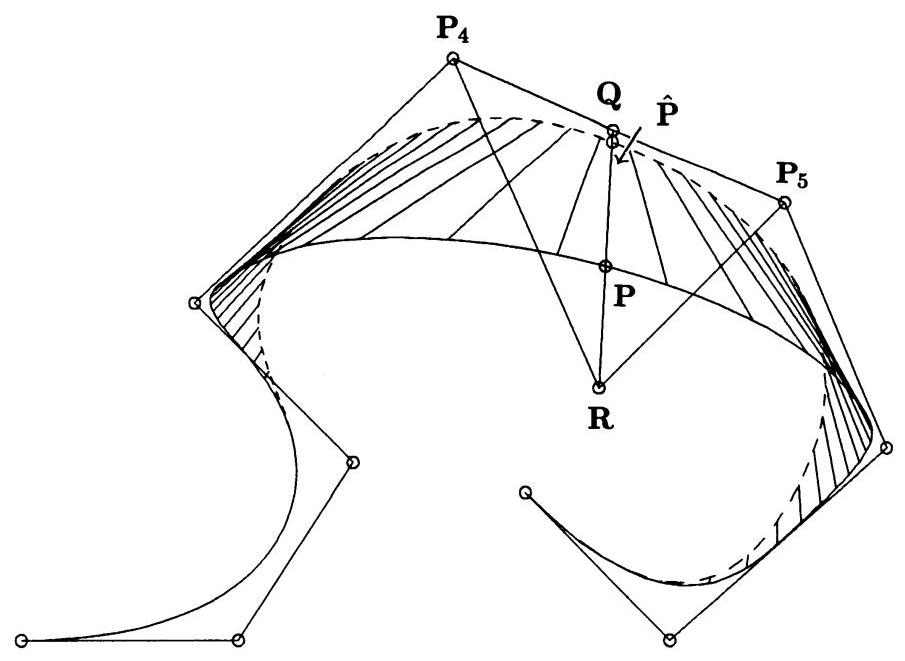
\includegraphics[max width=0.8\textwidth]{images/0193ba0d-ab19-7138-9798-cb281ce60de0_534_312_1334_905_661_0.jpg}
\end{center}
\hspace*{3em} 

图 11.15。在 \(u = 1/2\left( {{t}_{4} + {t}_{5}}\right)  = {0.608}\) 处以距离 \(d = {0.088}\) 沿着 \(\mathbf{{RQ}}\) 方向进行同时拉动，通过改变 \({w}_{4} = {w}_{5} = {0.05}\) ；新的权重为 \({\widehat{w}}_{4} = {\widehat{w}}_{5} = {1.23}\) 。曲线的变化既不是透视的也不是平行的。

\begin{center}
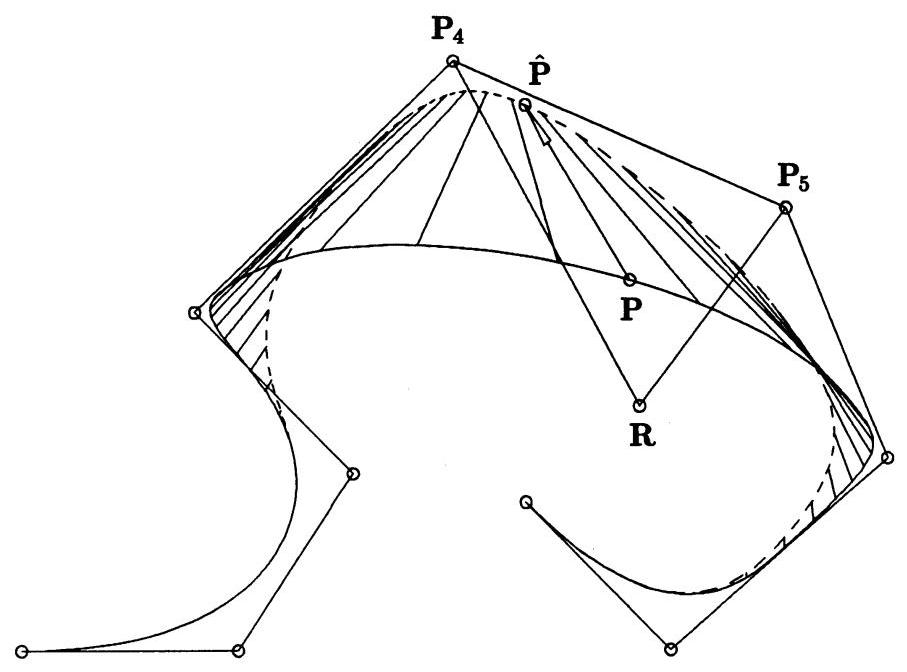
\includegraphics[max width=0.8\textwidth]{images/0193ba0d-ab19-7138-9798-cb281ce60de0_535_312_255_907_672_0.jpg}
\end{center}
\hspace*{3em} 

图 11.16。在 \(u = {0.612}\) 处以距离 \(d = {0.088}\) 沿着与 RQ 不同的方向进行同时拉动，通过改变 \({w}_{4} = {w}_{5} = {0.05}\) ；新的权重为 \({\widehat{w}}_{4} = {1.89}\) 和 \({\widehat{w}}_{5} = {0.48}\) 。

图 11.14。这些组件，包括线段 \(\mathbf{{RQ}}\) ，被绘制在屏幕上。设计师现在可以交互式地重新定位 \(\mathbf{P}\) 沿着线 \(\mathbf{{RQ}}\) ，同时系统计算新的权重并重新绘制受影响的曲线段。当然，设计师应该能够覆盖默认值 \(\bar{u}\) 和默认线段 \(\mathbf{{RQ}}\) 。

另一种情况是允许设计师选择曲线点 \(\mathbf{P}\) (从而 \(\bar{u}\) )，然后系统通过找到两个节点 \({t}_{k}\) 和 \({t}_{k + 1}\) 来选择多边形边 \({\mathbf{P}}_{k}{\mathbf{P}}_{k + 1}\) ，使得 \({t}_{k} < \bar{u} < {t}_{k + 1}\) 。然而，如果 \(\bar{u}\) 等于或接近一个节点，这将是有问题的，因为如果任意选择一个多边形边，推拉效果是非对称的。在这种情况下，可以插入一个节点 \(\widehat{u}\) ，将 \(\bar{u}\) 放置在两个节点之间的中间位置。具体来说

\[
\bar{u} = \frac{1}{2}\left( {{\widehat{t}}_{k} + {\widehat{t}}_{k + 1}}\right)
\]

\[
= \frac{1}{2p}\left( {{u}_{k + 1} + \cdots  + {u}_{k + p - 1} + \widehat{u} + {u}_{k + 2} + \cdots  + {u}_{k + p} + \widehat{u}}\right)
\]

\[
= \frac{1}{2p}\left( {{u}_{k + 1} + {u}_{k + p} + 2\widehat{u} + 2\mathop{\sum }\limits_{{j = k + 2}}^{{k + p - 1}}{u}_{j}}\right)
\]

这意味着

\[
\widehat{u} = p\bar{u} - \frac{1}{2}\left( {{u}_{k + 1} + {u}_{k + p}}\right)  - \mathop{\sum }\limits_{{j = 2}}^{{p - 1}}{u}_{k + j}
\]

然而，我们提醒读者， \(\widehat{u}\) 可能已经是一个结；此外，生成的新多边形腿 \({\mathbf{P}}_{k}{\mathbf{P}}_{k + 1}\) 可能非常接近 \(\mathbf{P} = \mathbf{C}\left( \bar{u}\right)\) ，在这种情况下，可用的拉伸长度非常有限。

最后，请注意我们之前假设修改权重的两个控制点是相邻的。这是因为这样可以产生令人满意的结果，并且通常是所期望的。然而，方程 (11.27)-(11.32) 的推导并没有利用这一假设。事实上，如果选择 \({\mathbf{P}}_{r}\) 和 \({\mathbf{P}}_{s}\) ，那么唯一的要求是 \(\bar{u} \in  \left\lbrack  {{u}_{r},{u}_{r + p + 1}}\right)\) 和 \(\bar{u} \in  \left\lbrack  {{u}_{s},{u}_{s + p + 1}}\right)\) ，以便重心坐标 \({a}_{r}\) 和 \({a}_{s}\) 不会消失。有关此情况的更多细节，请参见 [Pieg89c]。


\subsection{单表面权重的修改}

修改单个表面权重 \({w}_{k,\ell }\) 类似于曲线情况。假设 \(\bar{u} \in  \left\lbrack  {{u}_{k},{u}_{k + p + 1}}\right)\) 和 \(\bar{v} \in  \left\lbrack  {{v}_{\ell },{v}_{\ell  + q + 1}}\right)\) ，并定义

\[
\mathbf{R} = \mathbf{S}\left( {\bar{u},\bar{v};{w}_{k,\ell } = 0}\right)
\]

\[
\mathbf{M} = \mathbf{S}\left( {\bar{u},\bar{v};{w}_{k,\ell } = 1}\right)
\]

\[
\mathbf{P} = \mathbf{S}\left( {\bar{u},\bar{v};{w}_{k,\ell } \neq  0,1}\right)  \tag{11.35}
\]

然后 \(\mathbf{M}\) 和 \(\mathbf{P}\) 可以表示为

\[
\mathbf{M} = \left( {1 - s}\right) \mathbf{R} + s{\mathbf{P}}_{k,\ell }
\]

\[
\mathbf{P} = \left( {1 - t}\right) \mathbf{R} + t{\mathbf{P}}_{k,\ell } \tag{11.36}
\]

其中

\[
s = \frac{{N}_{k,p}\left( \bar{u}\right) {N}_{\ell ,q}\left( \bar{v}\right) }{\mathop{\sum }\limits_{{i,j \neq  k,\ell }}{N}_{i,p}\left( \bar{u}\right) {N}_{j,q}\left( \bar{v}\right) {w}_{i,j} + {N}_{k,p}\left( \bar{u}\right) {N}_{\ell ,q}\left( \bar{v}\right) }
\]

\[
t = \frac{{N}_{k,p}\left( \bar{u}\right) {N}_{\ell ,q}\left( \bar{v}\right) {w}_{k,\ell }}{\mathop{\sum }\limits_{{i = 0}}^{n}\mathop{\sum }\limits_{{j = 0}}^{m}{N}_{i,p}\left( \bar{u}\right) {N}_{j,q}\left( \bar{v}\right) {w}_{i,j}} = {R}_{k,\ell }\left( {\bar{u},\bar{v}}\right)  \tag{11.37}
\]

\(\left( {i,j \neq  k,\ell \text{ means exclude the }\left( {k,\ell }\right) \text{ th term. }}\right)\) 使用方程 (11.36) 和 (11.37)，可以得到交叉比

\[
{w}_{k,\ell } = \frac{1 - s}{\mathrm{\;s}}/\frac{1 - t}{t} = \frac{{\mathbf{P}}_{k,\ell }\mathbf{M}}{\mathbf{{RM}}}/\frac{{\mathbf{P}}_{k,\ell }\mathbf{P}}{\mathbf{{RP}}} \tag{11.38}
\]

方程 (11.35)-(11.38) 意味着

\begin{itemize}
\item 当 \({w}_{k,\ell }\) 增加(减少)时， \(t\) 增加(减少)，因此表面被拉向(推离) \({\mathbf{P}}_{k,\ell }\) ；
\end{itemize}

\begin{itemize}
\item \(\mathbf{P}\) 沿着通过 \({\mathbf{P}}_{k,\ell }\) 的直线段移动；因此，对 \({w}_{k,\ell }\) 的修改以可预测的方式改变表面；
\end{itemize}

\begin{itemize}
\item 当 \(\mathbf{P}\) 接近时， \({\mathbf{P}}_{k,\ell },t\) 接近 1，而 \({w}_{k,\ell }\) 趋向于无穷大。
\end{itemize}

最后，如果 \(\mathbf{P}\) 要移动到新位置 \(\widehat{\mathbf{P}}\) 和 \(d = \left| {\mathbf{P} - \widehat{\mathbf{P}}}\right|\) ，则所需的新权重值 \({\widehat{w}}_{k,\ell }\) 为

\[
{\widehat{w}}_{k,\ell } = {w}_{k,\ell }\left( {1 \pm  \frac{d}{{R}_{k,\ell }\left( {\bar{u},\bar{v}}\right) \left( {{\mathbf{P}}_{k,\ell }\mathbf{P} \mp  d}\right) }}\right)  \tag{11.39}
\]

当出现 \(\pm\) 或 \(\mp\) 时，拉动操作的情况下取上面的符号，而推送操作的情况下取下面的符号 [Pieg89d]。

单个表面权重的修改用户界面可以以类似于曲线的方式实现。设计师可以选择一个现有的控制点或一个或两个位于控制网边缘的点；如果是两个，则它们必须位于控制网的一个四边形上，一个在 \(u\) 方向的边上，另一个在 \(v\) 方向的边上。如果没有选择现有的控制点，则使用逆节点插入来获得 \({\mathbf{P}}_{k,\ell }\) 。从那里，过程与曲线修改相同。与之前提到的五个关于曲线权重修改的备注类似的声明也适用于表面权重修改。图 11.17 说明了表面推送。

\begin{center}
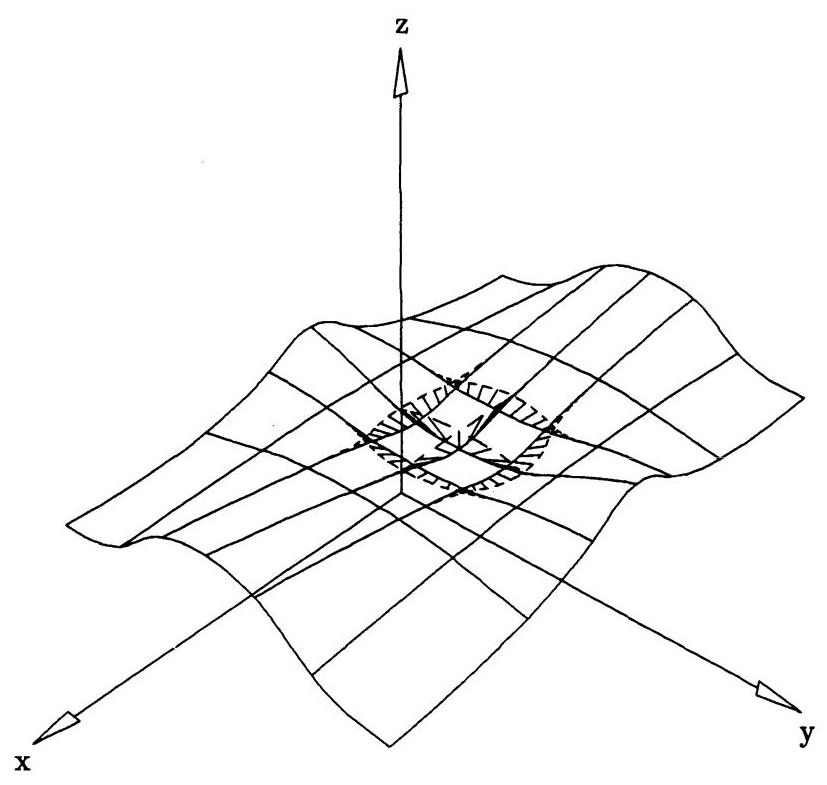
\includegraphics[max width=0.7\textwidth]{images/0193ba0d-ab19-7138-9798-cb281ce60de0_537_354_1252_827_785_0.jpg}
\end{center}
\hspace*{3em} 

图 11.17. 在 \(u = v = {0.55}\) 处向 \({\mathbf{P}}_{4,3}\) 推送表面，距离 \(d = 1\) ；注意表面形状的透视变化。


\section{形状操作符}
在此定义的形状操作符是用于粗略雕刻曲线和表面的工具。它们的操作如下:

1. 指定一个局部曲线段或表面区域，在其中进行形状修改；然后使用节点细化在局部引入更多控制点；

2. 根据各种参数和/或函数重新定位对指定段或区域影响局部的控制点；

3. 对局部段或区域应用在指定容差内的节点移除，以减少定义控制点的数量。

我们在这里介绍三种操作符:扭曲、展平和弯曲。文献中可以找到其他类似的操作符，例如，拉伸、扭转和渐变 [Barr83; Cobb84]。我们强调我们的算法完全基于几何；它们不考虑材料的物理特性或弹性和塑性理论。

在介绍操作符之前，我们提到一些与节点细化和移除步骤相关的问题。细化的方法和程度会影响应用形状操作符的结果。因此，尽管设计者应该免于细节，但他必须能够控制细化的程度。假设 \(\left\lbrack  {{u}_{s},{u}_{e}}\right\rbrack\) 是一个感兴趣的曲线段。如果 \({u}_{s}\) 和 \({u}_{e}\) 还不是节点，则将其插入。将 \(n\) 额外节点递归插入到 \(\left\lbrack  {{u}_{s},{u}_{e}}\right\rbrack\) 中最长节点跨度的中点是一个好的方法。这往往会生成大致均匀间隔的节点，并且希望(但不一定)控制点也会大致均匀间隔。现在，如果 \({u}_{s}\) 和 \({u}_{e}\) 是定义最终细化区间限制的节点(注意 \(e\) 在细化过程中会变化)，那么可以在不修改 \(\left\lbrack  {{u}_{s},{u}_{e}}\right\rbrack\) 外部曲线的情况下重新定位以下控制点。

\[
{\mathbf{P}}_{s},\ldots ,{\mathbf{P}}_{e - p - 1} \tag{11.40}
\]

其中 \(p\) 是曲线的度数。在形状操作之后，节点移除通常会去除许多插入的节点。如果曲线不应在 \(\left\lbrack  {{u}_{s},{u}_{e}}\right\rbrack\) 外部被修改，则只有以下节点是移除的候选者。

\[
{u}_{i}\;i = s + \frac{p}{2},\ldots ,e - \frac{p}{2} - 1\;\text{ if }p\text{ is even }
\]

\[
{u}_{i}\;i = s + \frac{p + 1}{2},\ldots ,e - \frac{p + 1}{2}\;\text{ if }p\text{ is odd } \tag{11.41}
\]



\subsection{变形}

扭曲是一种工具，可以用来相对任意地变形曲线的局部段或表面上的区域。首先考虑曲线扭曲，它是通过基于公式的控制点重新定位来实现的。

\[
{\widehat{\mathbf{P}}}_{i} = {\mathbf{P}}_{i} + {fd}\mathbf{W} \tag{11.42}
\]

一般来说， \(f\) 是一个函数， \(d\) 是一个常数，而 \(\mathbf{W}\) 可以是一个函数或一个常数。 \(f\) 控制变形形状， \(d\) 是控制点移动的上限(因此也是变形距离的上限)，而 \(\mathbf{W}\) 给出了变形的方向。设计师通常通过选择曲线点 \(\mathbf{C}\left( {u}_{s}\right)\) 和 \(\mathbf{C}\left( {u}_{e}\right)\) 来确定变形的程度。曲线变形限制在这个区间内。一个有用的变形函数为

\[
f\left( t\right)  = \frac{{R}_{3,3}\left( t\right) }{{R}_{\max }} \tag{11.43}
\]

其中 \({R}_{\max } = {R}_{3,3}\left( {1/2}\right)\) 和 \({R}_{3,3}\left( t\right)\) 是有理立方 B 样条基函数

\[
{R}_{3,3}\left( t\right)  = \frac{{N}_{3,3}\left( t\right) {w}_{3}}{\mathop{\sum }\limits_{{i = 0}}^{6}{N}_{i,3}\left( t\right) {w}_{i}} \tag{11.44}
\]

由节点向量定义

\[
T = \left\{  {0,0,0,0,\frac{1}{4},\frac{1}{2},\frac{3}{4},1,1,1,1}\right\}   \tag{11.45}
\]

和权重

\[
{w}_{i} = \left\{  {1,1,1,{w}_{3},1,1,1}\right\}
\]

图 11.18 显示了 \(f\left( t\right)\) 对于 \({w}_{3}\) 的几个不同值。显然，这种形式的函数适合于拉出一个隆起或在曲线上推入一个凹陷。现在假设 \({w}_{3}\) 是固定的，设计师指定一个最大变形距离 \(d\) 。变形方向 \(\mathbf{W}\) 仍需指定。合理的选择包括:

\begin{center}
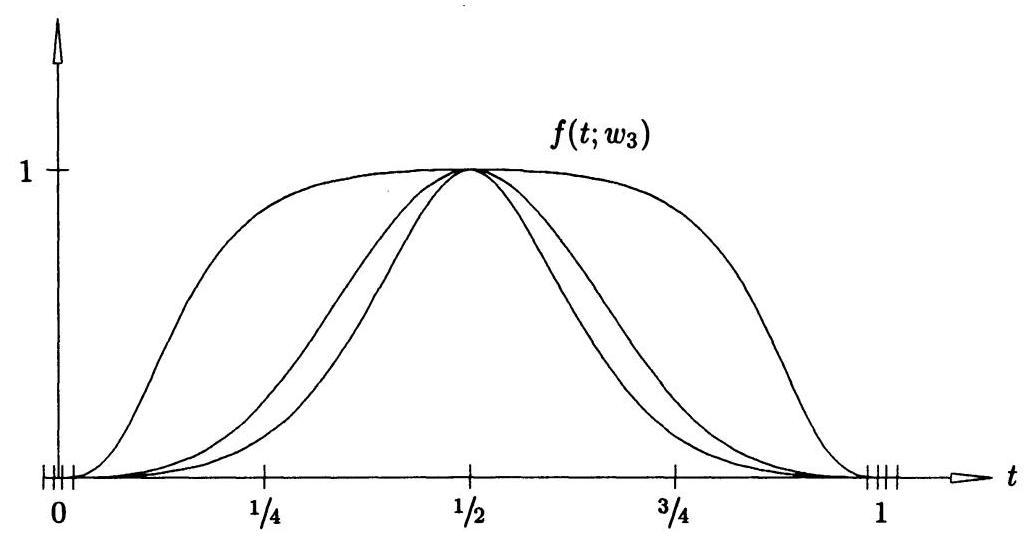
\includegraphics[max width=0.9\textwidth]{images/0193ba0d-ab19-7138-9798-cb281ce60de0_539_249_1517_1030_538_0.jpg}
\end{center}
\hspace*{3em} 

图 11.18. 使用有理基函数 \({R}_{3,3}\left( {t;{w}_{3}}\right)\) 和 \({w}_{3} = \left\{  {1/5,1,{30}}\right\}\) 的变形函数。

\begin{itemize}
\item 由以下给出的变量方向
\end{itemize}

\[
\mathbf{W}\left( t\right)  =  \pm  \mathbf{N}\left( {u\left( t\right) }\right)  \tag{11.46}
\]

其中 \(\mathbf{N}\left( u\right)\) 是 \(\mathbf{C}\left( u\right)\) 和 \(u\left( t\right)  = \left( {{u}_{e} - {u}_{s}}\right) t + {u}_{s}\) 的单位法向量；- 由以下给出的恒定方向

\[
\mathbf{W} =  \pm  \mathbf{N}\left( {\frac{1}{2}\left( {{u}_{s} + {u}_{e}}\right) }\right)  \tag{11.47}
\]

区间 \(\left\lbrack  {{u}_{s},{u}_{e}}\right\rbrack\) 现在被细化，产生控制点 \({\mathbf{P}}_{i},i = s,\ldots ,e - p - 1\) (方程 [11.40])，这些控制点可以根据方程 (11.42) 进行重新定位。为了应用该方程，我们必须为每个 \({\mathbf{P}}_{i},i = s,\ldots ,e - p - 1\) 指定一个参数 \({t}_{i}\) 。设 \(\delta\) 表示从 \({\mathbf{P}}_{s - 1}\) 到 \({\mathbf{P}}_{e - p}\) 的控制多边形沿线的总累积弦长。用 \({t}_{i}\) 表示从 \({\mathbf{P}}_{s - 1}\) 到 \({\mathbf{P}}_{i}\) 的累积弦长，经过 \(\delta\) 归一化。注意到 \(0 \leq  {t}_{i} \leq  1\) 对于 \(s \leq  i \leq  e - p - 1\) 。然后 \({\mathbf{P}}_{i}\) 被重新定位为

\[
{\widehat{\mathbf{P}}}_{i} = {\mathbf{P}}_{i} + f\left( {t}_{i}\right) d\mathbf{W}\left( {t}_{i}\right) \;i = s,\ldots ,e - p - 1 \tag{11.48}
\]

最后，按照之前讨论的内容，对区间应用节点移除。

图 11.19a-11.19d 显示了曲线扭曲的步骤。在图 11.19a 中，选择了曲线段 \(\left\lbrack  {\mathbf{C}\left( {u}_{s}\right) ,\mathbf{C}\left( {u}_{e}\right) }\right\rbrack\) 、(恒定)方向 \(\mathbf{W}\) 和距离 \(d\) 。图 11.19b 显示了节点细化后的曲线。局部控制点被重新定位，如图 11.19c 所示。图 11.19d 描绘了应用节点移除后的最终曲线。

\begin{center}
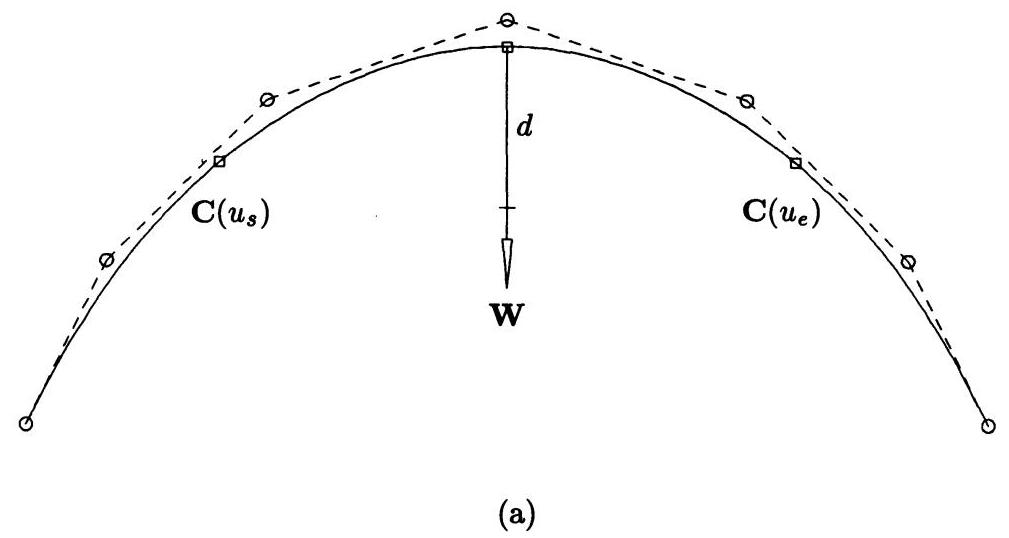
\includegraphics[max width=0.9\textwidth]{images/0193ba0d-ab19-7138-9798-cb281ce60de0_540_260_1491_1009_538_0.jpg}
\end{center}
\hspace*{3em} 

图 11.19. 曲线扭曲。 (a) 原始曲线，跨度为 \(\left\lbrack  {\mathbf{C}\left( {u}_{s}\right) ,\mathbf{C}\left( {u}_{e}\right) }\right\rbrack\) ，将在方向 \(\mathbf{W}\) 上扭曲距离 \(d\) ；(b) 细化后的曲线跨度；(c) 重新定位的控制点；(d) 移除的节点。

\begin{center}
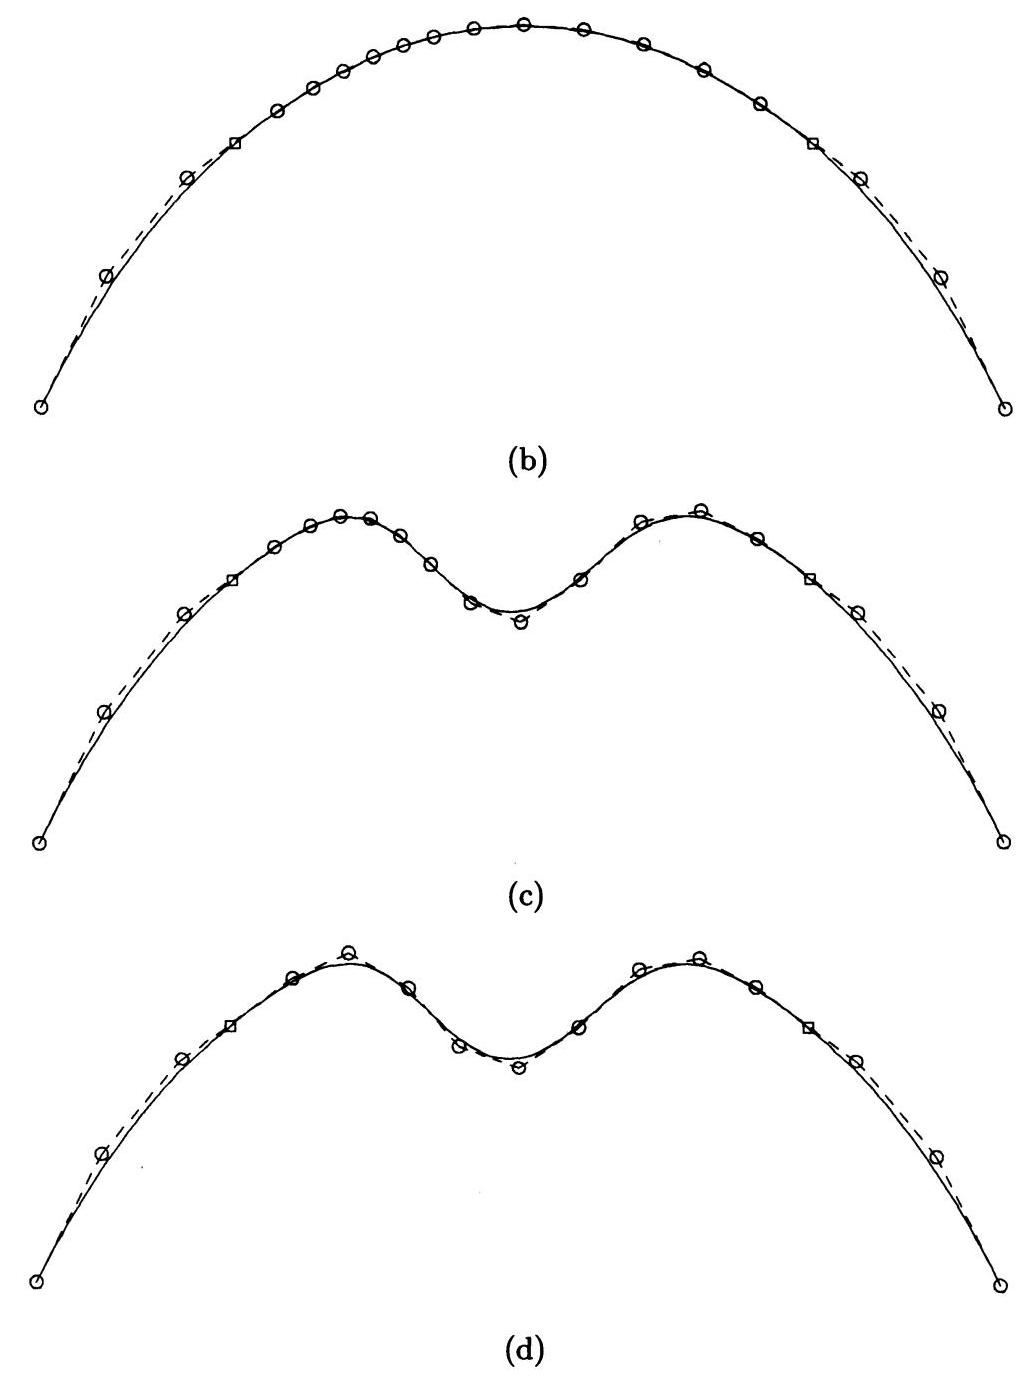
\includegraphics[max width=0.9\textwidth]{images/0193ba0d-ab19-7138-9798-cb281ce60de0_541_249_262_1033_1377_0.jpg}
\end{center}
\hspace*{3em} 

图 11.19. (续。)

改变定义参数的效果在图 11.20a-11.20c 中得以展示。在图 11.20a 中，使用不同的权重来“平方”扭曲区域。图 11.20b 显示了在保持权重和距离不变的情况下，改变扭曲方向的效果。最后，在图 11.20c 中，应用不同的距离来控制扭曲的幅度。

我们通过以下几点总结曲线扭曲:

\begin{itemize}
\item 显然，几乎任何形状和幅度的扭曲都是可能的；只需适当地定义函数 \(f\left( t\right)\) 和 \(\mathbf{W}\left( t\right)\) 。图 11.21a 和 11.21b 显示了两个进一步的例子；
\end{itemize}

\begin{center}
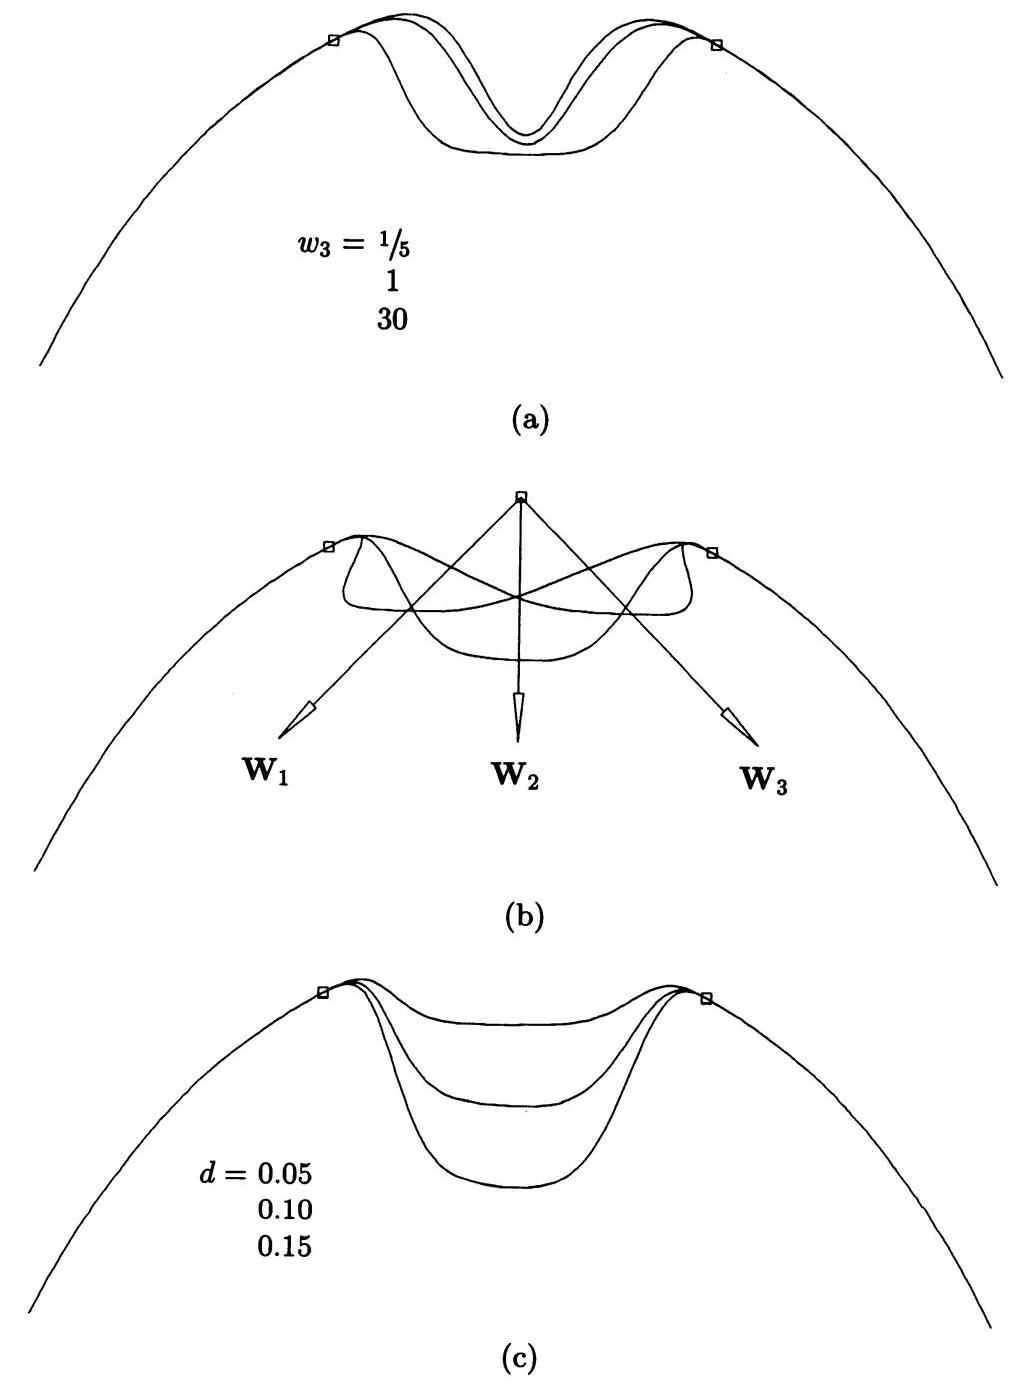
\includegraphics[max width=0.9\textwidth]{images/0193ba0d-ab19-7138-9798-cb281ce60de0_542_249_278_1026_1385_0.jpg}
\end{center}
\hspace*{3em} 

图 11.20。曲线扭曲 (a) 使用不同的权重 \({w}_{3} = \left\{  {1/5,1,{30}}\right\}\) ；(b) 使用不同的方向 \({w}_{3} = {20}\) ；(c) 使用不同的距离 \(d = \{ {0.05},{0.1},{0.15}\}\) 。

\begin{itemize}
\item 对于交互式扭曲，设计者可能希望选择一个曲线点作为扭曲的中心，然后在滑动尺度上修改幅度 \(d\) 、权重 \({w}_{3}\) 和扭曲段的范围。该段选择尽可能对称于扭曲中心，沿控制多边形的距离进行测量。交互完成后进行节点移除；节点细化必须作为预处理步骤进行(可以在整个曲线上，或者在用户指定的“最大”段上)，或者细化必须在段长度扩展时进行更新(扩展)；
\end{itemize}

\begin{itemize}
\item 而不是将 \({t}_{i}\) 计算为归一化距离，可以使用由方程 (11.4) 计算的 B 样条节点；在这种情况下，函数 \(f\) 和 \(\mathbf{W}\) 必须在区间 \(\left\lbrack  {{u}_{s},{u}_{e}}\right\rbrack\) 上进行参数化。
\end{itemize}

表面变形类似于曲线变形。我们区分两种类型，区域变形和表面曲线变形。在区域变形中，我们对非零表面积的区域应用变形函数；对于表面曲线变形，我们允许单变量变形函数沿着位于表面上的曲线滑动。

\begin{center}
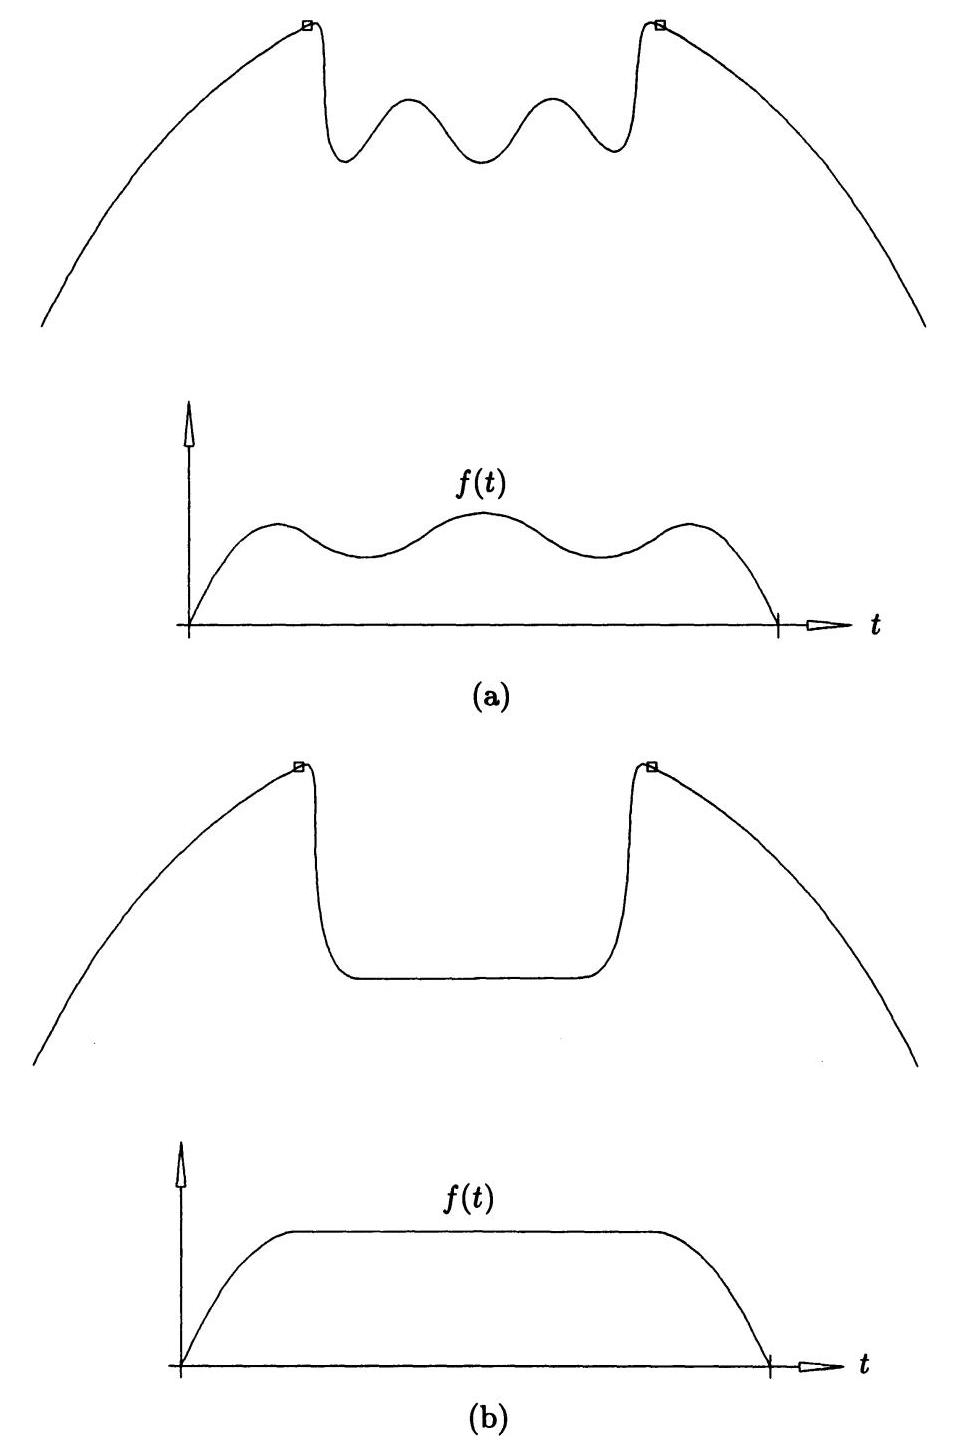
\includegraphics[max width=0.8\textwidth]{images/0193ba0d-ab19-7138-9798-cb281ce60de0_543_281_660_966_1447_0.jpg}
\end{center}
\hspace*{3em} 

图 11.21. 具有不同形状函数的曲线变形。

设 \(\mathcal{R}\) 为表面参数空间中的一个闭合区域， \(\mathbf{S}\left( {u,v}\right)\) 。示例见图 11.22a 和 11.23a。区域变形是通过重新定位控制点产生的，基于公式

\[
{\widehat{\mathbf{P}}}_{i,j} = {\mathbf{P}}_{i,j} + {fd}\mathbf{W} \tag{11.49}
\]

类似于曲线变形，节点细化应用于区域 \(\left\lbrack  {{u}_{\alpha },{u}_{\beta }}\right\rbrack   \times\)  \(\left\lbrack  {{v}_{\gamma },{v}_{\delta }}\right\rbrack\) (在图 11.22a 和 11.23a 中用虚线表示)，然后使用公式 (11.49)。节点移除在适当的区域应用(见公式 [11.41])，作为后处理步骤。每个控制点 \({\mathbf{P}}_{i,j},i = \alpha ,\ldots ,\beta  - p - 1,j = \gamma ,\ldots ,\delta  - q - 1\) 必须与一对参数 \(\left( {{s}_{i},{t}_{j}}\right)\) 相关联。这些参数用于确定哪些 \({\mathbf{P}}_{i,j}\) 需要重新定位，并评估公式 (11.49) 中的函数 \(f\) 和 \(\mathbf{W}\) 。类似于曲线变形，我们使用归一化累积弦长。特别地，我们对点集 \({\mathbf{P}}_{i,j},i = \alpha  - 1,\ldots ,\beta  - p\) 和 \(j = \gamma  - 1,\ldots ,\delta  - q\) 应用算法 A9.3。只有当 \(\left( {{u}_{i},{v}_{j}}\right)\) 位于变形区域 \(\mathcal{R}\) 中时， \({\mathbf{P}}_{i,j}\) 才会通过公式 (11.49) 重新定位，其中

\[
{u}_{i} = \left( {{u}_{\beta } - {u}_{\alpha }}\right) {s}_{i} + {u}_{\alpha }\;{v}_{j} = \left( {{v}_{\delta } - {v}_{\gamma }}\right) {t}_{j} + {v}_{\gamma }
\]

\(f\) 可以是定义在 \(\left\lbrack  {0,1}\right\rbrack   \times  \left\lbrack  {0,1}\right\rbrack\) 上的任何标量值函数。与曲线的情况一样，B样条基函数适用于拉动和推送。例如，归一化的双变量、双立方、有理 B样条基函数适用于矩形区域。

\[
f\left( {s,t}\right)  = \frac{{R}_{3,3;3,3}\left( {s,t}\right) }{{R}_{\max }} \tag{11.50}
\]

\begin{center}
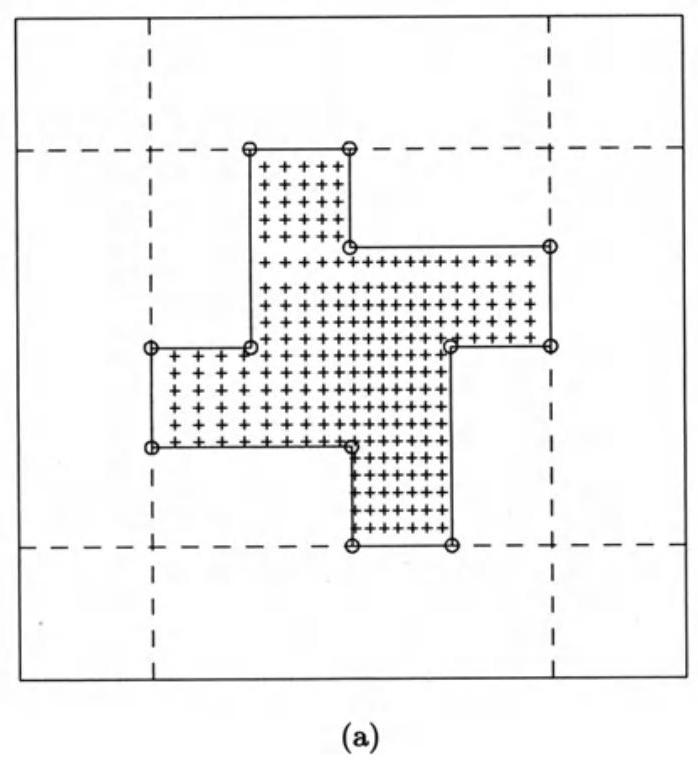
\includegraphics[max width=0.6\textwidth]{images/0193ba0d-ab19-7138-9798-cb281ce60de0_544_423_1304_698_760_0.jpg}
\end{center}
\hspace*{3em} 

图11.22. 表面区域变形。(a) 一个具有边界框和局部控制点的区域；(b) 控制点重新定位后的表面变形。

\begin{center}
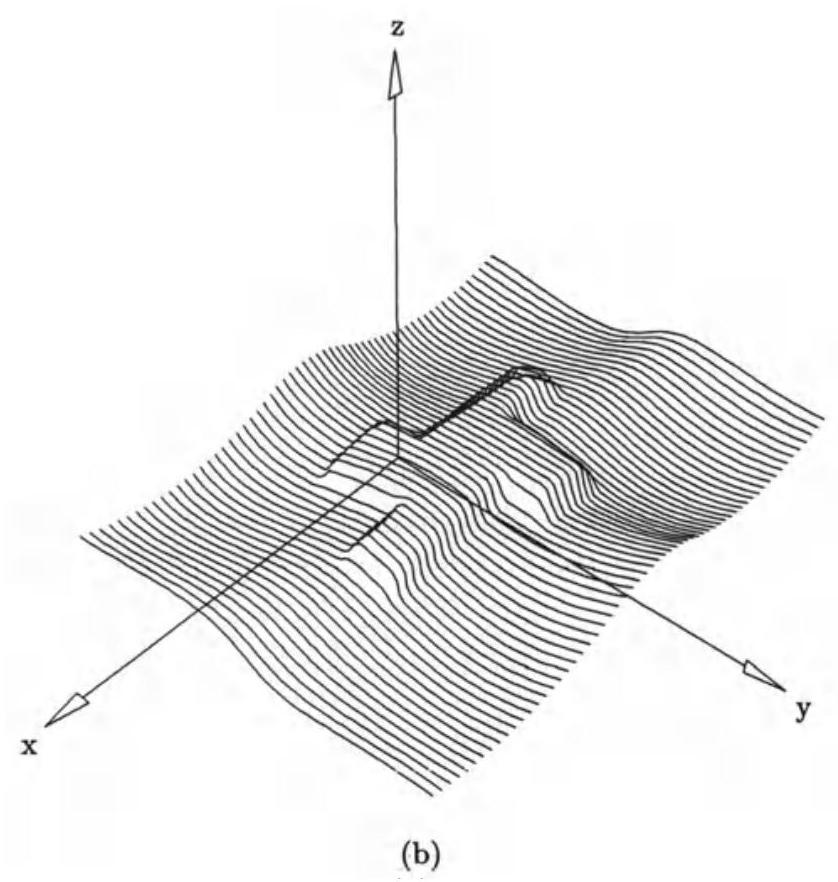
\includegraphics[max width=0.7\textwidth]{images/0193ba0d-ab19-7138-9798-cb281ce60de0_545_365_260_838_882_0.jpg}
\end{center}
\hspace*{3em} 

图11.22.(续)

定义在节点向量上

\[
S = \left\{  {0,0,0,0,\frac{1}{4},\frac{1}{2},\frac{3}{4},1,1,1,1}\right\}
\]

和

\[
T = \left\{  {0,0,0,0,\frac{1}{4},\frac{1}{2},\frac{3}{4},1,1,1,1}\right\}
\]

所有权重均设置为1，除了 \({w}_{3,3}\) ，该值可自由选择。作为另一个例子，如果所需的变形区域表现出圆形对称性，则可以使用旋转的一元B样条基函数。

在任意域上定义变形函数是困难的。图11.22和11.23中的区域变形是使用简单函数创建的。

\[
f\left( {s,t}\right)  = \left\{  \begin{array}{ll} 1 & \text{ if }\left( {u\left( s\right) ,v\left( t\right) }\right)  \in  \mathcal{R} \\  0 & \text{ otherwise } \end{array}\right.  \tag{11.51}
\]

其中

\[
u\left( s\right)  = \left( {{u}_{\beta } - {u}_{\alpha }}\right) s + {u}_{\alpha }\;v\left( t\right)  = \left( {{v}_{\delta } - {v}_{\gamma }}\right) t + {v}_{\gamma }
\]

该变形函数像一个模具冲头，即，每个控制点 \(\left( {u\left( {s}_{i}\right) ,v\left( {t}_{j}\right) }\right)  \in  \mathcal{R}\) 在 \(\mathbf{W}\) 方向上移动了距离 \(d\) 。向量 \(\mathbf{W}\) 可以是每个点的表面法线，或任何其他用户定义的向量。对于图11.22和11.23，使用了光线投射、点在多边形内的例程来确定点在多边形区域内的包含关系。注意在图11.23中，该例程处理自相交的多边形。

\begin{center}
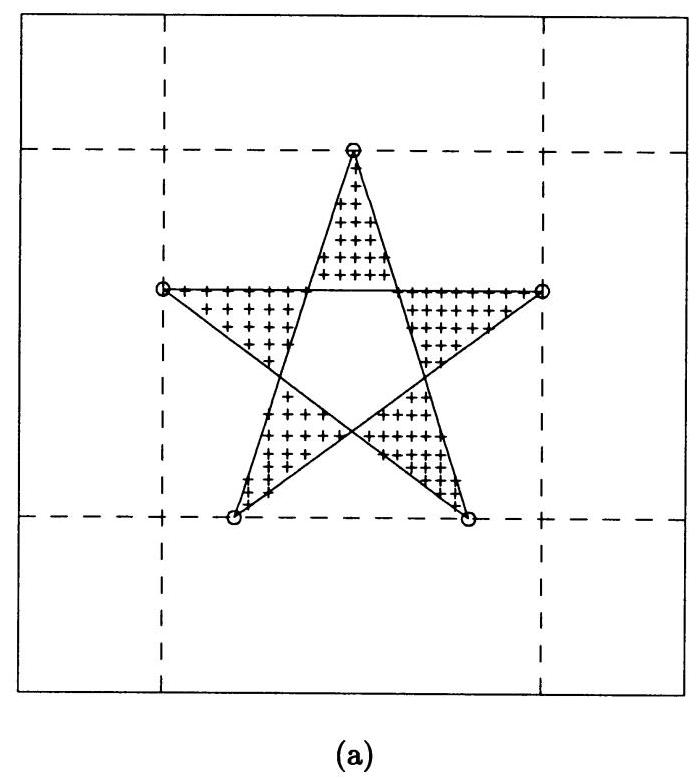
\includegraphics[max width=0.6\textwidth]{images/0193ba0d-ab19-7138-9798-cb281ce60de0_546_423_271_699_779_0.jpg}
\end{center}
\hspace*{3em} 

图11.23. 表面区域变形。(a) 一个具有边界框和局部控制点的区域；(b) 控制点重新定位后的表面变形。

现在我们描述表面曲线变形。假设

\[
\mathbf{C}\left( \lambda \right)  = \left( {u\left( \lambda \right) ,v\left( \lambda \right) }\right)  \tag{11.52}
\]

是位于 \(\mathbf{S}\left( {u,v}\right)\) 参数空间中的一条曲线，而 \(r\) 是沿着每个 \(\lambda\) 在 \(\mathbf{C}\left( \lambda \right)\) 法线方向上测量到 \(\mathbf{C}\left( \lambda \right)\) 两侧的距离。通过重新定位所有那些其参数 \(\left( {u\left( {s}_{i}\right) ,v\left( {t}_{j}\right) }\right)\) 在 \(\mathbf{C}\left( \lambda \right)\) (重力场)距离 \(r\) 范围内的表面控制点 \({\mathbf{P}}_{i,j}\) 来应用表面曲线变形。相关的 \({\mathbf{P}}_{i,j}\) 根据公式移动。

\[
{\widehat{\mathbf{P}}}_{i,j} = {\mathbf{P}}_{i,j} + f\left( {d}_{i,j}\right) d\mathbf{W}\left( {\lambda }_{i,j}\right)  \tag{11.53}
\]

在这里 \({d}_{i,j}\) 是 \(\left( {u\left( {s}_{i}\right) ,v\left( {t}_{j}\right) }\right)\) 到 \(\mathbf{C}\left( \lambda \right)\) 的距离，而 \({\lambda }_{i,j}\) 对应于 \(\left( {u\left( {s}_{i}\right) ,v\left( {t}_{j}\right) }\right)\) 在 \(\mathbf{C}\left( \lambda \right)\) 上的投影。扭曲方向的合理定义是

\[
\mathbf{W}\left( \lambda \right)  = \mathbf{N}\left( {\mathbf{C}\left( \lambda \right) }\right)  \tag{11.54}
\]

在这里 \(\mathbf{N}\left( {u,v}\right)\) 是表面法向量。

\begin{center}
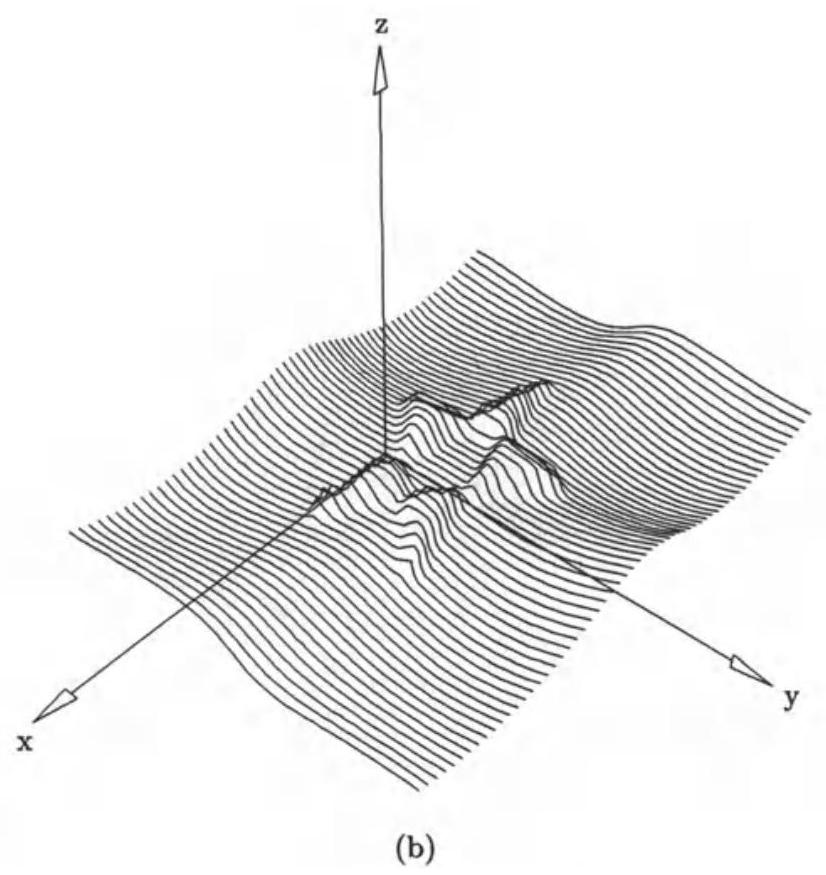
\includegraphics[max width=0.7\textwidth]{images/0193ba0d-ab19-7138-9798-cb281ce60de0_547_351_268_826_875_0.jpg}
\end{center}
\hspace*{3em} 

图 11.23. (续)

再次， \(f\) 的定义可能很微妙。我们使用了这个函数

\[
f\left( {d}_{i,j}\right)  = \left\{  \begin{array}{ll} 1 & \text{ if }{d}_{i,j} \leq  r \\  0 & \text{ otherwise } \end{array}\right.  \tag{11.55}
\]

应用方程 (11.53) 的关键步骤是计算 \({d}_{i,j}\) 。如果 \(\mathbf{C}\left( \lambda \right)\) 是一条折线，这个过程会简化。图 11.24 显示了折线扭曲的一个例子。图 11.24a 描述了由五条折线构成的缩写 NURBS。图 11.24b 显示了控制点的边界框(用 + 标记)，这些控制点位于五个字母的重力场内。最终的折线扭曲表面在图 11.24c 中进行了说明。


\subsection{扁平化}

扁平化操作符允许设计师轻松地将直线段引入曲线和将平面区域引入表面。没有插入多个节点，因此曲线或表面的弯曲部分与平坦部分之间的过渡具有原始几何形状固有的平滑性。

首先考虑曲线扁平化，如图 11.25 和 11.26 所示；给定一条曲线 \(\mathbf{C}\left( u\right)\) 和一条线 \(\mathbf{L}\) 。曲线扁平化由三个步骤组成:

\begin{center}
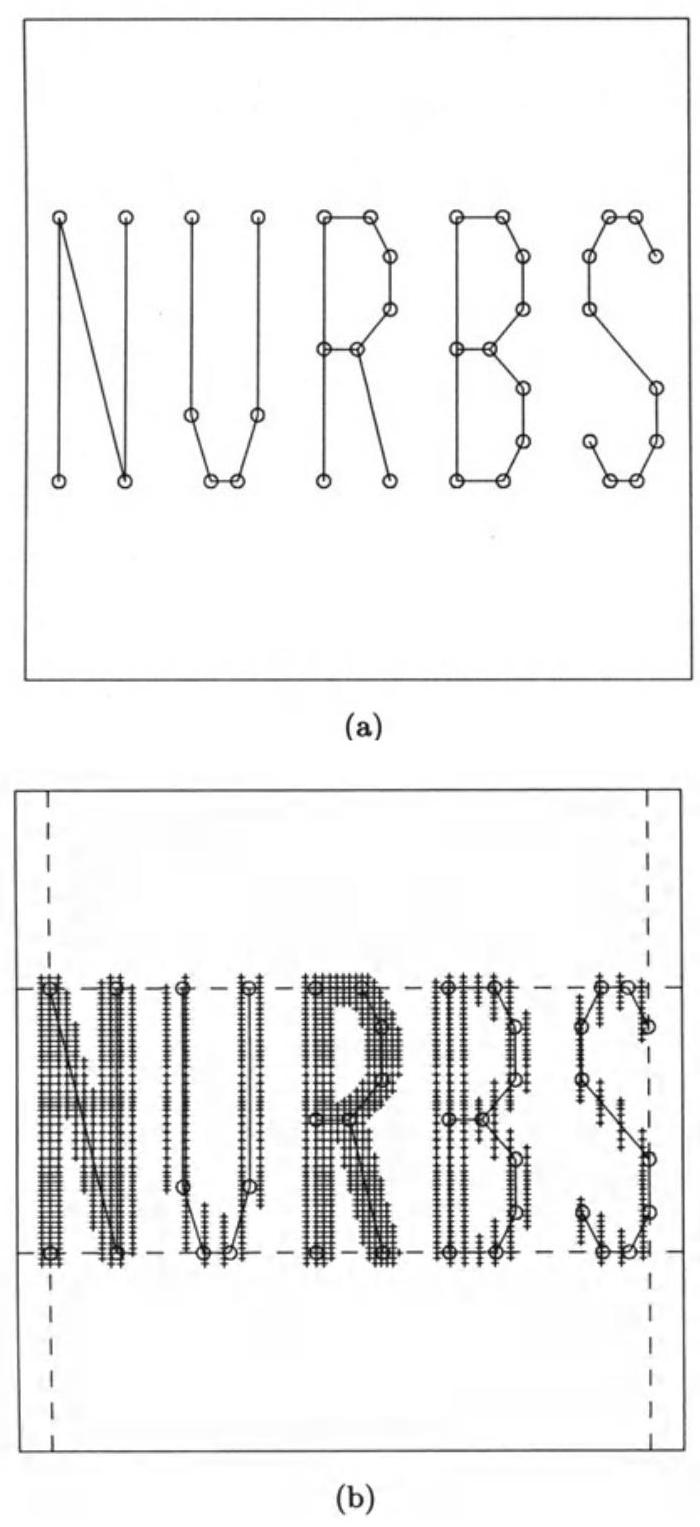
\includegraphics[max width=0.6\textwidth]{images/0193ba0d-ab19-7138-9798-cb281ce60de0_548_423_269_700_1527_0.jpg}
\end{center}
\hspace*{3em} 

图 11.24. 表面折线扭曲。 (a) 表示缩写 NURBS 的折线； (b) 局部于折线重力场的控制点； (c) 控制点重新定位后的表面折线扭曲。

1. 精炼曲线的节点以获得更多控制点；

2. 将一些指定的控制点 \({\mathbf{P}}_{i}\) 投影到该直线上；用 \({\widehat{\mathbf{P}}}_{i}\) 表示 \({\mathbf{P}}_{i}\) 的投影，将 \({\mathbf{P}}_{i}\) 替换为 \({\widehat{\mathbf{P}}}_{i}\) ；

3. 移除不必要的节点。

\begin{center}
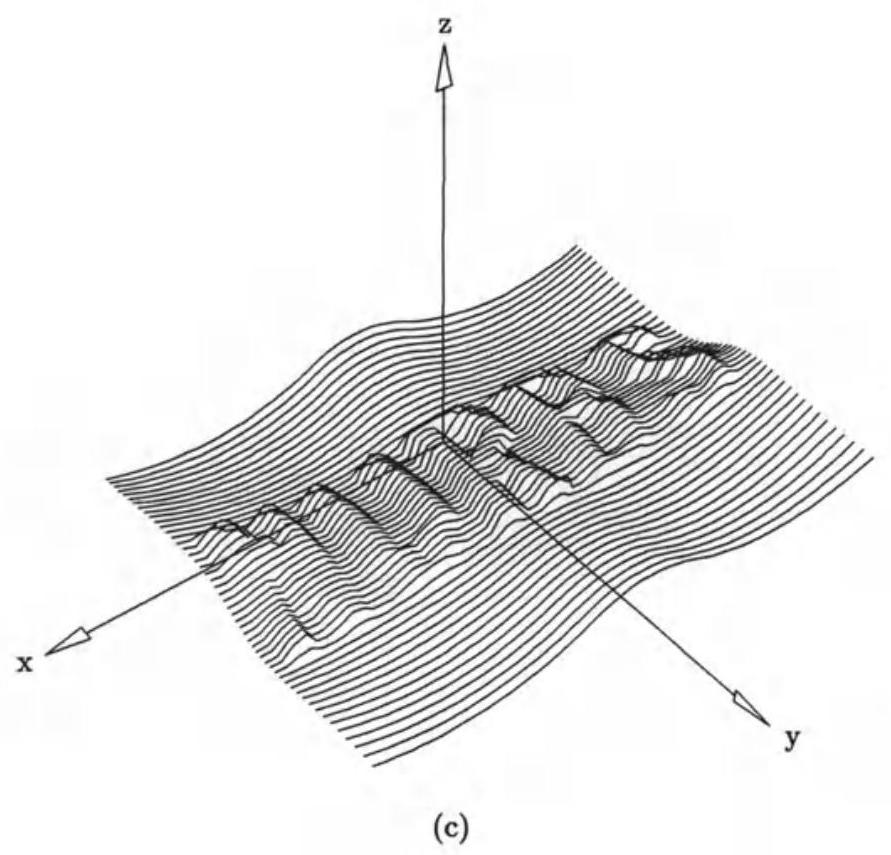
\includegraphics[max width=0.8\textwidth]{images/0193ba0d-ab19-7138-9798-cb281ce60de0_549_339_273_891_855_0.jpg}
\end{center}
\hspace*{3em} 

图 11.24. (续。)

除了 \(\mathbf{L}\) 和 \(\mathbf{C}\left( u\right)\) ，以下项目可以由设计者指定或由系统默认(图 11.25a):

\begin{itemize}
\item 一个向量 \(\mathbf{W}\) ，定义投影线，即 \({\widehat{\mathbf{P}}}_{i} = {\mathbf{P}}_{i} + \alpha \mathbf{W}(\alpha\) 可以是负值或正值；该向量可以默认与 \(\mathbf{L}\) 垂直；
\end{itemize}

\begin{itemize}
\item 参数 \({u}_{s}\) 和 \({u}_{e}\) :只有当控制点 \({\mathbf{P}}_{i}\) 局部于区间 \(\left\lbrack  {{u}_{s},{u}_{e}}\right\rbrack\) 时，才会进行投影，即 \(i = s,\ldots ,e - p - 1\) ；
\end{itemize}

\begin{itemize}
\item 线 \(\mathbf{L}\) 上的两个点 \({\mathbf{Q}}_{1}\) 和 \({\mathbf{Q}}_{2}\) ；只有当控制点 \({\mathbf{P}}_{i}\) 的投影 \({\widehat{\mathbf{P}}}_{i}\) 位于线段 \({\mathbf{Q}}_{1}{\mathbf{Q}}_{2}\) 内时，才会用其投影 \({\widehat{\mathbf{P}}}_{i}\) 替换控制点 \({\mathbf{P}}_{i}\) 。
\end{itemize}

请注意，最后两个项目是规则，分别指示要投影哪些 \({\mathbf{P}}_{i}\) 和接受哪些 \({\widehat{\mathbf{P}}}_{i}\) 。对于图 11.25a 中所示的情况，将 \({\mathbf{Q}}_{1} = \mathbf{C}\left( {u}_{s}\right)\) 和 \({\mathbf{Q}}_{2} = \mathbf{C}\left( {u}_{e}\right)\) 设置为 \(\mathbf{L}\) 与 \(\mathbf{C}\left( u\right)\) 相交的点是一个合理的系统默认值。如果曲线是 \({xy}\) 平面并与 \(\mathbf{L}\) 相交，如图 11.25a 所示，另一个直观的规则是仅投影位于 \(\mathbf{L}\) 一侧的那些 \({\mathbf{P}}_{i}\) ，如图 11.25b 所示。如果仅投影与 \(\left\lbrack  {{u}_{s},{u}_{e}}\right\rbrack\) 相关的控制点，当 \(\mathbf{L}\) 与曲线相交时，可能会出现意外结果(图 11.25c)。如果曲线不与 \(\mathbf{L}\) 相交，则投影所有与 \(\left\lbrack  {{u}_{s},{u}_{e}}\right\rbrack\) 相关的控制点会使线段 \(\left\lbrack  {\mathbf{C}\left( {u}_{s}\right) ,\mathbf{C}\left( {u}_{e}\right) }\right\rbrack\) 平坦化，而曲线的其余部分不受影响。这在图 11.26a 和 11.26b 中得到了说明。

最后，我们提醒注意，只有当投影结果至少为 \(p + 1\) 个连续点时，才能获得平坦的线段， \({\widehat{\mathbf{P}}}_{i}\) ，其中 \(p\) 是曲线的度数。如果

\begin{center}
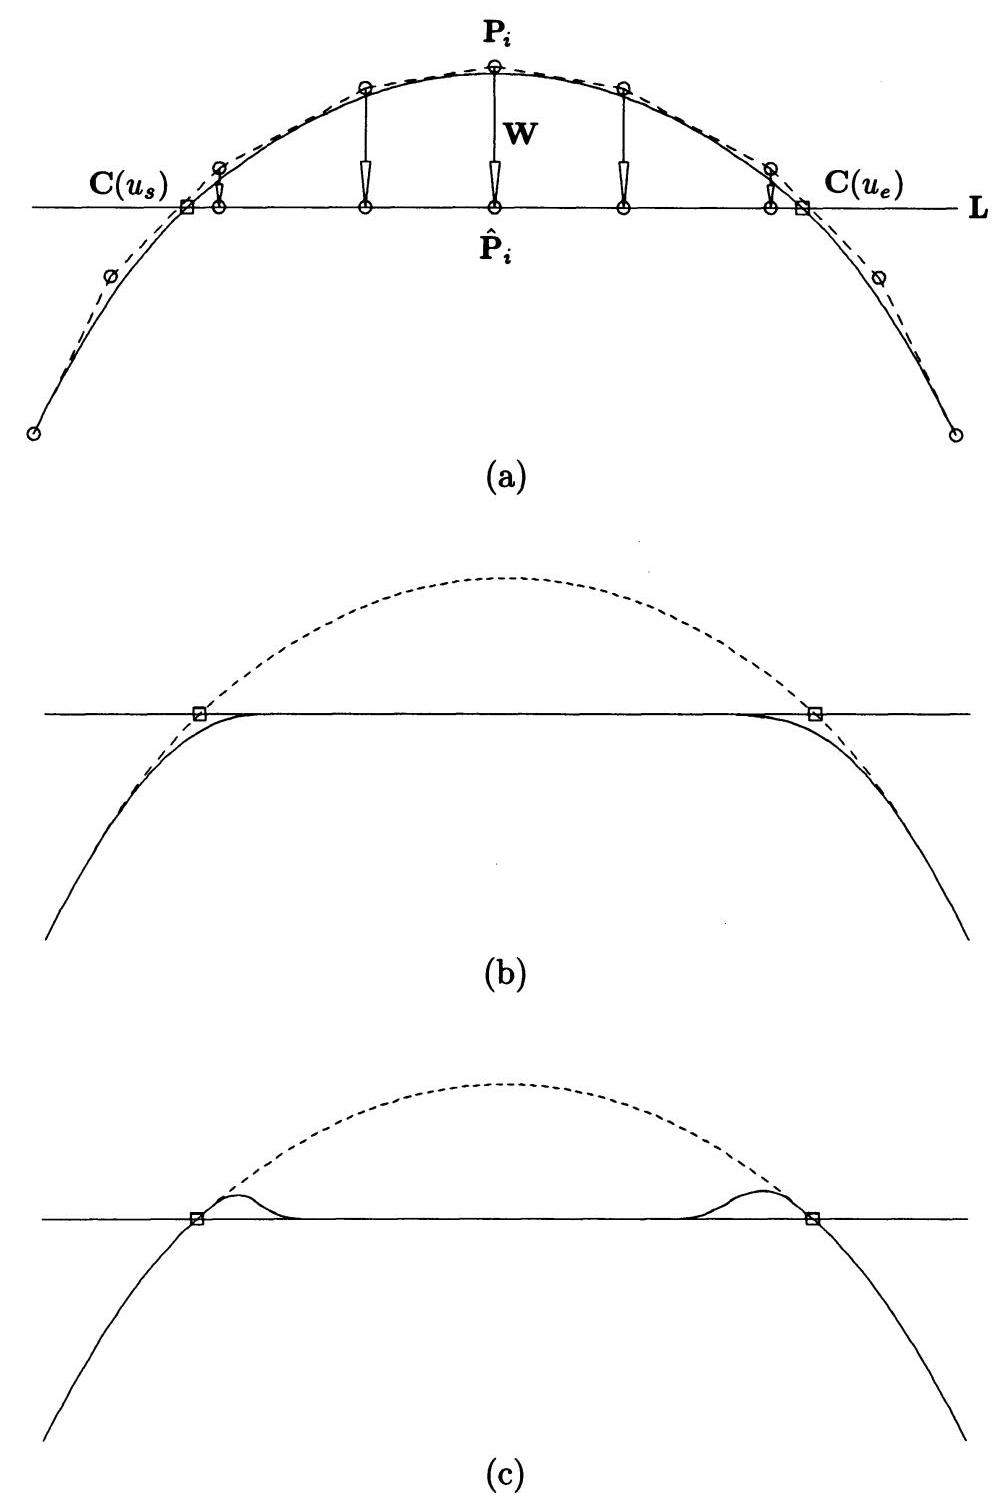
\includegraphics[max width=0.9\textwidth]{images/0193ba0d-ab19-7138-9798-cb281ce60de0_550_264_259_1002_1509_0.jpg}
\end{center}
\hspace*{3em} 

图 11.25. 曲线平坦化。(a) 原始曲线，其跨度为 \(\left\lbrack  {\mathbf{C}\left( {u}_{s}\right) ,\mathbf{C}\left( {u}_{e}\right) }\right\rbrack\) ，将在 \(\mathbf{W}\) 的方向上平坦化，直到与曲线相交的线 \(\mathbf{L}\) ；(b) 通过投影位于 \(\mathbf{L}\) 一侧的所有控制点获得的平坦曲线；(c) 通过投影与跨度 \(\left\lbrack  {{u}_{s},{u}_{e}}\right\rbrack\) 相关的控制点获得的平坦曲线。

如果未能满足该条件，则需要更多的节点细化。如果指定了 \({u}_{s}\) 和 \({u}_{e}\) ，则仅在区间 \(\left\lbrack  {{u}_{i},{u}_{j}}\right\rbrack\) 内需要细化，其中 \({u}_{i}\) 是满足 \({u}_{i} < {u}_{s}\) 的最大节点，而 \({u}_{j}\) 是满足 \({u}_{e} < {u}_{j}\) 的最小节点。

\begin{center}
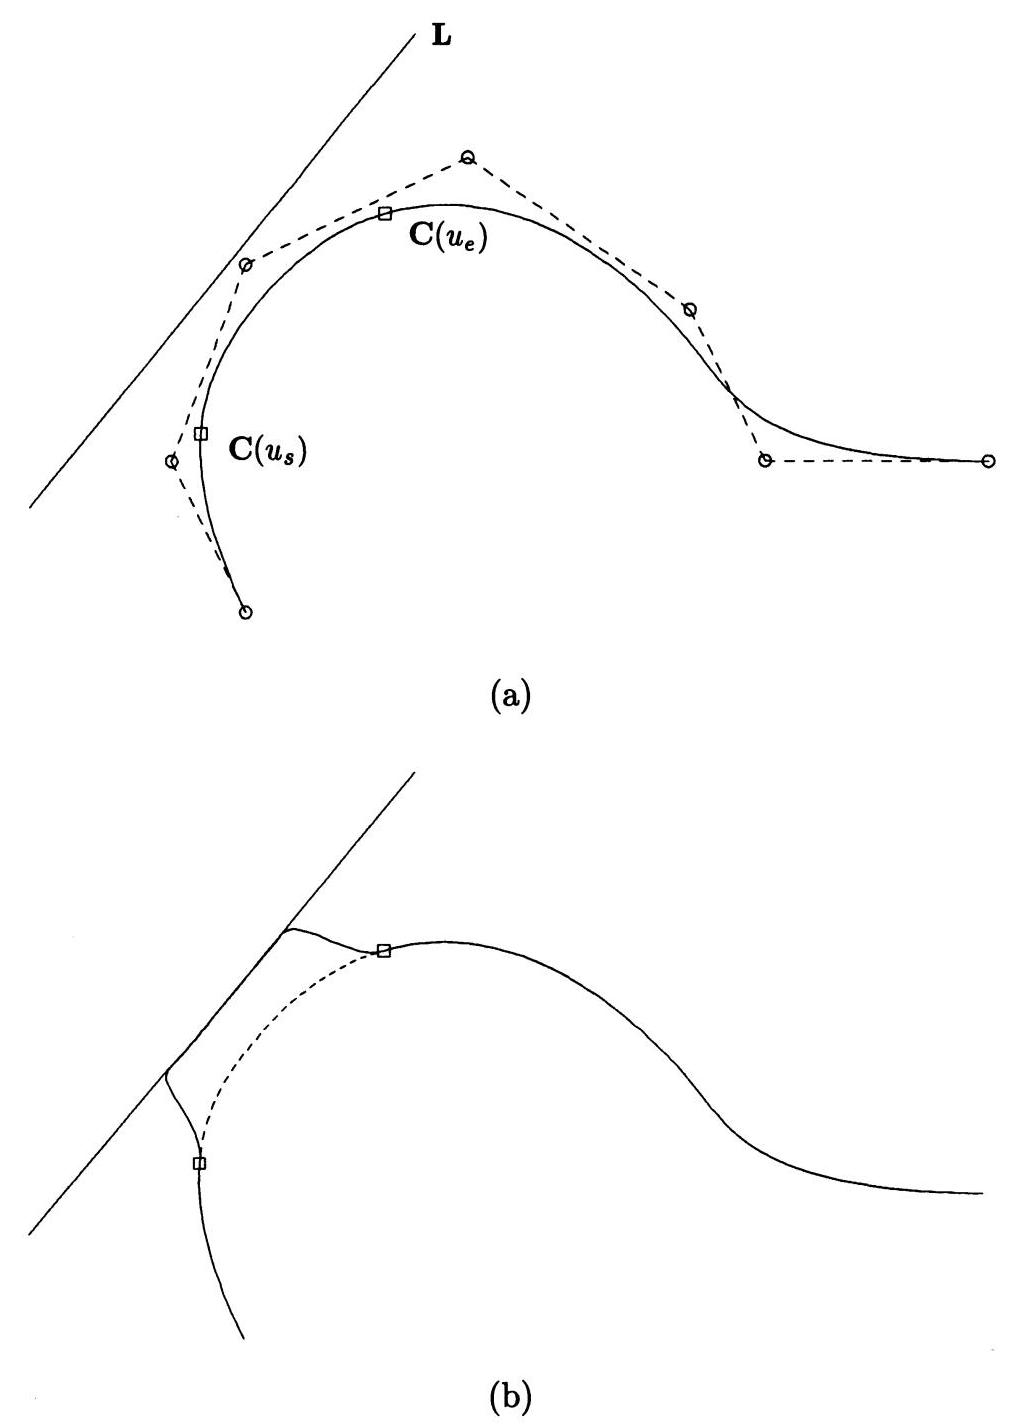
\includegraphics[max width=0.9\textwidth]{images/0193ba0d-ab19-7138-9798-cb281ce60de0_551_259_273_1010_1428_0.jpg}
\end{center}
\hspace*{3em} 

图 11.26. 曲线扁平化。 (a) 原始曲线，其跨度为 \(\left\lbrack  {\mathbf{C}\left( {u}_{s}\right) ,\mathbf{C}\left( {u}_{e}\right) }\right\rbrack\) ，在与不交叉曲线的直线 \(\mathbf{L}\) 垂直的方向上进行扁平化；(b) 通过投影控制点获得的扁平化曲线，控制点局部于跨度 \(\left\lbrack  {{u}_{s},{u}_{e}}\right\rbrack\) 。

通过将控制点 \({\mathbf{P}}_{i,j}\) 投影到平面 \(\pi\) 上来扁平化一个表面区域。 \({\mathbf{P}}_{i,j}\) 被它们的投影 \({\widehat{\mathbf{P}}}_{i,j}\) 替代。除了 \(\pi\) ，还可以指定(或默认)以下内容:

\begin{itemize}
\item 一个向量 \(\mathbf{W}\) 定义投影线，即 \({\widehat{\mathbf{P}}}_{i,j} = {\mathbf{P}}_{i,j} + \alpha \mathbf{W}(\alpha\) 可以是负值或正值；该向量可以默认设置为与 \(\pi\) 垂直；
\end{itemize}

\begin{itemize}
\item 一个区域 \({\mathcal{R}}_{uv}\) ，在 \({uv}\) 空间中由边界曲线定义，只有当其影响局限于区域 \({\mathcal{R}}_{uv}\) 时， \({\mathbf{C}}_{uv}\left( w\right)  = \left( {u\left( w\right) ,v\left( w\right) }\right) ;{\mathbf{P}}_{i,j}\) 才会被投影。如果 \(\left\lbrack  {{u}_{\alpha },{u}_{\beta }}\right\rbrack   \times  \left\lbrack  {{v}_{\gamma },{v}_{\delta }}\right\rbrack\) 是包含 \({\mathcal{R}}_{uv}\) 的最小最大矩形，则应对区间 \(\left\lbrack  {{u}_{i},{u}_{j}}\right\rbrack\) 和 \(\left\lbrack  {{v}_{k},{v}_{\ell }}\right\rbrack\) 应用节点细化，其中 \({u}_{i}\) 和 \({v}_{k}\) 是满足 \({u}_{i} < {u}_{\alpha }\) 和 \({v}_{k} < {v}_{\gamma }\) 的最大节点，而 \({u}_{j}\) 和 \({v}_{\ell }\) 是满足 \({u}_{\beta } < {u}_{j}\) 和 \({v}_{\delta } < {v}_{\ell }\) 的最小节点。
\end{itemize}

\begin{itemize}
\item 一个区域， \({\mathcal{R}}_{\pi }\) ，在平面上 \(\pi\) ，由边界曲线 \({\mathbf{C}}_{\pi }\left( w\right)\) 定义；控制点 \({\mathbf{P}}_{i,j}\) 仅在 \({\widehat{\mathbf{P}}}_{i,j}\) 位于区域 \({\mathcal{R}}_{\pi }\) 内时被其投影 \({\widehat{\mathbf{P}}}_{i,j}\) 替代。
\end{itemize}

最常见的是， \({\mathbf{C}}_{uv}\left( w\right)\) 和 \({\mathbf{C}}_{\pi }\left( w\right)\) 是简单曲线，例如多边形或圆，对于这些曲线，确定点是否包含在相应区域内是简单且高效的。如果平面 \(\pi\) 与表面相交，则设计者可能希望指定仅在 \(\pi\) 一侧的那些 \({\mathbf{P}}_{i,j}\) 被投影，而不是要求一个区域 \({\mathcal{R}}_{uv}\) 。Cobb [Cobb84]建议使用额外的平面来限制要投影的控制网区域。最后，投影必须产生至少 \(\left( {p + 1}\right)  \times  \left( {q + 1}\right) {\widehat{\mathbf{P}}}_{i,j}\) 的连接网格，以便在表面上获得一个平坦区域。图11.27a和11.27b展示了表面展平的一个例子。


\subsection{弯曲}

几位作者研究了曲线的圆形弯曲和表面的圆柱形弯曲，例如，参见文献[Barr83; Four83; Cobb84]。这些作者基于三角学发展了将点映射到圆上的方程。在这些映射下，直线段映射到一个圆上，而一般曲线段则以圆形方式弯曲。Cobb [Cobb84]将这种技术与节点细化相结合，应用于控制点的映射，从而弯曲B样条曲线和表面。

我们采取一种更一般的几何方法来进行弯曲。类似于其他形状操作，弯曲分为三个步骤:

1. 细化要弯曲的曲线或表面区域；

2. 通过重新定位控制点来弯曲区域；

3. 移除不必要的节点。

只有步骤 2 需要详细说明。首先考虑曲线(见图 11.28)。我们将曲线 \(\mathbf{C}\left( u\right)\) 在 \(\mathbf{C}\left( {u}_{s}\right)\) 和 \(\mathbf{C}\left( {u}_{e}\right)\) 之间的区域围绕弯曲曲线 \(\mathbf{B}\left( w\right)\) 进行弯曲，通过将相关控制点 \({\mathbf{P}}_{i}\) 映射到 \(\mathbf{B}\left( w\right)\) 的“方向”。假设 \({u}_{s}\) 和 \({u}_{e}\) 是节点，仅映射 \({\mathbf{P}}_{s},\ldots ,{\mathbf{P}}_{e - p - 1}\) 。将 \({\mathbf{P}}_{i}\) 的图像表示为 \({\widehat{\mathbf{P}}}_{i}\) 。我们需要一个额外的点 \(\mathbf{O}\) ，称为弯曲中心。点 \({\mathbf{R}}_{i}\) 是通过将每个线段 \({\mathbf{{OP}}}_{i}\) 与 \(\mathbf{B}\left( w\right)\) 相交得到的。最后，固定一个交叉比 \(\lambda\) ，每个 \({\widehat{\mathbf{P}}}_{i}\) 的位置由 \(\lambda ,\mathbf{O},{\mathbf{R}}_{i}\) 和 \({\mathbf{P}}_{i}\) 确定，如下所示。类似于公式 (11.22)，我们有

\[
{\mathbf{R}}_{i} = \left( {1 - {s}_{i}}\right) \mathbf{O} + {s}_{i}{\mathbf{P}}_{i}
\]

548 形状修改工具

\[
{\widehat{\mathbf{P}}}_{i} = \left( {1 - {t}_{i}}\right) \mathbf{O} + {t}_{i}{\mathbf{P}}_{i} \tag{11.56}
\]

\begin{center}
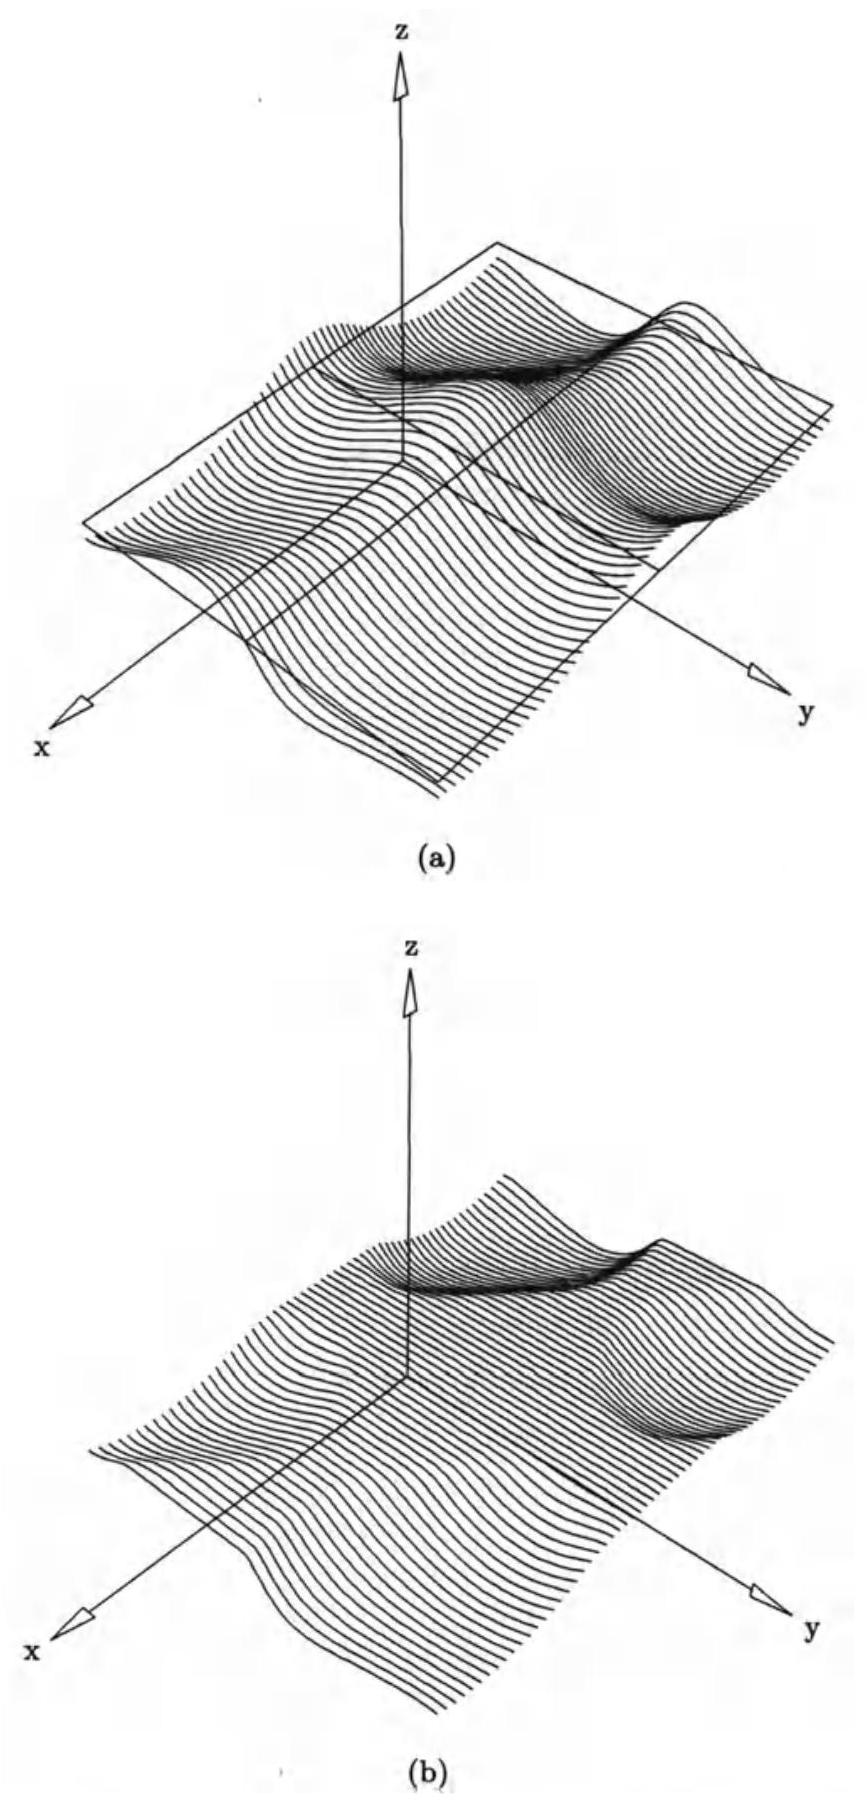
\includegraphics[max width=0.7\textwidth]{images/0193ba0d-ab19-7138-9798-cb281ce60de0_553_346_271_867_1800_0.jpg}
\end{center}
\hspace*{3em} 

图 11.27. 表面展平。(a)一个表面和一个平面；(b)通过投影所有位于平面一侧的控制点获得的展平表面。

\begin{center}
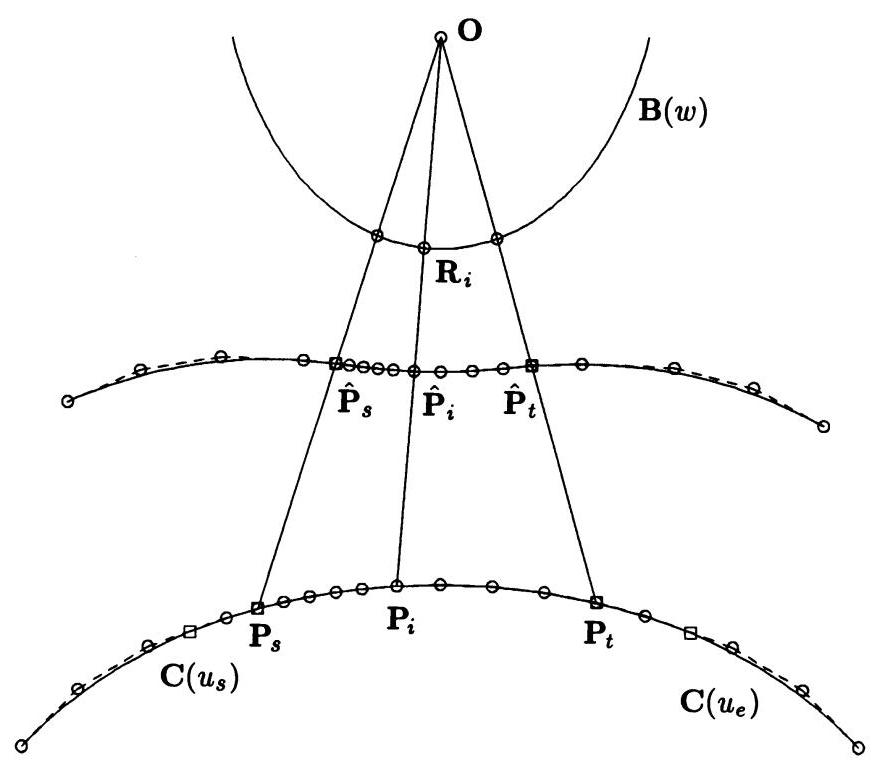
\includegraphics[max width=0.8\textwidth]{images/0193ba0d-ab19-7138-9798-cb281ce60de0_554_330_272_875_765_0.jpg}
\end{center}
\hspace*{3em} 

图 11.28. 曲线弯曲。

由此可得

\[
{s}_{i} = \frac{{\mathbf{{OR}}}_{i}}{{\mathbf{{OP}}}_{i}} \tag{11.57}
\]

最后

\[
\lambda  = \frac{{t}_{i}\left( {1 - {s}_{i}}\right) }{{s}_{i}\left( {1 - {t}_{i}}\right) }
\]

产生

\[
{t}_{i} = \frac{\lambda {s}_{i}}{1 + \left( {\lambda  - 1}\right) {s}_{i}} \tag{11.58}
\]

将 \({t}_{i}\) 代入公式 (11.56) 产生 \({\widehat{\mathbf{P}}}_{i}\) 。

总结来说， \({u}_{s},{u}_{e},\mathbf{B}\left( w\right) ,\mathbf{O}\) 和 \(\lambda\) 被给出，弯曲算法依次计算: \({\mathbf{R}}_{i}\) (线/曲线交点)、 \({s}_{i},{t}_{i}\) 和 \({\widehat{\mathbf{P}}}_{i}\) 。交叉比 \(\lambda\) 可以在 \(- \infty\) 到 \(\infty\) 的范围内进行交互式修改。注意 \(\lambda  = 1\) 意味着 \({t}_{i} = {s}_{i}\) ，因此 \({\widehat{\mathbf{P}}}_{i} = {\mathbf{R}}_{i}\) ；即 \(\lambda  = 1\) 将所有 \({\mathbf{P}}_{i}\) 映射到 \(\mathbf{B}\left( w\right)\) ，因此 \(\mathbf{C}\left( u\right)\) 在 \(\mathbf{C}\left( {u}_{s}\right)\) 和 \(\mathbf{C}\left( {u}_{e}\right)\) 之间的区域假设了 \(\mathbf{B}\left( w\right)\) 的(近似)形状。对于 \(\lambda  = 0\) ，所有 \({\widehat{\mathbf{P}}}_{i} = \mathbf{O}\) ；以及 \({\widehat{\mathbf{P}}}_{i} \rightarrow  {\mathbf{P}}_{i}\) 作为 \(\lambda  \rightarrow  \infty\) 。

设 \(t = e - p - 1\) 。在计算 \({\widehat{\mathbf{P}}}_{s},\ldots ,{\widehat{\mathbf{P}}}_{t}\) 后，控制点 \({\mathbf{P}}_{0},\ldots ,{\mathbf{P}}_{s - 1}\) 和 \({\mathbf{P}}_{t + 1},\ldots ,{\mathbf{P}}_{n}\) 必须旋转并平移到位置，以实现 \(\left\lbrack  {{u}_{\min },{u}_{s}}\right\rbrack\) 和 \(\left\lbrack  {{u}_{e},{u}_{\max }}\right\rbrack\) 上未改变的曲线段与 \(\left\lbrack  {{u}_{s},{u}_{e}}\right\rbrack\) 上的弯曲段之间的自然过渡。设 \(\theta\) 表示弯曲映射旋转向量 \({\mathbf{P}}_{t} - {\mathbf{P}}_{t - 1}\) 的角度。新的 \({\widehat{\mathbf{P}}}_{t + 1},\ldots ,{\widehat{\mathbf{P}}}_{n}\) 通过围绕点 \({\mathbf{P}}_{t}\) 旋转 \({\mathbf{P}}_{t + 1},\ldots ,{\mathbf{P}}_{n}\) 一个角度 \(\theta\) ，然后通过向量 \({\widehat{\mathbf{P}}}_{t} - {\mathbf{P}}_{t}\) 进行平移而获得。类似的旋转(由 \(\left. {{\mathbf{P}}_{s + 1} - {\mathbf{P}}_{s}}\right)\) 的旋转定义)和平移必须应用于 \({\mathbf{P}}_{0},\ldots ,{\mathbf{P}}_{s - 1}\) 。

图 11.29-11.31 显示了圆形和抛物线弯曲的示例。在图 11.29 中，变化 \(\lambda\) 的效果得到了说明。弯曲区域关于通过弯曲中心 \(\mathbf{O}\) 的线 \(\mathbf{L}\) 是对称的，并且与 \(\mathbf{C}\left( u\right)\) 垂直。注意，当 \(\lambda\) 接近 1 时，弯曲区域逐渐呈现出圆形的形状。图 11.30 显示了将中心 O 放置在圆内的效果。 \({\mathbf{O}}_{1}\) 是圆心， \({\mathbf{O}}_{2}\) 位于线 \(\mathbf{L}\) 上，而 \({\mathbf{O}}_{3}\) 是一个任意点。图 11.31 说明了使用抛物线弯曲曲线来消除曲线中的两个不必要的拐点。

最后，我们指出，为了实现额外的形状控制，交叉比可以是一个函数 \(\lambda \left( u\right)\) ，定义在 \(u \in  \left\lbrack  {{u}_{s},{u}_{e}}\right\rbrack\) 上。然后计算 \({\mathbf{P}}_{i},{\lambda }_{i} = \lambda \left( {t}_{i}\right)\) ，其中 \({t}_{i}\) 是第 \(i\) 个节点(与方程 [11.58] 的 \({t}_{i}\) 无关)。

现在我们转向表面弯曲。曲线弯曲技术向表面的自然扩展产生了非常一般和强大的表面修改能力。我们从表面弯曲的一般定义开始，但随后将详细讨论限制在一个简单但有用的特例上。

一个表面 \(\mathbf{S}\left( {u,v}\right)\) 围绕一个弯曲表面 \(\mathbf{B}\left( {s,t}\right)\) 弯曲，朝向一个中心点 \(\mathbf{O}\) 或一个中心曲线 \(\mathbf{O}\left( w\right)\) 。设弯曲区域 \(\mathcal{R}\) 在 \({uv}\) 空间中被最小最大矩形 \(\mathcal{M} = \left\lbrack  {{u}_{\alpha },{u}_{\beta }}\right\rbrack   \times  \left\lbrack  {{v}_{\gamma },{v}_{\delta }}\right\rbrack\) 所限制。在对控制点的子集 \({\mathbf{P}}_{i,j},i = \alpha ,\ldots ,\beta  - p - 1,j = \gamma ,\ldots ,\delta  - q - 1\) 进行节点细化后，其对 \(\mathcal{R}\) 的影响是局部的，映射到新位置 \({\widehat{\mathbf{P}}}_{i,j}\) ，使用交叉比 \(\lambda\) ；也可以使用一个函数 \(\lambda \left( {u,v}\right)\) 。如果使用一个点 \(\mathbf{O}\) ，则通过线段 \({\mathbf{{OP}}}_{i,j}\) 与表面 \(\mathbf{B}\left( {s,t}\right)\) 的交点获得点 \({\mathbf{R}}_{i,j}\) 。如果给定一条曲线 \(\mathbf{O}\left( w\right)\) ，则必须计算参数 \({w}_{i,j}\) ，并通过将 \(\mathbf{O}\left( {w}_{i,j}\right) {\mathbf{P}}_{i,j}\) 与 \(\mathbf{B}\left( {s,t}\right)\) 相交来获得 \({\mathbf{R}}_{i,j}\) 。然后计算 \({\widehat{\mathbf{P}}}_{i,j}\) 。

\[
{s}_{i,j} = \frac{{\mathbf{{OR}}}_{i,j}}{{\mathbf{{OP}}}_{i,j}}\;\text{ or }\;{s}_{i,j} = \frac{\mathbf{O}\left( {w}_{i,j}\right) {\mathbf{R}}_{i,j}}{\mathbf{O}\left( {w}_{i,j}\right) {\mathbf{P}}_{i,j}} \tag{11.59}
\]

\[
{t}_{i,j} = \frac{\lambda {s}_{i,j}}{1 + \left( {\lambda  - 1}\right) {s}_{i,j}} \tag{11.60}
\]

\begin{center}
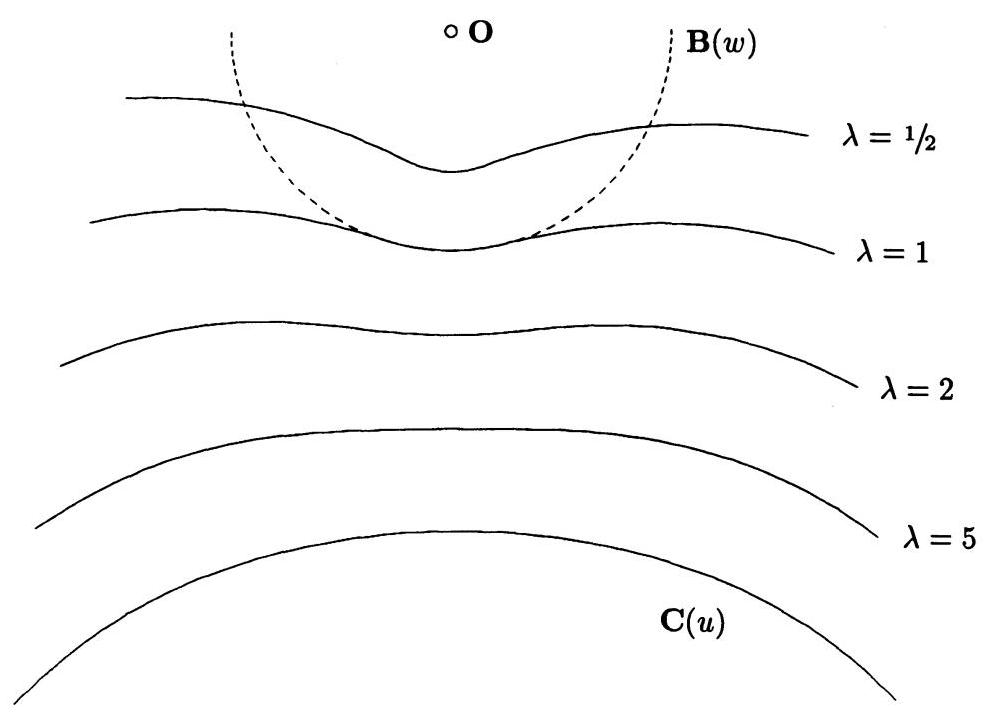
\includegraphics[max width=0.9\textwidth]{images/0193ba0d-ab19-7138-9798-cb281ce60de0_555_273_1311_988_718_0.jpg}
\end{center}
\hspace*{3em} 

图 11.29。使用圆弧作为弯曲曲线的曲线弯曲示例 \(\mathbf{B}\left( w\right)\) ；交叉比为 \(\lambda  = \left\{  {1/2,1,2,5}\right\}\) 。

\begin{center}
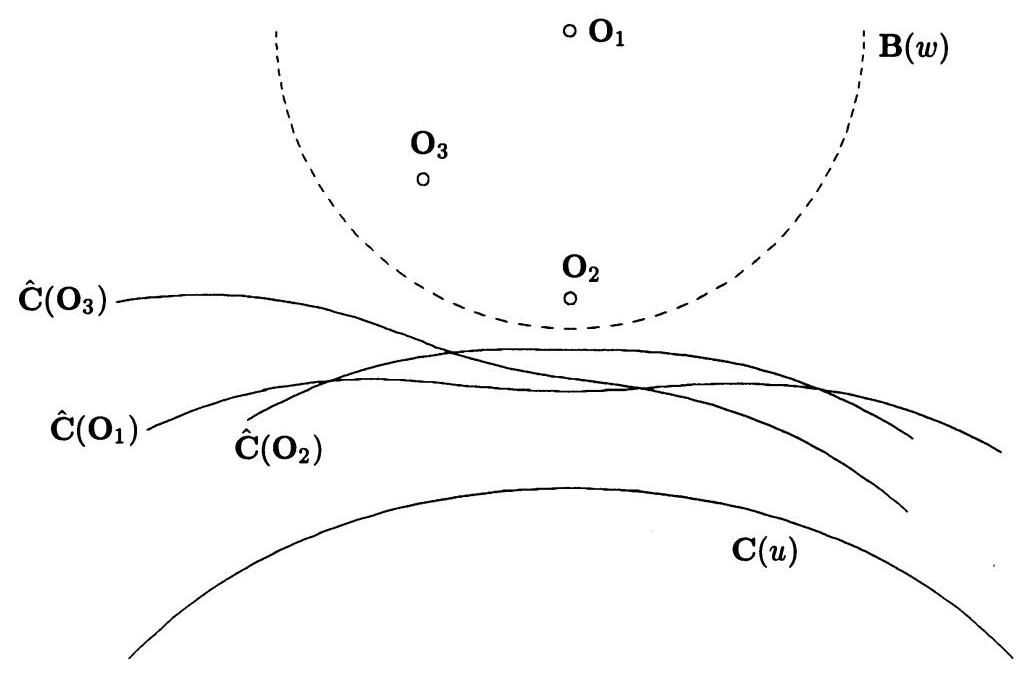
\includegraphics[max width=0.9\textwidth]{images/0193ba0d-ab19-7138-9798-cb281ce60de0_556_256_268_1026_674_0.jpg}
\end{center}
\hspace*{3em} 

图 11.30。通过使用不同的弯曲中心位置获得的曲线弯曲示例。

最后

\[
{\widehat{\mathbf{P}}}_{i,j} = \left( {1 - {t}_{i,j}}\right) \mathbf{O} + {t}_{i,j}{\mathbf{P}}_{i,j}\;\mathrm{{or}}\;{\widehat{\mathbf{P}}}_{i,j} = \left( {1 - {t}_{i,j}}\right) \mathbf{O}\left( {w}_{i,j}\right)  + {t}_{i,j}{\mathbf{P}}_{i,j} \tag{11.61}
\]

随后，未映射的控制点必须旋转和平移到确保弯曲区域平滑自然过渡到未弯曲区域的位置。节点移除作为最后一步应用。例如，通过让 \(\mathbf{B}\left( {s,t}\right)\) 为一个球体，中心为 \(\mathbf{O}\) ，可以获得一个球形弯曲。如果 \(\mathbf{B}\left( {s,t}\right)\) 是一个圆柱体，而 \(\mathbf{O}\left( w\right)\) 是其轴，则会产生一个圆柱形弯曲。

在其完全一般性下，表面弯曲显然是复杂的。 \({\mathbf{R}}_{i,j}\) 的计算需要线/面交点，获得合适的参数 \({w}_{i,j}\) 可能很困难，并且如何旋转和移动未映射的控制点并不明显。我们在此详细说明关于表面等值线全长的通用圆柱形弯曲的特殊情况；即，弯曲区域具有 \(\left\lbrack  {{u}_{\alpha },{u}_{\beta }}\right\rbrack   \times  \left\lbrack  {{v}_{\min },{v}_{\max }}\right\rbrack\) 或 \(\left\lbrack  {{u}_{\min },{u}_{\max }}\right\rbrack   \times  \left\lbrack  {{v}_{\gamma },{v}_{\delta }}\right\rbrack\) 的形式，而 \(\mathbf{B}\left( {s,t}\right)\) 是通过沿着(可能是弯曲的)轴线扫过一个圆而获得的通用圆柱体。

\begin{center}
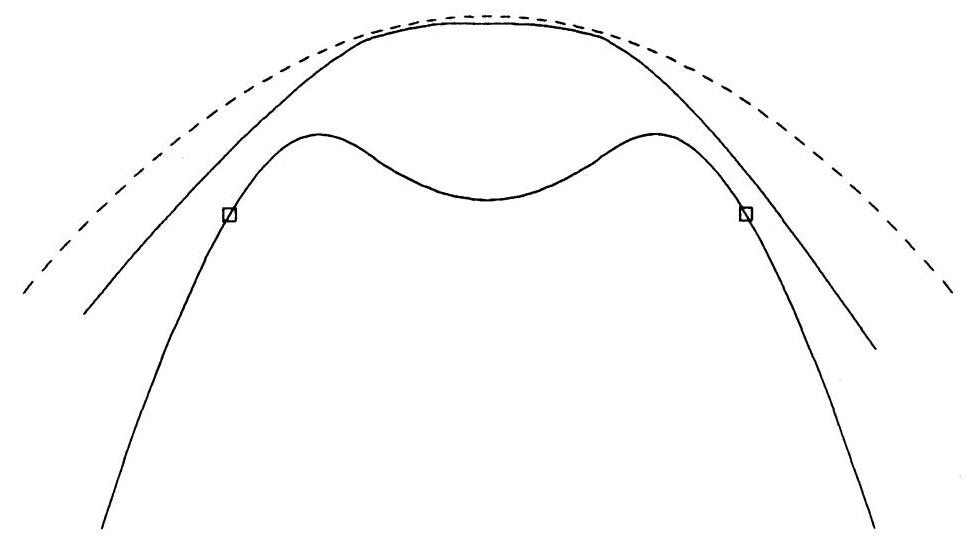
\includegraphics[max width=0.8\textwidth]{images/0193ba0d-ab19-7138-9798-cb281ce60de0_557_282_375_968_542_0.jpg}
\end{center}
\hspace*{3em} 

图 11.31. 用于消除拐点的抛物线弯曲。

\(\mathbf{O}\left( w\right)\) 。我们展示了在固定 \(u = {u}_{c}\) 下关于等值线的弯曲；固定 \(v = {v}_{c}\) 的情况是类似的。假设 \({u}_{c},{u}_{\alpha }\) 和 \({u}_{\beta }\) 满足 \({u}_{\alpha } < {u}_{c} < {u}_{\beta }\) 。令 \({\mathbf{C}}_{{u}_{c}}\left( v\right)\) 表示在 \(\mathbf{S}\left( {u,v}\right)\) 上的等值线，位于 \(u = {u}_{c}\) (见图 11.32)。轴 \(\mathbf{O}\left( w\right)\) 可以通过两种方式定义。它可以被定义为沿着表面法线的 \({\mathbf{C}}_{{u}_{c}}\left( v\right)\) 的偏移，即。

\[
\mathbf{O}\left( v\right)  = {\mathbf{C}}_{{u}_{c}}\left( v\right)  + d\mathbf{N}\left( {{u}_{c},v}\right)  \tag{11.62}
\]

\begin{center}
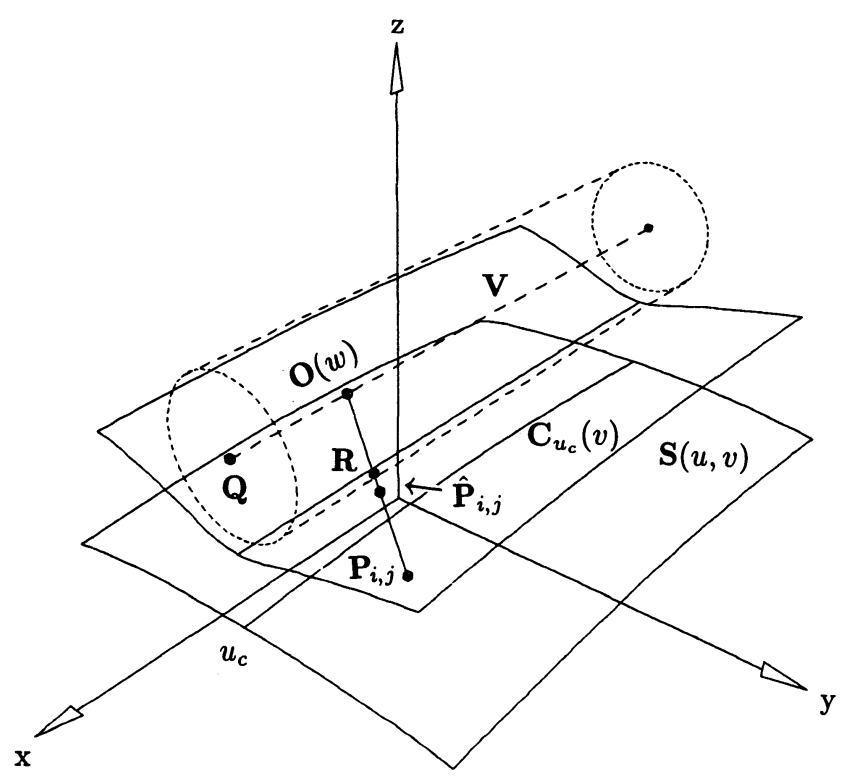
\includegraphics[max width=0.7\textwidth]{images/0193ba0d-ab19-7138-9798-cb281ce60de0_557_344_1304_847_782_0.jpg}
\end{center}
\hspace*{3em} 

图 11.32. 使用圆柱体的表面弯曲。

在这里， \(\mathbf{N}\left( {{u}_{c},v}\right)\) 是位于 \(\left( {{u}_{c},v}\right)\) 的单位长度表面法向量， \(d\) 是一个常量偏移距离。我们注意到，通常情况下， \(\mathbf{O}\left( v\right)\) 的形状可能与 \({\mathbf{C}}_{{u}_{c}}\left( v\right)\) 的形状截然不同，并且 \(\mathbf{O}\left( v\right)\) 不能精确表示为 NURBS 曲线(例如，见 [Till84; Coqu87b; Hosc88])。然而，我们在这里假设 \(\mathbf{O}\left( v\right)\) 行为良好，并且在形状上与 \({\mathbf{C}}_{{u}_{c}}\left( v\right)\) 相似；对于表面弯曲，这是一个合理的假设。此外，我们只需要计算 \(\mathbf{O}\left( v\right)\) 上的选定点(使用公式 [11.62])；我们不需要 \(\mathbf{O}\left( v\right)\) 的显式 NURBS 表示。最后，我们注意到在这种情况下，参数 \(w\) 对应于 \(v\) 。

定义 \(\mathbf{O}\left( w\right)\) 的第二种方法是让它成为位于 \({\mathbf{C}}_{{u}_{c}}\left( v\right)\) 定义的平面中的一条直线。在这种情况下， \(w\) 并不对应于 \(v\) 。通过计算一个最小二乘平面(由 \({\mathbf{C}}_{{u}_{c}}\left( v\right)\) 的控制点定义)，该方法甚至可以用于非平面 \({\mathbf{C}}_{{u}_{c}}\left( v\right)\) 。

通过对 \(m + 1\) 控制点的行应用曲线弯曲方法来弯曲 \(\mathbf{S}\left( {u,v}\right)\) ；即，对于 \(j = 0,\ldots ,m\) ，执行以下操作:

1. 对于 \(i = s,\ldots ,e - p - 1\) :

1a. 计算 \({w}_{i,j}\) ，使得 \(\mathbf{O}\left( {w}_{i,j}\right)\) 是 \(\mathbf{O}\left( w\right)\) 上离 \({\mathbf{P}}_{i,j}\) 最近的点；如果

\(\mathbf{O}\left( w\right)  = \mathbf{Q} + w\mathbf{V}\) 是一条直线，则 \({w}_{i,j}\) 由公式给出

\[
{w}_{i,j} = \frac{\mathbf{V} \cdot  \left( {{\mathbf{P}}_{i,j} - \mathbf{Q}}\right) }{{\left| \mathbf{V}\right| }^{2}} \tag{11.63}
\]

如果 \(\mathbf{O}\left( w\right)\) 是 \({\mathbf{C}}_{{u}_{c}}\left( v\right)\) 的偏移量，则可以使用第 (6.1) 节的点到曲线投影技术；第 \(j\) 个 \(v\) 节点 \({t}_{j}\) 是牛顿迭代的良好起始点；

1b. 然后设置

\[
{\mathbf{R}}_{i,j} = \mathbf{O}\left( {w}_{i,j}\right)  + r\frac{{\mathbf{P}}_{i,j} - \mathbf{O}\left( {w}_{i,j}\right) }{\left| {\mathbf{P}}_{i,j} - \mathbf{O}\left( {w}_{i,j}\right) \right| } \tag{11.64}
\]

其中 \(r\) 是一般圆柱体 \(\mathbf{B}\left( {s,t}\right)\) 的半径；

1c. 使用公式 (11.59)-(11.61) 计算 \({\widehat{\mathbf{P}}}_{i,j}\) ；

2. 通过类似于曲线弯曲的过程，将 \({\mathbf{P}}_{0,j},\ldots ,{\mathbf{P}}_{s - 1,j}\) 和 \({\mathbf{P}}_{e - p,j},\ldots ,{\mathbf{P}}_{n,j}\) 旋转并平移到新位置。

图 11.33 和 11.34 显示了圆柱面弯曲的示例。在图 11.33 中，平面表面使用 \(\lambda  = \left\{  {1/2,3/2, - 3}\right\}\) 进行弯曲。注意，正的 \(\lambda\) 会将表面弯曲向圆柱内，而负的则会将其弯曲远离圆柱。图 11.34 显示了使用沿等参数曲线 \({\mathbf{C}}_{{u}_{c}}\left( v\right)\) 接触表面的圆柱对同一平面表面的圆柱弯曲。同样， \(\lambda\) 的符号允许表面向两个方向弯曲。重要的是要注意，尽管表面是平面的，但它的度数不是 \(\left( {1 \times  1}\right)\) ；图 11.34 中的表面具有度数 \(\left( {3 \times  2}\right)\) 。一般来说，表面必须至少具有度数 \(\left( {2 \times  2}\right)\) ，以避免在控制点重新定位后出现不连续性。554 形状修改工具

\begin{center}
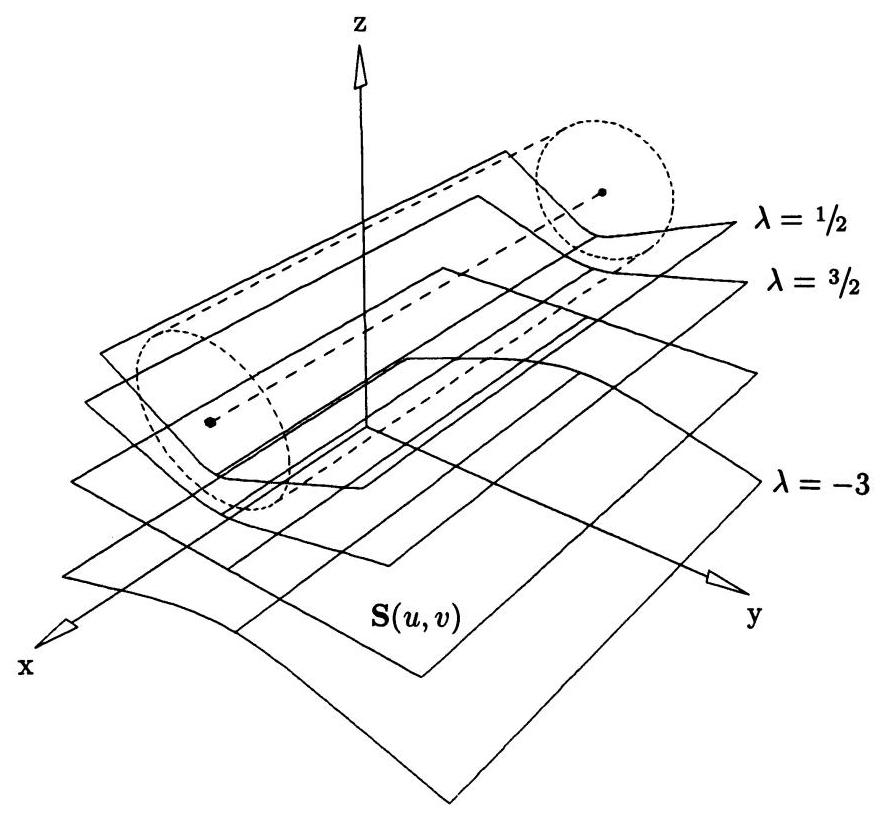
\includegraphics[max width=0.8\textwidth]{images/0193ba0d-ab19-7138-9798-cb281ce60de0_559_325_250_888_813_0.jpg}
\end{center}
\hspace*{3em} 

图 11.33. 使用不接触圆柱的表面弯曲示例， \(\lambda  = \left\{  {1/2,3/2, - 3}\right\}\) 。

\begin{center}
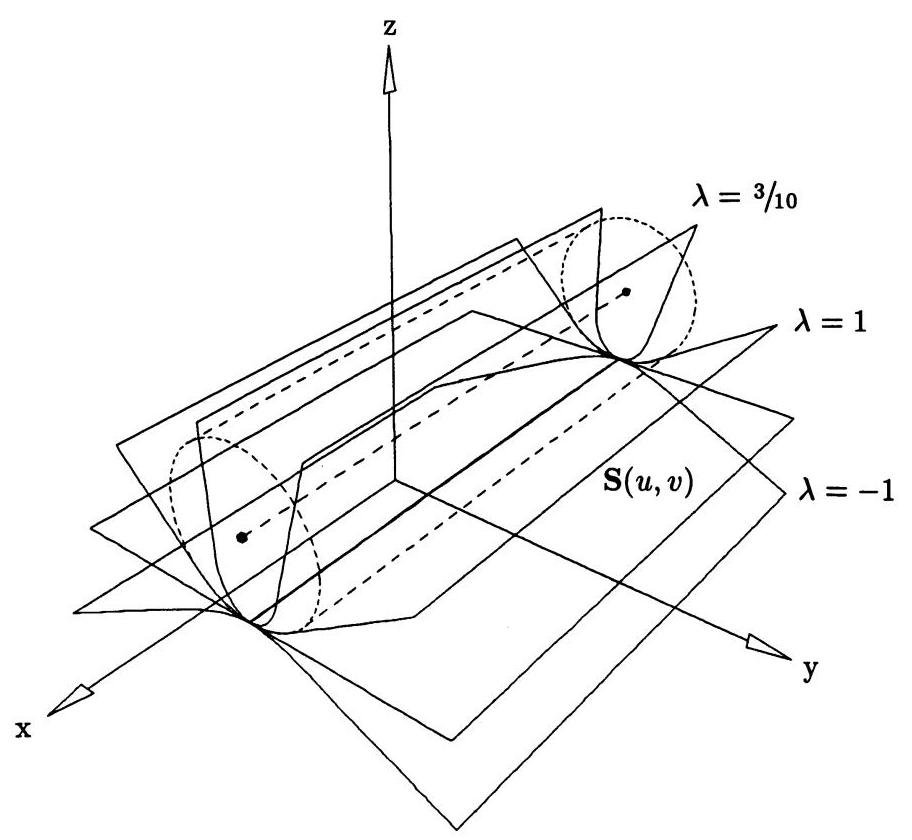
\includegraphics[max width=0.8\textwidth]{images/0193ba0d-ab19-7138-9798-cb281ce60de0_559_317_1236_912_840_0.jpg}
\end{center}
\hspace*{3em} 

图 11.34. 使用接触圆柱的表面弯曲示例， \(\lambda  = \left\{  {3/{}_{10},1, - 1}\right\}\) 。


\section{基于约束的曲线和表面造型}

接下来，我们提出了一种强制曲线或曲面在选定参数值处假定指定导数的方法。该方法允许任意阶数的导数，包括零阶导数，因此也包括点约束。通过约束一阶和二阶导数，可以控制曲线/曲面的切线和曲率。这些约束通过以最小化所有控制点的组合移动的方式重新定位控制点来满足。通过两步过程解决完全或欠定的线性方程组。这个两步解决方案允许基于约束的修改以交互速度实现。关于这个主题的更多材料可以在 [Fowl92, 93] 中找到。
\subsection{基于约束的曲线修改}
设 \(\;\mathbf{C}\left( u\right)  = \mathop{\sum }\limits_{{i = 0}}^{n}{R}_{i,p}\left( u\right) {\mathbf{P}}_{i}\;\) 为一条 NURBS 曲线。假设我们给定参数值 \(\left\{  {u}_{r}\right\}  ,r = 1,\ldots ,R\) 和一组导数约束， \(\left\{  {\Delta {\mathbf{D}}_{r}^{\left( k\right) }}\right\}  .\Delta {\mathbf{D}}_{r}^{\left( k\right) }\) 表示在 \(u = {u}_{r} \cdot  k\) 处 \(k\) 阶导数的变化可以取任何非负值，但通常为 \(k = 0,1,2\) ，因为这些值控制位置、切线和曲率的直观几何属性。注意，我们以导数变化的形式指定约束，而不是以目标值的形式。

现在固定 \(k\) 和 \(r\) ，并用 \({\mathbf{D}}_{r}^{\left( k\right) }\) 表示在 \(u = {u}_{r}\) 处 \(\mathbf{C}\left( u\right)\) 的 \(k\) 阶导数。然后

\[
{\mathbf{D}}_{r}^{\left( k\right) } = \mathop{\sum }\limits_{{i = 0}}^{n}{R}_{i,p}^{\left( k\right) }\left( {u}_{r}\right) {\mathbf{P}}_{i} \tag{11.65}
\]

其中 \({R}_{i,p}^{\left( k\right) }\) 表示基函数的 \(k\) 阶导数。如果曲线是非理性的，则使用算法 A2.3 计算基函数的导数。否则，使用在第 4.3 节中获得理性曲线导数所使用的相同技术计算 \({R}_{i,p}^{\left( k\right) }\) ，即

\[
{R}_{i,p}\left( u\right)  = \frac{w\left( u\right) {R}_{i,p}\left( u\right) }{w\left( u\right) } = \frac{{A}_{i}\left( u\right) }{w\left( u\right) }
\]

其中

\[
w\left( u\right)  = \mathop{\sum }\limits_{{j = 0}}^{n}{w}_{j}{N}_{j,p}\left( u\right)
\]

使用莱布尼茨法则对 \({A}_{i}\left( u\right)\) 进行微分得到

\[
{R}_{i,p}^{\left( k\right) }\left( u\right)  = \frac{{A}_{i}^{\left( k\right) }\left( u\right)  - \mathop{\sum }\limits_{{j = 1}}^{k}\left( \begin{array}{l} k \\  j \end{array}\right) {w}^{\left( j\right) }\left( u\right) {R}_{i,p}^{\left( k - j\right) }\left( u\right) }{w\left( u\right) } \tag{11.66}
\]

其中

\[
{A}_{i}^{\left( k\right) }\left( u\right)  = {w}_{i}{N}_{i,p}^{\left( k\right) }\left( u\right)
\]

在 \(u = {u}_{r}\) 处应用约束 \(\Delta {\mathbf{D}}_{r}^{\left( k\right) }\) ，我们得到新的 \(k\) 阶导数

\[
\mathop{\sum }\limits_{{i = 0}}^{n}{R}_{i,p}^{\left( k\right) }\left( {u}_{r}\right) \left( {{\mathbf{P}}_{i} + \Delta {\mathbf{P}}_{i}}\right)  = {\mathbf{D}}_{r}^{\left( k\right) } + \Delta {\mathbf{D}}_{r}^{\left( k\right) } \tag{11.67}
\]

因此

\[
\mathop{\sum }\limits_{{i = 0}}^{n}{R}_{i,p}^{\left( k\right) }\left( {u}_{r}\right) \Delta {\mathbf{P}}_{i} = \Delta {\mathbf{D}}_{r}^{\left( k\right) } \tag{11.68}
\]

方程 (11.68) 是关于 \(n + 1\) 个未知数 \(\left\{  {\Delta {\mathbf{P}}_{i}}\right\}\) 的一个线性方程(实际上是 \(p + 1\) 个未知数，因为 B 样条的局部支持性质)。我们注意到 \(\Delta {\mathbf{D}}_{r}^{\left( k\right) }\) 可以是零向量，实际上这就是指定某个点或导数不发生变化的方式。如果 \(M\) 是约束的总数， \(M \geq  R\) ，那么将方程 (11.68) 应用到每个约束上会产生一个关于 \(n + 1\) 个未知数的 \(M\) 个线性方程的系统，即

\[
B\left\lbrack  {\Delta {\mathbf{P}}_{i}}\right\rbrack   = \left\lbrack  {\Delta {\mathbf{D}}_{r}^{\left( k\right) }}\right\rbrack   \tag{11.69}
\]

在我们展示如何求解方程 (11.69) 之前，以下几点说明是重要的:

\begin{itemize}
\item 方程 (11.69) 假设约束有某种顺序；顺序可以是任意的，但一种自然的方法是先按 \(r\) 排序，然后按 \(k\) 排序。也就是说，假设 \(\Delta {\mathbf{D}}_{r}^{\left( k\right) }\) 的顺序为 \(\Delta {\mathbf{D}}_{1},\ldots ,\Delta {\mathbf{D}}_{M}\) ，并写成 \(\Delta {\mathbf{D}}_{i} = \Delta {\mathbf{D}}_{{r}_{i}}^{\left( {k}_{i}\right) }\) 那么 \(i < j\) 意味着 \({r}_{i} \leq  {r}_{j}\) ，并且，或者 \({r}_{i} < {r}_{j}\) 或 \({k}_{i} < {k}_{j}\) ;
\end{itemize}

\begin{itemize}
\item 由于 B 样条的局部支持性质以及约束通常仅在少数参数位置应用的事实，许多 \(B\) 的列可能为零；也就是说，未知数 \(\Delta {\mathbf{P}}_{i}\) 的数量少于 \(n + 1\) 。一个高效的算法应该建立方程 (11.69) 的系统，仅包含那些发生变化的 \(\Delta {\mathbf{P}}_{i}\) ; 用 \(N\) 表示实际的未知数 \(\Delta {\mathbf{P}}_{i}\) 的数量；
\end{itemize}

\begin{itemize}
\item 我们需要对方程 (11.69) 的精确解；然而，系统可能是欠定、完全确定或超定的，并且它可能没有精确解。对于后面提出的解法，我们需要一个欠定 \(\left( {M < N}\right)\) 或完全确定 \(\left( {M = N}\right)\) 的系统，其中 \(B\) 的所有行都是线性独立的。当指定的约束条件超过受影响控制点的度 \(p\) 或数量 \(N\) 时，就会出现超定系统 \(\left( {M > N}\right)\) 。显然，每个节点区间上不能指定超过 \(p + 1\) 的约束条件。如有必要，可以使用节点插入和/或度提升来确保一组约束产生一个欠定或完全确定的系统。如果 \(M \leq  N\) ，那么 \(B\) 的行的线性依赖通常不是问题 - 参见 [Scho66; Good81; Fowl93] 获取数学细节 - 但一个稳健的算法应该在解过程的第一步检查这一点；
\end{itemize}

\begin{itemize}
\item 通常设计者不需要指定施加约束的参数 \(\left\{  {u}_{r}\right\}\) ；理论上这些也可以是未知数，但这会导致非线性方程。因此，像往常一样，系统应该根据设计者选择的曲线点来选择参数。考虑到这些说明，我们现在将方程 (11.69) 写为
\end{itemize}

\[
B\left\lbrack  {\Delta {\mathbf{P}}_{{i}_{\ell }}}\right\rbrack   = \left\lbrack  {\Delta {\mathbf{D}}_{j}}\right\rbrack  \;\ell  = 1,\ldots ,N\;j = 1,\ldots ,M \tag{11.70}
\]

或者为了简洁

\[
{B\Delta }\mathbf{P} = \Delta \mathbf{D} \tag{11.71}
\]

目前，假设 \(M < N\) 。方程 (11.70) 存在无穷多解。我们希望找到最小长度解，即最小化所有控制点的组合移动的解(最小化 \(N\) 维向量 \(\Delta \mathbf{P}\) 的长度)。根据线性代数，我们可以将 \(N\) 向量 \(\Delta \mathbf{P}\) 表示为两个相互正交的分量，一个在 \(B\) 的行空间中，另一个在 \(B\) 的零空间中，即

\[
\Delta \mathbf{P} = {B}^{T}\lambda  + \mathbf{z} \tag{11.72}
\]

其中 \(\lambda\) 是某个 \(M\) 向量 \(B\mathbf{z} = 0\) 和 \(\left( {{\lambda }^{T}B}\right)  \cdot  \mathbf{z} = 0\) 。因此可以得出

\[
{\left| \Delta \mathbf{P}\right| }^{2} = {\left( {B}^{T}\lambda  + \mathbf{z}\right) }^{T} \cdot  \left( {{B}^{T}\lambda  + \mathbf{z}}\right)
\]

\[
= {\left( {B}^{T}\lambda \right) }^{T} \cdot  \left( {{B}^{T}\lambda }\right)  + {\mathbf{z}}^{T} \cdot  \mathbf{z}
\]

\[
= {\left| {B}^{T}\lambda \right| }^{2} + {\left| \mathbf{z}\right| }^{2} \tag{11.73}
\]

从方程 (11.71) 和 (11.72) 中我们得到

\[
\Delta \mathbf{D} = {B\Delta }\mathbf{P}
\]

\[
= B\left( {{B}^{T}\lambda  + \mathbf{z}}\right)
\]

\[
= B{B}^{T}\lambda  + B\mathbf{z}
\]

\[
= B{B}^{T}\lambda  \tag{11.74}
\]

因此

\[
\lambda  = {\left( B{B}^{T}\right) }^{-1}\Delta \mathbf{D} \tag{11.75}
\]

由于 \(\mathbf{z}\) 的分量与系统无关，但它们对 \(\Delta \mathbf{P}\) 的长度有贡献(根据方程 [11.73])，我们通过设定 \(\mathbf{z} = 0\) 来获得方程 (11.70) 的最小长度解。将方程 (11.75) 代入 (11.72) 得到

\[
\Delta \mathbf{P} = {A\Delta }\mathbf{D}\;\text{ where }A = {B}^{T}{\left( B{B}^{T}\right) }^{-1} \tag{11.76}
\]

如果 \(B{B}^{T}\) 的行 \(B\) 线性无关，则矩阵 \(B{B}^{T}\) 是非奇异的。最后，如果 \(M = N\) ，则方程 (11.70) 有唯一解

\[
\Delta \mathbf{P} = {A\Delta }\mathbf{D}\;\text{ where }A = {B}^{-1} \tag{11.77}
\]

我们指出，也可以(并且非常有用)限制某些控制点不发生变化。这在数学上简单地通过将 \(B\) 的相应列设置为零来实现。在算法上，这意味着相应的 \(\Delta {\mathbf{P}}_{{i}_{\ell }}\) 不出现在方程 (11.70) 中，并且 \(N\) 减少了 1。通常，一个约束影响 \(p + 1\) 个控制点，并且在任何跨度中可以指定最多 \(p + 1\) 个约束。如果一个控制点被限制不移动，那么这将减少 \(p\) 在任何受此控制点影响的跨度中可以指定的约束数量。我们在下面给出这些例子的说明。

方程 (11.76)(或方程 [11.77])表示解决过程中的第一步。在进行第二步之前，我们总结了将我们带到这一点的事件序列:

1. 设计师在曲线上选择点，产生由系统确定的参数 \(\left\{  {u}_{r}\right\}\) ，在这些参数上施加约束；他同时指明在每个参数上施加何种类型的约束，但在此阶段不需要实际指定约束；

2. 系统建立方程 (11.70)；如果它是超定的，系统要么通知设计师以便他可以修改选择，要么通过节点插入和/或提升次数的方式添加控制点，使得结果方程组是欠定或完全确定的；

3. 然后通过方程 (11.76) 或 (11.77) 计算矩阵 \(A\) 。

设计师现在可以交互式地指定约束 \(\left\lbrack  {\Delta {\mathbf{D}}_{j}}\right\rbrack\) 。每次约束发生变化时，矩阵 \(A\) 必须与新的向量 \(\left\lbrack  {\Delta {\mathbf{D}}_{j}}\right\rbrack\) 相乘，以产生控制点位置的变化 \(\left\lbrack  {\Delta {\mathbf{P}}_{{i}_{\ell }}}\right\rbrack\) 。相关的控制点随后被更新为

\[
{\widehat{\mathbf{P}}}_{{i}_{\ell }} = {\mathbf{P}}_{{i}_{\ell }} + \Delta {\mathbf{P}}_{{i}_{\ell }}\;\ell  = 1,\ldots ,N \tag{11.78}
\]

\section*{示例}

Ex11.1 图 11.35a 显示了由 \({\mathbf{P}}_{0},\ldots ,{\mathbf{P}}_{7}\) 定义的立方曲线，以及 \(U =\)  \(\{ 0,0,0,0,1/5,2/5,3/5,4/5,1,1,1,1\}\) 。我们在 \(u = 1/2\) 应用一个点约束

\[
\Delta {\mathbf{D}}_{1} = \Delta {\mathbf{D}}_{1}^{\left( 0\right) } = \left( {{0.04}, - {0.08},0}\right)
\]

然后

\[
{B\Delta }\mathbf{P} = \left\lbrack  {\Delta {\mathbf{D}}_{1}}\right\rbrack
\]

其中 \(B\) 是 \(1 \times  4\) 矩阵

\[
B = \left\lbrack  {{R}_{2,3}\left( \frac{1}{2}\right) ,{R}_{3,3}\left( \frac{1}{2}\right) ,{R}_{4,3}\left( \frac{1}{2}\right) ,{R}_{5,3}\left( \frac{1}{2}\right) }\right\rbrack
\]

而 \(\Delta \mathbf{P}\) 是具有以下分量的 \(4 \times  1\) 列向量

\[
\Delta {\mathbf{P}}_{2},\Delta {\mathbf{P}}_{3},\Delta {\mathbf{P}}_{4},\Delta {\mathbf{P}}_{5}
\]

因此， \(B{B}^{T}\) 是一个 \(1 \times  1\) 矩阵，而 \(A = {B}^{T}{\left( B{B}^{T}\right) }^{-1}\) 是一个 \(4 \times  1\) 矩阵

\begin{center}
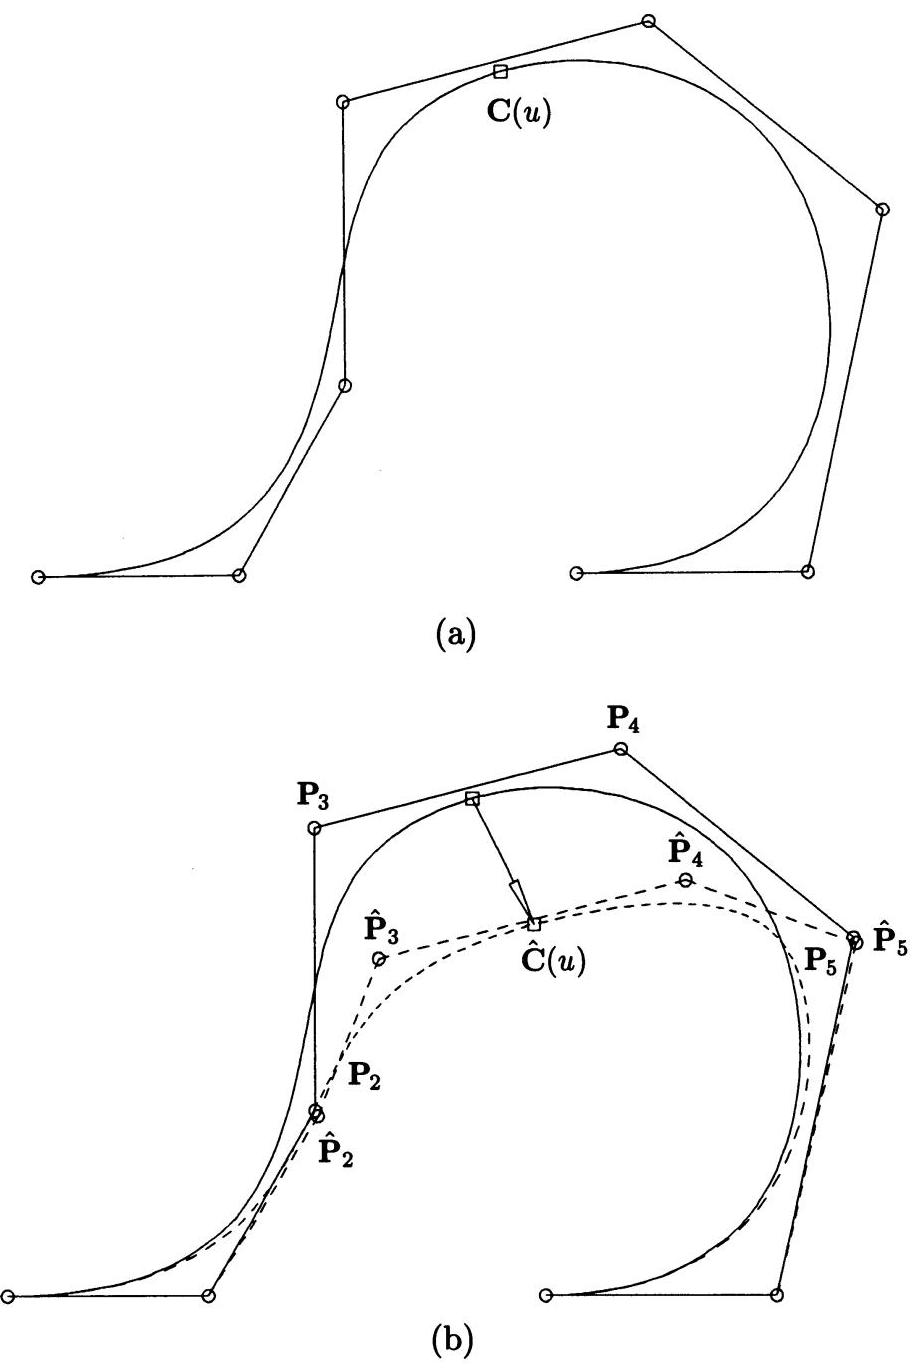
\includegraphics[max width=0.8\textwidth]{images/0193ba0d-ab19-7138-9798-cb281ce60de0_564_314_252_917_1369_0.jpg}
\end{center}
\hspace*{3em} 

图 11.35. 基于约束的曲线修改使用位置约束。 (a) 原始立方曲线及要移动的点；(b) 所有四个局部控制点均可移动；(c) 仅允许 \({\mathbf{P}}_{3}\) 和 \({\mathbf{P}}_{4}\) 移动；(d) 仅允许 \({\mathbf{P}}_{3}\) 移动。

具有以下分量

\[
{a}_{0},{a}_{1},{a}_{2},{a}_{3}
\]

因此

\[
\Delta {\mathbf{P}}_{i} = {a}_{i - 2}\Delta {\mathbf{D}}_{1}\;i = 2,3,4,5
\]

应用 \(\Delta {\mathbf{P}}_{i}\) 的结果如图 11.35b 所示。注意到 \({\mathbf{P}}_{3}\) 和 \({\mathbf{P}}_{4}\) 移动得最多，因为这些控制点具有最大的

560 形状修改工具

图 11.35. (续)

\begin{center}
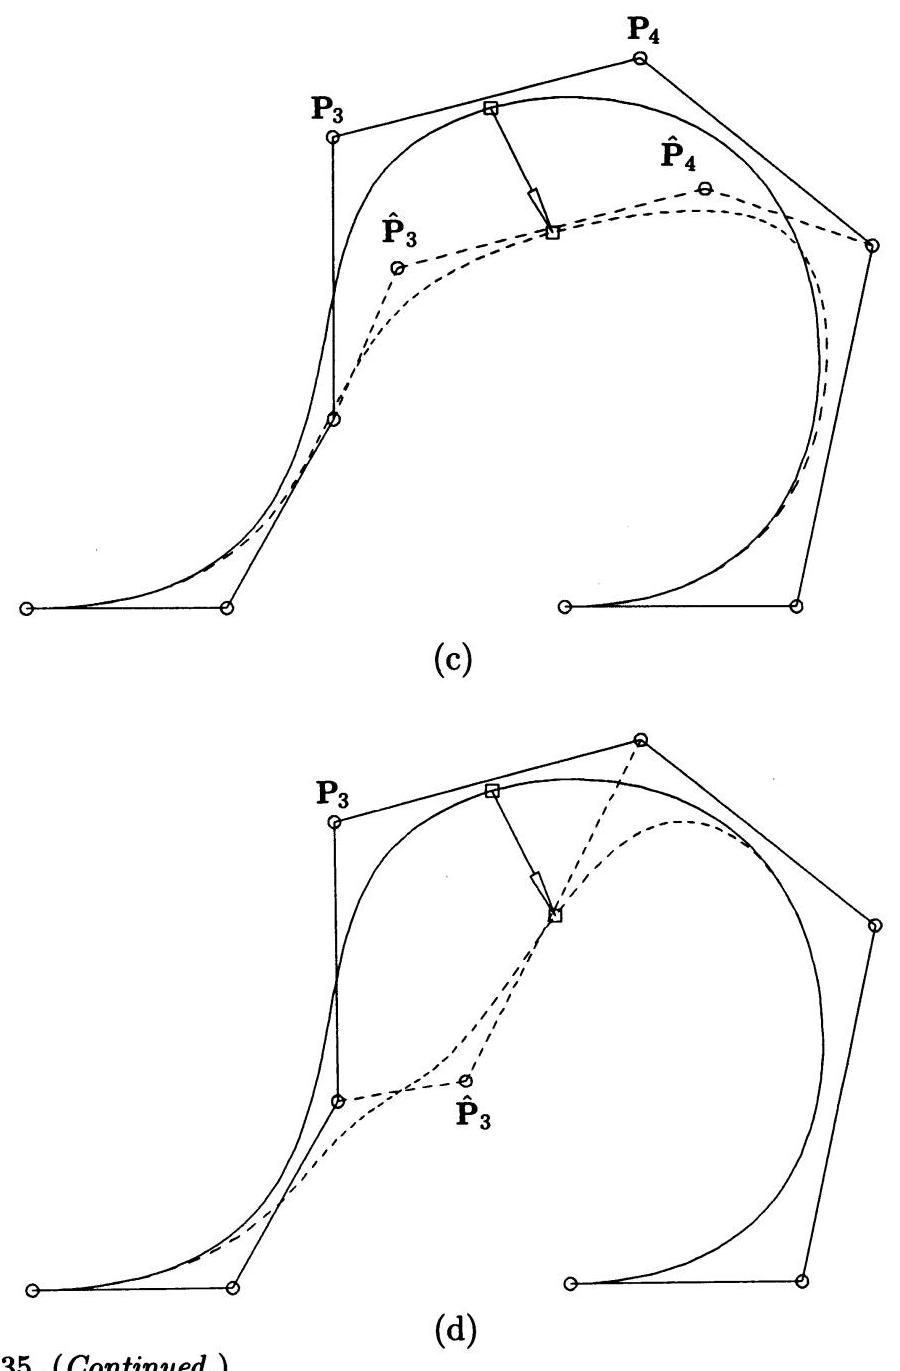
\includegraphics[max width=0.8\textwidth]{images/0193ba0d-ab19-7138-9798-cb281ce60de0_565_315_246_900_1371_0.jpg}
\end{center}
\hspace*{3em} 

在 \(u = 1/2\) 处对曲线的影响。我们可以限制 \({\mathbf{P}}_{2}\) 和 \({\mathbf{P}}_{5}\) 的移动。然后 \(B\) 是 \(1 \times  2\) 矩阵

\[
B = \left\lbrack  {{R}_{3,3}\left( \frac{1}{2}\right) ,{R}_{4,3}\left( \frac{1}{2}\right) }\right\rbrack
\]

并且 \(\Delta \mathbf{P}\) 的分量是 \(\Delta {\mathbf{P}}_{3}\) ，而 \(\Delta {\mathbf{P}}_{4}.A\) 的分量是 \({a}_{0}\) 和 \({a}_{1}\) (与上面的 \({a}_{0},{a}_{1}\) 不同)，并且

\[
\Delta {\mathbf{P}}_{i} = {a}_{i - 3}\Delta {\mathbf{D}}_{1}\;i = 3,4
\]

图 11.35c 显示了仅允许 \({\mathbf{P}}_{3}\) 和 \({\mathbf{P}}_{4}\) 变化的结果，而图 11.35d 则说明了仅允许 \({\mathbf{P}}_{3}\) 移动的情况。

这个例子清楚地表明，对于给定的一组点和导数约束，通常在指定多少个以及哪些控制点应该变化时存在灵活性，而这个选择会影响相应曲线变化的范围和外观(例如，对称性)。然而，对于设计师而言，处理控制点可能不如对曲线施加纯点和导数约束直观。一个良好的用户界面应该同时提供一组合理的默认值和方便的工具，以便更复杂的设计师限制控制点的移动。最后，请注意，任何控制点的限制必须纳入方程 (11.70) 和解决过程的第一阶段。

在图11.36a-11.36c中，展示了点和导数约束。图11.36a仅显示了导数约束的应用，同时允许 \({\mathbf{P}}_{3},{\mathbf{P}}_{4}\) 和 \({\mathbf{P}}_{5}\) 移动。在 \(u = {0.556}\) 处，第一导数向量的大小增加，导致局部张力效应。如果仅允许一个控制点移动，如图11.36b所示，观察结果非常有趣。曲线采用了新的导数，但由于缺乏位置约束，它遭受了位置位移。在图11.36c中，通过约束曲线在 \(u = {0.556}\) 处不移动，并假设通过减小旧导数的大小获得的新导数，解决了这个问题。允许两个控制点移动，以获得一个不被过度确定的方程组。

最后，我们提到Fowler和Bartels [Fowl93] 提供了一种不同(但等效)的方法来表示方程(11.76)和(11.77)中的矩阵 \(A\) 。这种方法在数学上稍微复杂一些，但在某些情况下更有效。

\begin{center}
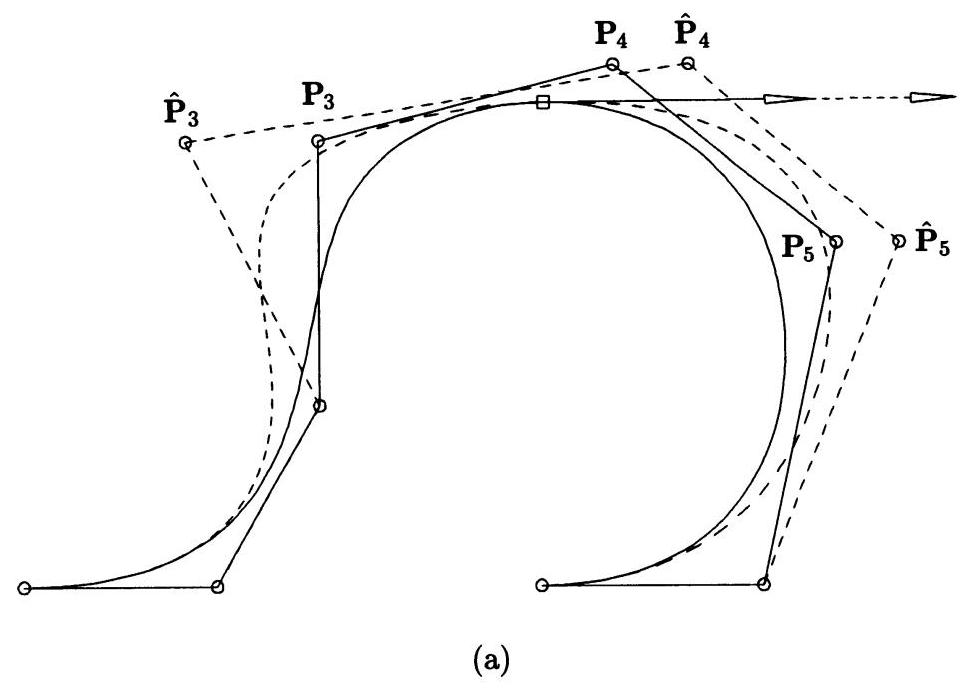
\includegraphics[max width=0.8\textwidth]{images/0193ba0d-ab19-7138-9798-cb281ce60de0_566_281_1301_966_689_0.jpg}
\end{center}
\hspace*{3em} 

图11.36. 基于约束的曲线修改，使用位置和导数约束。(a) 应用导数约束，并允许 \({\mathbf{P}}_{3},{\mathbf{P}}_{4}\) 和 \({\mathbf{P}}_{5}\) 移动；(b) 应用导数约束，仅允许 \({\mathbf{P}}_{4}\) 移动；(c) 应用导数和位置约束，并允许 \({\mathbf{P}}_{3}\) 和 \({\mathbf{P}}_{4}\) 移动。

562 形状修改工具

\begin{center}
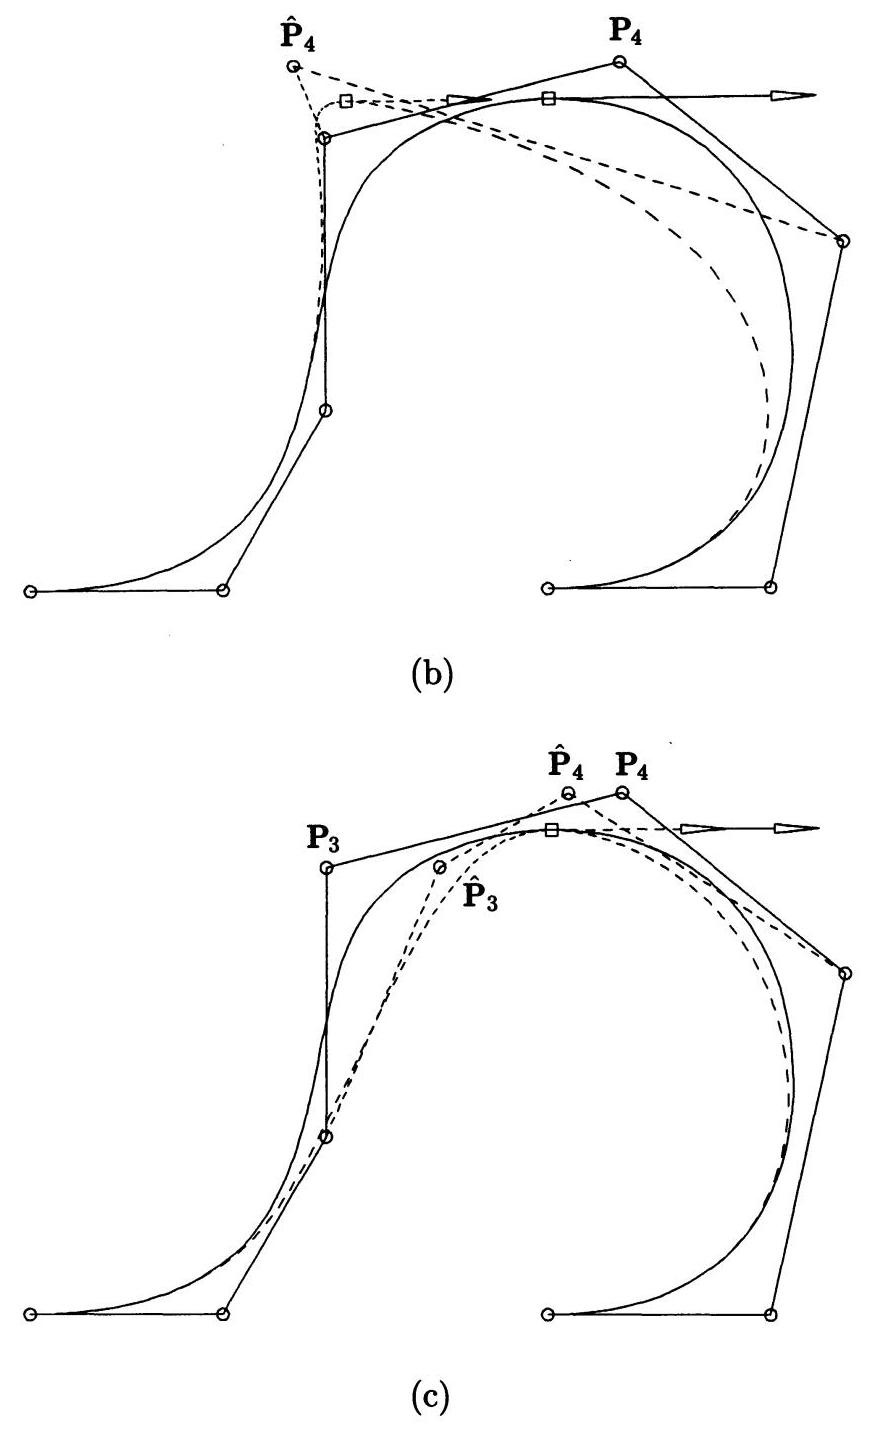
\includegraphics[max width=0.7\textwidth]{images/0193ba0d-ab19-7138-9798-cb281ce60de0_567_340_242_870_1431_0.jpg}
\end{center}
\hspace*{3em} 

图11.36. (续)



\subsection{基于约束的表面修改}

设 \(\;\mathbf{S}\left( {u,v}\right)  = \mathop{\sum }\limits_{{i = 0}}^{n}\mathop{\sum }\limits_{{j = 0}}^{m}{R}_{i,p;j,q}\left( {u,v}\right) {\mathbf{P}}_{i,j}\;\) 为一个 \(\;\left( {p,q}\right)\) 次NURBS曲面。在本节中，我们选择将 \(\mathbf{S}\left( {u,v}\right)\) 写成以下形式

\[
\mathbf{S}\left( {u,v}\right)  = \mathop{\sum }\limits_{{s = 0}}^{{\left( {n + 1}\right) \left( {m + 1}\right)  - 1}}{R}_{s}\left( {u,v}\right) {\mathbf{P}}_{s} \tag{11.79}
\]

其中

\[
s = j\left( {n + 1}\right)  + i \tag{11.80}
\]

我们称 \(s\) 为对应于 (i, j) 的绝对地址。注意到

\[
{\mathbf{P}}_{s} = {\mathbf{P}}_{i,j}\;{R}_{s}\left( {u,v}\right)  = {R}_{i,p;j,q}\left( {u,v}\right)  \tag{11.81}
\]

其中

\[
i = s{\;\operatorname{mod}\;n} + 1\;j = \frac{s}{n + 1} \tag{11.82}
\]

如果 \(\mathbf{S}\left( {u,v}\right)\) 是非有理的，则 \({R}_{s}\left( {u,v}\right)  = {N}_{i,p}\left( u\right) {N}_{j,q}\left( v\right)\) ，其中 \(i\) 和 \(j\) 由公式 (11.82) 定义。现在假设我们给定了一组点和偏导数约束 \(\left\{  {\Delta {\mathbf{D}}_{r}^{\left( k,\ell \right) }}\right\}  ,k,\ell  \geq  0\) ，这些约束在参数位置 \(\left\{  {\left( u,v\right) }_{r}\right\}  ,r = 1,\ldots ,R\) 处指定。那么对于每个 \(r\) 我们有

\[
\mathop{\sum }\limits_{{s = 0}}^{{+1)\left( {m + 1}\right)  - 1}}{R}_{s}^{\left( k,\ell \right) }\left( {\left( u,v\right) }_{r}\right) \Delta {\mathbf{P}}_{s} = \Delta {\mathbf{D}}_{r}^{\left( k,\ell \right) } \tag{11.83}
\]

偏导数 \({R}_{s}^{\left( k,\ell \right) }\left( {\left( u,v\right) }_{r}\right)\) 可以以与第 4.5 节中描述的 \({\mathbf{S}}^{\left( k,\ell \right) }\left( {u,v}\right)\) 完全相同的方式计算。然后，正如曲线的情况一样，我们可以建立 \(M \times  N\) 线性方程组

\[
B\left\lbrack  {\Delta {\mathbf{P}}_{{s}_{\alpha }}}\right\rbrack   = \left\lbrack  {\Delta {\mathbf{D}}_{r}^{\left( k,\ell \right) }}\right\rbrack  \;\alpha  = 1,\ldots ,N \tag{11.84}
\]

\(M\) 是约束的数量 \(\left( {M \geq  R}\right)\) ，而 \(N\) 是可以自由移动的控制点的数量。一般来说，一个约束涉及 \(\left( {p + 1}\right)  \times  \left( {q + 1}\right)\) 个控制点，但一个控制点可以通过不将其包含在公式 (11.84) 中而保持固定。方程 (11.84) 可以是欠定的、完全确定的或超定的。如果是超定的，则可以使用节点插入和/或次数提升来获得欠定或完全确定的系统。

方程 (11.84) 的求解方式与曲线的情况完全相同，即

\[
\left\lbrack  {\Delta {\mathbf{P}}_{{s}_{\alpha }}}\right\rbrack   = A\left\lbrack  {\Delta {\mathbf{D}}_{r}^{\left( k,\ell \right) }}\right\rbrack   \tag{11.85}
\]

其中

\[
A = {B}^{T}{\left( B{B}^{T}\right) }^{-1} \tag{11.86}
\]

(或 \(A = {B}^{-1}\) 如果方程 [11.84] 是完全确定的)。这产生了控制点的最小组合移动。最后一步是

\[
{\widehat{\mathbf{P}}}_{{s}_{\alpha }} = {\mathbf{P}}_{{s}_{\alpha }} + \Delta {\mathbf{P}}_{{s}_{\alpha }}\;\alpha  = 1,\ldots ,N \tag{11.87}
\]

尽管基于曲线和曲面的约束修改的数学几乎是相同的，但设置矩阵 \(A\) 所需的软件对于曲面来说更为复杂。算法 A11.1 说明了一种可能的解决方案。除了定义曲面的数据外，还输入一个结构列表 (CList)。该列表包含 \(R\) 个节点；每个节点包含一对参数 \({\left( u,v\right) }_{r}\) 和在该点应用的约束类型列表(实际约束不被输入)。输出包括:

M : 约束的数量(以及 \(\mathbf{A}\) 的列数)；

N : 变化的控制点数量(以及 \(\mathbf{A}\) 的行数)；

A[] [] : 矩阵 \(A\) ；

CpInd[] : 变化的控制点的绝对地址 \({s}_{\alpha }\) 。

此外，返回以下整数值之一:

0 : 无错误；

1 : 系统是过定的；

2 : 矩阵是奇异的( \(B\) 的行不是线性独立的)。

为了构建 A 和 CpInd，使用了三个局部二维数组 B[M][Nmax]、FreeCp[p+1][q+1] 和 Map[n+1][m+1]，以及一个四维数组 Funs 和两个新例程 FreeCtrlPts(u, v, FreeCp) 和 RatDersBasisFuns(u, v, Funs)。B 包含方程 (11.84) 的矩阵 \(B\) 。如果 \({\mathbf{P}}_{i,j}\) 不是由方程 (11.84) 定义的系统的一部分，则 Map[i] \(\left\lbrack  j\right\rbrack   =  - 1\) ；否则，Map[i] \(\left\lbrack  j\right\rbrack   = \alpha  \geq  0\) 是 CpInd 的索引，而 CpInd \(\left\lbrack  \alpha \right\rbrack   = s\) 是对应于 (i, j) 的绝对地址。对于给定的 (u, v)，FreeCtrlPts(   ) 返回布尔数组 FreeCp，指示在 (u, v) 处影响表面的可能 \(\left( {p + 1}\right)  \times  \left( {q + 1}\right)\) 控制点中哪些是可以移动的。这个例程可以以多种有意义的方式实现，因此我们在这里不再详细说明。例程 RatDersBasisFuns(u, v, Funs) 返回基函数及其偏导数。Funs \(\left\lbrack  k\right\rbrack  \left\lbrack  1\right\rbrack  \left\lbrack  i\right\rbrack  \left\lbrack  j\right\rbrack\) 是 (i, j)th 基函数的 \(\left( {k,\ell }\right)\) 次偏导数。

\HRule

\section*{ALGORITHM A11.1}

ConstBasedSurfMod1(n, m, p, q, U, V, Pw, CList, R, M, N, A, CpInd)

\hspace*{3em} \{ /* Build the A matrix for surface constraints */

\hspace*{6em} /* Input: n, m, p, q, U, V, Pw, CList, R */

\hspace*{6em} /* Output: M, N, A, CpInd */

\hspace*{2em} Loop through the list CList and count constraints

\hspace*{5em} to obtain M.

\hspace*{2em} Nmax \(=\) Max \(\left( {\left( {n + 1}\right)  * \left( {m + 1}\right) ,R * \left( {p + 1}\right)  * \left( {q + 1}\right) }\right) ;/ *\) Max possible \(N * /\)

\hspace*{2em} for (i=0; i<M; i++)

\hspace*{5em} for \(\left( {j = 0;j < \text{ Nmax; }j +  + }\right) \;B\left\lbrack  i\right\rbrack  \left\lbrack  j\right\rbrack   = {0.0}\) ;

\hspace*{2em} for (i = 0; i<=n; i++)

\hspace*{5em} for \(\left( {j = 0;j <  = m;j +  + }\right) \;\operatorname{Map}\left\lbrack  i\right\rbrack  \left\lbrack  j\right\rbrack   =  - 1\) ;

\hspace*{2em} brow \(= 0;\;N = 0;\;/ * N\) is computed in this loop \(* /\)

\hspace*{2em} for (r=1; r<=R; r++)

\hspace*{5em} \{

\hspace*{5em} Extract (u, v) value from the \(r\) th list node.

\hspace*{5em} FreeCtrlPts(u, v, FreeCp);

\hspace*{5em} uspan = FindSpan(n, p, u, U);

\hspace*{5em} vspan = FindSpan(m, q, v, V);

\hspace*{5em} for (i = 0; i<=p; i++)

\hspace*{5em} for (j=0; j<=q; j++)

\hspace*{7em} if (FreeCp[i][j])

\hspace*{9em} \{ /* This ctrl pt is free to move */

\hspace*{9em} iup = i+uspan-p; jvq = j+vspan-q;

\hspace*{9em} if (Map[iup][jvq] == -1)

\hspace*{12em} \{ /* Ctrl pt not yet in Eq. system */

\hspace*{12em} Map[iup][jvq] = N;

\hspace*{12em} \(\operatorname{CpInd}\left\lbrack  \mathrm{N}\right\rbrack   = {jvq} * \left( {\mathrm{n} + 1}\right)  + {iup};\)

\hspace*{12em} \(\mathrm{N} = \mathrm{N} + 1\) ;

\hspace*{11em} \}

\hspace*{9em} \}

\hspace*{3em} /* Compute required functions */

\hspace*{3em} RatDersBasisFuns(u, v, Funs);

\hspace*{3em} Loop through each type of constraint for this(u, v)and \({do}\) :

\hspace*{5em} \{

\hspace*{5em} Set \(k\) and \(\ell\) indicating which derivative.

\hspace*{5em} for (i = 0; i<=p; i++)

\hspace*{7em} for (j=0; j<=q; j++)

\hspace*{9em} \{

\hspace*{9em} alf = Map[i+uspan-p][j+vspan-q];

\hspace*{9em} if (alf >= 0) B[brow][alf] = Funs[k][l][i][j];

\hspace*{9em} \}

\hspace*{5em} brow = brow+1;

\hspace*{5em} \} /* End of loop through each type of constraint */

\hspace*{1em} \} /* End of for-loop: \(r = 1,\ldots ,R * /\)

if \(\left( {M > N}\right)\) return (1); /* system overdetermined */

if (M == N)

\hspace*{3em} if(B singular)return(2);

\hspace*{5em} else

\hspace*{5em} \{

\hspace*{5em} \(A = {B}^{-1};\;\) return \(\left( 0\right) ;\)

\hspace*{5em} \}

if \(\left( {B{B}^{T}}\right.\) singular) return(2);

\hspace*{3em} else

\hspace*{3em} \{

\hspace*{3em} \(\mathbf{A} = {B}^{T}{\left( B{B}^{T}\right) }^{-1};\;\operatorname{return}\left( 0\right) ;\)

\hspace*{2em} \}

\}

\HRule

图 11.37-11.39 显示了应用表面约束的示例。在图 11.37a 和 \({11.37}\mathrm{\;b}\) 中，在 \(u = v = 1/2\) 处施加了一个点约束，允许所有影响该点表面的控制点移动。图 11.37a 显示了新的控制网，图 11.37b 则说明了表面形状的变化。请注意，局部域周围的控制点移动非常有限。图 11.38a 和 \({11.38}\mathrm{\;b}\) 显示了如果仅允许 \({\mathbf{P}}_{1,2},{\mathbf{P}}_{2,2}\) 和 \({\mathbf{P}}_{4,2}\) 在形状中移动会发生什么。最后，在图 11.39a 和 \({11.39}\mathrm{\;b}\) 中施加了偏导数和位置约束。在图 11.39a 中，偏导数的大小增加，导致了张力效应，而在图 11.39b 中，偏导数围绕点 \(\mathbf{S}\left( {1/2,1/2}\right)\) 旋转，导致表面形状扭曲。

\begin{center}
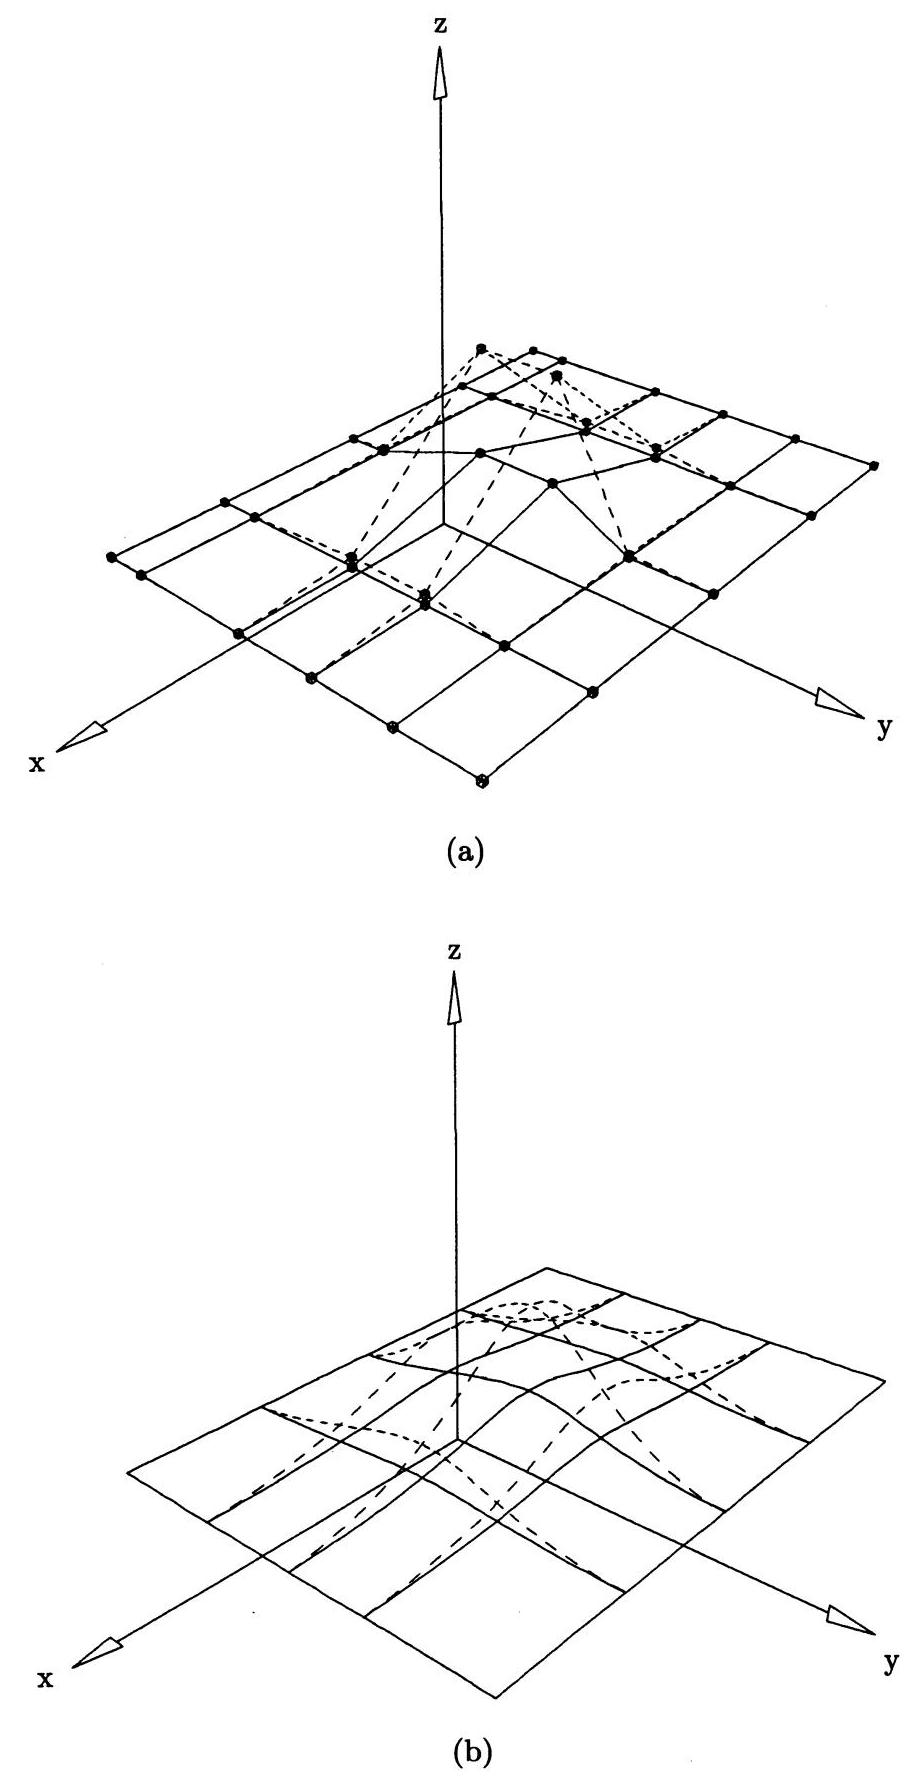
\includegraphics[max width=0.8\textwidth]{images/0193ba0d-ab19-7138-9798-cb281ce60de0_571_308_253_916_1779_0.jpg}
\end{center}
\hspace*{3em} 

图 11.37. 基于约束的表面修改，带有位置约束。(a) 显示所有移动的局部控制点的表面网；(b) 形状发生变化的表面。

\begin{center}
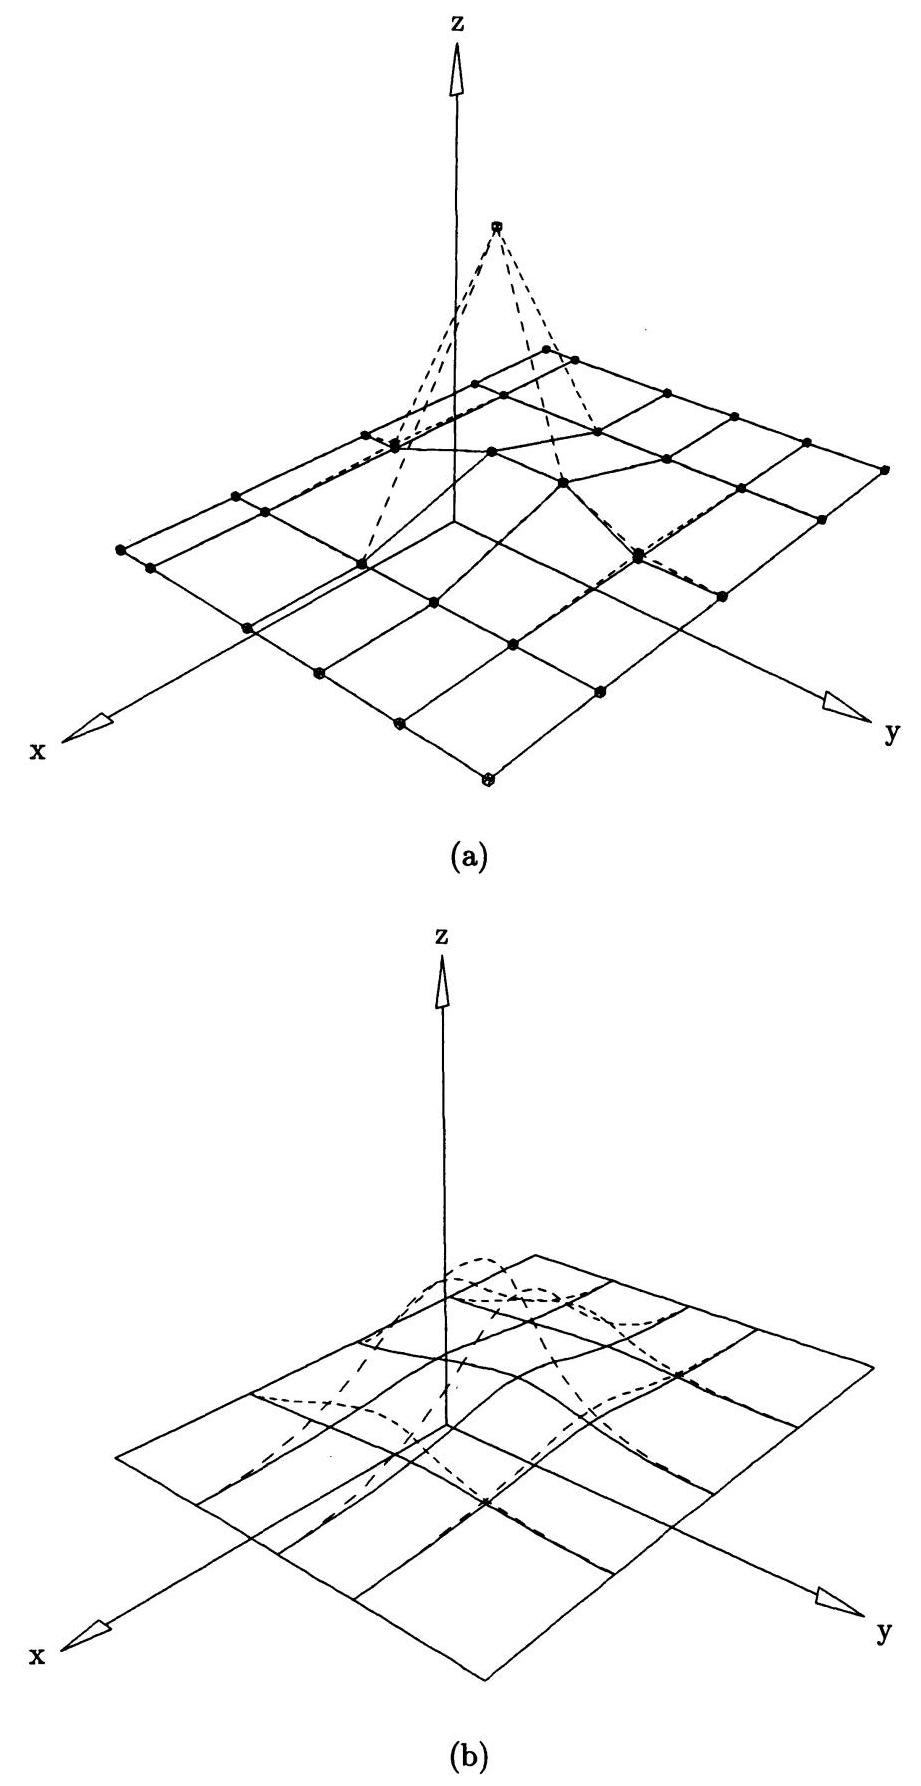
\includegraphics[max width=0.8\textwidth]{images/0193ba0d-ab19-7138-9798-cb281ce60de0_572_306_250_921_1786_0.jpg}
\end{center}
\hspace*{3em} 

图 11.38. 基于约束的表面修改，带有位置约束。(a) 显示仅允许 \({\mathbf{P}}_{1,2},{\mathbf{P}}_{2,2}\) 和 \({\mathbf{P}}_{4,2}\) 移动的表面网；(b) 形状发生变化的表面。

\begin{center}
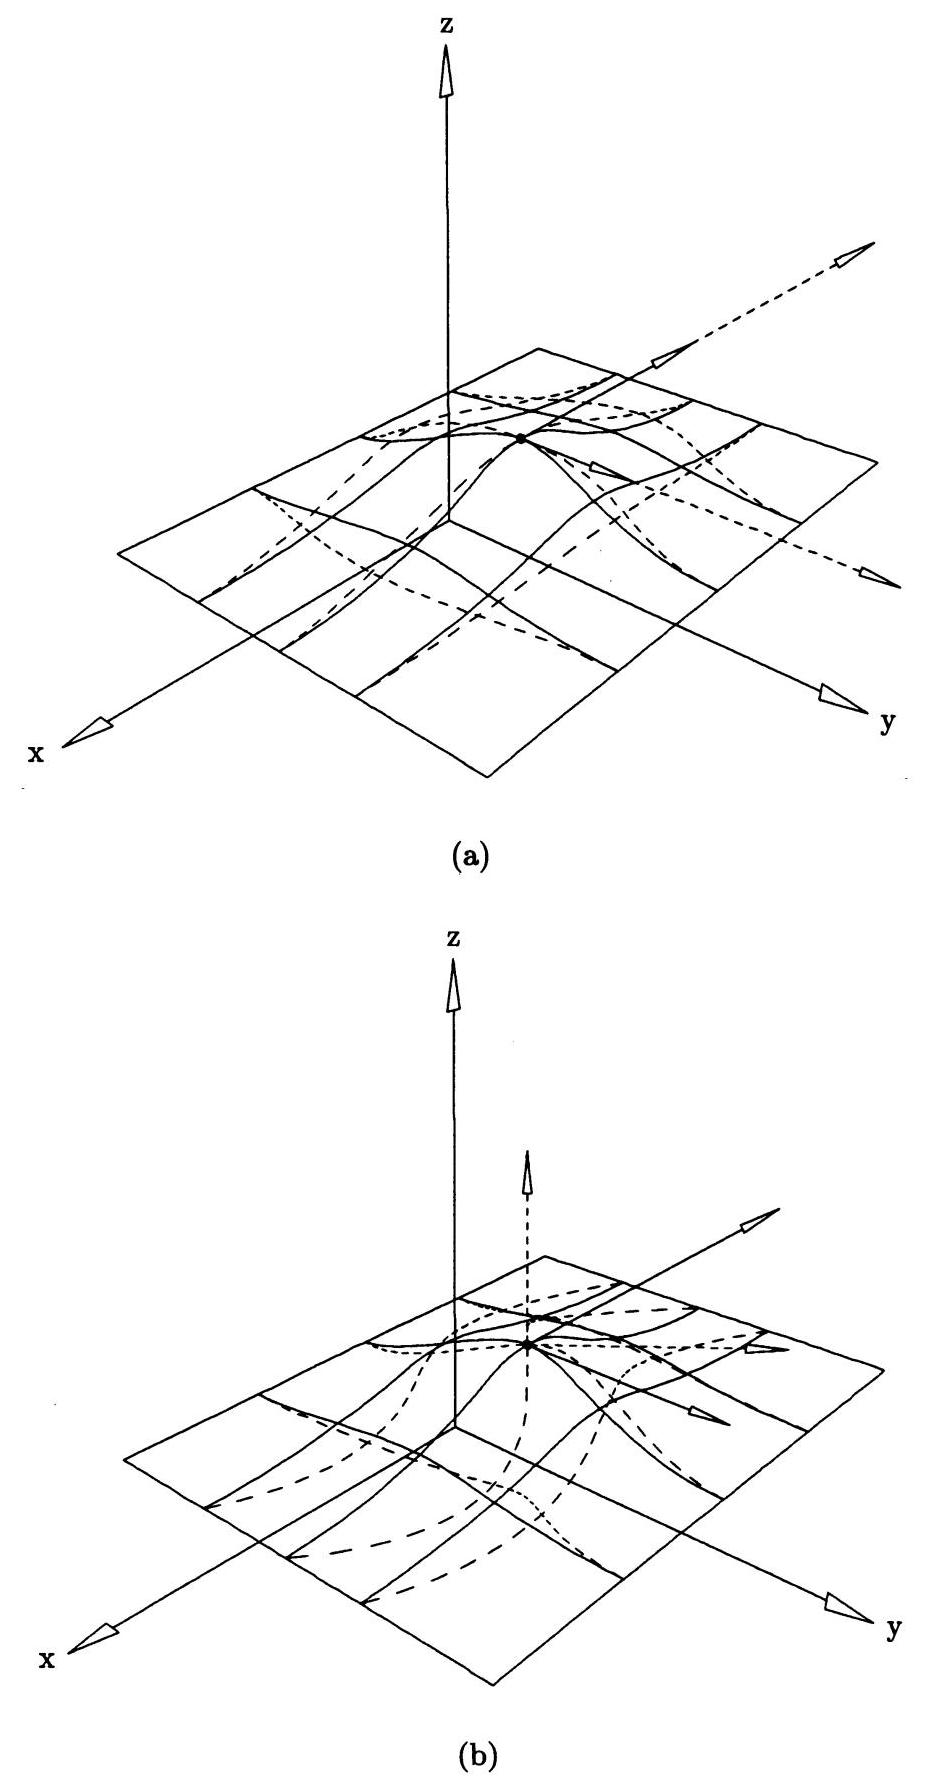
\includegraphics[max width=0.8\textwidth]{images/0193ba0d-ab19-7138-9798-cb281ce60de0_573_302_249_925_1783_0.jpg}
\end{center}
\hspace*{3em} 

图 11.39. 基于约束的表面修改，带有位置和导数约束。(a) 偏导数大小的增加引发局部张力效应；(b) 偏导数方向的变化引发局部扭曲效应。

最后，我们指出，Fowler [Fowl92] 提出了一个替代(等效)解决方案，用于求解 \(\Delta {\mathbf{P}}_{i,j}\) ，该方案利用了 \(\mathbf{S}\left( {u,v}\right)\) 的张量积结构。它的通用性不如这种方法，但在某些情况下更为高效。


\clearpage
    

\end{document}


